\documentclass[11pt,a4paper]{article}

% ==============================================================================
% PACKAGES & ZERO-OVERFLOW PAGE GEOMETRY
% ==============================================================================
\usepackage[utf8]{inputenc}
\usepackage[T1]{fontenc}
\usepackage{lmodern}
\usepackage[margin=2.1cm, headheight=14pt]{geometry}
\usepackage{amsmath,amssymb,amsfonts,amsthm,mathtools}
\usepackage{bm}
\usepackage{booktabs}
\usepackage{array}
\usepackage{multirow}
\usepackage{graphicx}
\usepackage{xcolor}
\usepackage{float}
\usepackage{enumitem}
\usepackage{tikz}
\usepackage{pgfplots}
\pgfplotsset{compat=1.18}
\usepackage[colorlinks=true,linkcolor=blue!70!black,citecolor=teal!70!black,urlcolor=blue!80!black,pdfencoding=auto,psdextra]{hyperref}

\setlength{\emergencystretch}{3em}
\allowdisplaybreaks

% ==============================================================================
% EPISTEMOLOGICAL CLASSIFICATION BADGES (RULE R1)
% ==============================================================================
\newcommand{\catD}{\textbf{\textcolor{blue!75!black}{[D]}}}
\newcommand{\catH}{\textbf{\textcolor{orange!85!black}{[H]}}}
\newcommand{\catN}{\textbf{\textcolor{teal!75!black}{[N]}}}

% ==============================================================================
% THEOREM ENVIRONMENTS
% ==============================================================================
\newtheorem{theorem}{Theorem}[section]
\newtheorem{lemma}[theorem]{Lemma}
\newtheorem{proposition}[theorem]{Proposition}
\newtheorem{corollary}[theorem]{Corollary}
\theoremstyle{definition}
\newtheorem{definition}[theorem]{Definition}
\newtheorem{postulate}[theorem]{Postulate}
\newtheorem{hypothesis}[theorem]{Hypothesis}
\newtheorem{observation}[theorem]{Numerical Observation}
\theoremstyle{remark}
\newtheorem{remark}[theorem]{Remark}

% ==============================================================================
% TITLE, AUTHOR, AFFILIATION & ABSTRACT
% ==============================================================================
\title{\vspace{-1.3cm}\textbf{\Large Covariant Bitemporal Geometrodynamics (CBG): Variational Principles, 5D Laplacian Field Equations, and the Informational Resolution of Cosmological and Quantum Singularities}\\[0.18cm]
\large The 5D Bitemporal Manifold $\mathcal{M}_{3,2} = (\mathbb{R}_{t_1} \times_{\Phi} S^1_{t_2}/\mathbb{Z}_2) \times \Sigma_3$, Foundational Margolus--Levitin Informational Load Balancing, Einstein--Dilaton--Khronon Field Equations, Exterior Khronon Uniqueness, Frobenius Scalar-Hair Black Holes \& Universal $4.162\%$ Stiff-Limit Hair, 5D Null-Cone Unitarity \& Gated Quantum Collapse, Bitemporal Wheeler--DeWitt Cosmology, and $\mathcal{T}_2$ Director-Cosine Galactic Dynamics (\catD/\catH/\catN)}

\author{\textbf{Manuel Jim\'enez Velasco}\thanks{Corresponding Author. M.Sc.\ in Civil Engineering, Universitat Polit\`ecnica de Catalunya (UPC). Electronic address: \texttt{manujimevela@gmail.com}}\\[0.12cm]
\small \textit{M.Sc.\ in Civil Engineering (UPC) \& Independent Researcher in Theoretical Physics, Madrid, Spain}}

\date{November 17, 2026 (Version v13 --- Complete Deductive Bundle Edition)}

\begin{document}

\maketitle

\begin{abstract}
\noindent Classical $(3+1)$-dimensional General Relativity (GR) models time as a single one-dimensional continuum coordinate $t_1$ endowed with unbounded local information-processing density, leading to coordinate channel pinching ($d\tau_1/dt_1 = \sqrt{A(r)} \to 0$) at event horizons, curvature singularities in extreme gravitational compression, non-unitary horizon evolution, and infrared acceleration discrepancies on galactocentric scales ($g_{\text{bar}} \lesssim cH_0/(2\pi)$). In this foundational physical treatise (Paper~I of the Covariant Bitemporal Geometrodynamics series, v13 deductive bundle edition anchored in the pure-mathematical framework of Paper~0, \textit{Principia Geometrica} \cite{JV_Paper0}), we formulate and audit \textbf{Covariant Bitemporal Geometrodynamics (CBG)} on the 5-dimensional fibered manifold $\mathcal{M}_{3,2} = (\mathbb{R}_{t_1} \times_{\Phi} \mathcal{S}_{t_2}) \times \Sigma_3$ with metric $ds_5^2 = g_{\mu\nu}(x)dx^{\mu}dx^{\nu} - \Phi(x)^2 c^2 dt_2^2$ ($\Phi(x) = \Phi_{\infty}e^{\psi(x)}$) of signature $(-,-,+,+,+)$ and integer dimensions $(d_t, d_s, D) = (2, 3, 5)$, where $\mathcal{S}_{t_2} \equiv S^1_{t_2}/\mathbb{Z}_2$ is the orbifold quotient of the covering circle of period $2\pi L_P$ by the isometric reflection $\mathcal{R}: t_2 \mapsto -t_2$ and the Kaluza cylinder condition $\mathcal{L}_{\xi_{(2)}}g_{AB} = 0, \, \mathcal{L}_{\xi_{(2)}}\Psi = 0$ with fiber-averaged sources is imposed as the kinematic zero-mode bundle restriction on the configuration space (verified by explicit Euler--Lagrange variation on the static and FLRW sectors, and required at tree level because the $n \ge 1$ Kaluza--Klein fiber tower carries two negative-norm ghost vector polarizations on the flat background) \catD/\catH. Every statement in this work is classified transparently into explicit epistemological categories: \catD\ \textbf{Derived Symbolic Mathematical Identities} (deduced inside the companion suite from explicit metrics, Hilbert variations, and Euler--Lagrange operators, comprising 130 pure symbolic checks \catD\ and 30 symbolic deductions conditional on a declared hypothesis \catD/\catH\ across 256 total checks in \texttt{verify\_cbg\_paper1\_v13.py}); \catH\ \textbf{Foundational Physical Postulates and Constitutive Identifications} (codified explicitly as Hypotheses \texttt{H1}--\texttt{H10}); and \catN\ \textbf{64-Bit Numerical ODE/BVP Integrations and Empirical Benchmarks} (96 numerical evaluations \catN/\catH\ integrating the lambdified symbolic field equations). First, introducing the St\"uckelberg khronon scalar $\Theta^{(1)}(x)$ with covariant inverse norm $\mathcal{A} \equiv (-g^{AB}\partial_A\Theta^{(1)}\partial_B\Theta^{(1)})^{-1}$ and fiber scalar $\psi \equiv +\frac{1}{2}\ln(-g_{22}/\Phi_{\infty}^2) = -\frac{1}{2}\ln(-g^{22}\Phi_{\infty}^2)$, we prove by direct 5D Hilbert variation (Theorem~\ref{thm:fieldeqs} \catD) that varying the pure-geometric action $S_{\text{CBG}} = \frac{c^3}{16\pi G_5}\int d^5x\sqrt{|g_5|}[R^{(5)} - 2V(\psi,\mathcal{A})]$ ($\omega = 0$) via the chain-rule identities $\frac{\partial\mathcal{A}}{\partial g^{11}} = \mathcal{A}^2$ and $\frac{\partial\psi}{\partial g^{22}} = -\frac{1}{2g^{22}}$ yields the stress tensor $T^1_1 = -V - 2\mathcal{A}\partial_{\mathcal{A}}V$, $T^2_2 = -V - \partial_{\psi}V$, $T^r_r = T^{\theta}_{\theta} = -V$, whose five covariant divergence components vanish identically ($\nabla_A T^A_B \equiv 0$) for any sign of $A(r)$ and whose khronon Euler--Lagrange equation $\nabla_A[\mathcal{A}^2\partial_{\mathcal{A}}V\nabla^A\Theta^{(1)}] = 0$ is implied by the Einstein equations via the diffeomorphism Noether identity. Furthermore, for any stationary ansatz $\Theta^{(1)}(t_1, r) = ct_1 + h(r)$ on a static metric ($G^1_r \equiv 0$), the Hilbert-derived off-diagonal equation $G^1_r = T^1_r = -(2/A)\mathcal{A}^2\partial_{\mathcal{A}}V\,h'(r) = 0$ forces $h'(r) \equiv 0$ wherever $\partial_{\mathcal{A}}V \neq 0$, proving that the Killing khronon $\Theta^{(1)} = ct_1$ ($\mathcal{A}(r) = A(r)$) is the \textbf{unique} active static branch in the exterior and continues real-analytically ($C^\infty$) across the horizon into the interior while confining preferred-frame effects exponentially near horizons \catD/\catH. Second, we prove the $(t_2,t_2)$ obstruction $G^2_2 \equiv -\frac{1}{2}R^{(4)}$ and Cassini no-go theorem $\gamma_{\text{PPN}} = 1 - p/m$ \catD\ (Theorem~\ref{thm:einstein_obstruction}). Third, under our foundational bitemporal load-balancing law $V(\psi,\mathcal{A}) = \frac{3}{4}m_{\psi}^2[\psi - \psi_t(\mathcal{A})]^2$ \catH\ with a single fixed scalar mass $m_{\psi}$, canonical Klein--Gordon normalization $\frac{3}{4}$ derived from the $\mathcal{W}_3$ 2-jet matrix ($\det = -32/3$) \catD/\catH, and Paper~0 endomorphism trace ratios identified as $A_{\text{crit}} = 1/d_t^2 = \frac{1}{4}, \psi_{\max} = d_t/D^2 = \frac{2}{25}$ (\texttt{H1}) \catD/\catH, we prove the \textbf{Frobenius Horizon Regularity Theorem at $r \to r_h^+$} for arbitrary finite $(\partial_A V)_h$ ($\mathcal{C}_{B^2} + 1/b_{-1} \equiv 0$, Theorem~\ref{thm:frobenius_horizon_regularity} \catD), solve the desingularized two-point BVP on the lambdified normal-form ODEs across $\hat{m}_{\psi} \equiv m_{\psi}r_h \in [0.25, 16.0]$ (obtaining for the reference black hole $\hat{m}_{\psi} = 4$: $\Phi(r_h)/\Phi_{\infty} = 1.076602, b_{-1}/r_h = 0.953269, AB \to 0.848342$ with continuous exterior minimum $\min(AB) = 0.8045$ at $r/r_h = 1.1669$ and non-kinetic Einstein-frame NEC-violating horizon skin $1.0251 \le r/r_h \le 1.3687$ evading Bekenstein's no-hair obstruction, $r_{\text{ADM}} = 1.038513\,r_h, f_{\text{hair}} = 3.708\%, \Delta\mathcal{A}_H/\mathcal{A}_H = -7.279\%$, Tables~\ref{tab:bvp_static_solution}--\ref{tab:three_models_comparison} \catN/\catH), prove the \textbf{Universal Stiff-Limit Scalar Hair Theorem as $\hat{m}_{\psi} \to \infty$} ($a_1 r_h = 0.927742, b_{-1}/r_h = 1, r_{\text{ADM}}/r_h = 1.043430, f_{\text{hair}}^{(\infty)} = \mathbf{4.162\%}, \Delta\mathcal{A}_H/\mathcal{A}_H = \mathbf{-8.151\%}$, Theorem~\ref{thm:stiff_limit_universal_hair} \catD/\catN), and derive the tracking-regime PPN parameters $\gamma_{\text{PPN}} = 1 + 2\psi_t'(1)$ and $\beta_{\text{PPN}} = (1 + s_1 - s_2 - 4s_1 s_2)/(1 + 2s_1 + 4s_1^2)$ at $\mu r \gg 1$ ($\gamma_{\text{PPN}} - 1 = -5.76180 \times 10^{-7}, \beta_{\text{PPN}} - 1 = -8.64270 \times 10^{-6}, \eta_N = 4\beta_{\text{PPN}} - \gamma_{\text{PPN}} - 3 = -3.39946 \times 10^{-5}$ for Model~3) \catD/\catH/\catN. Fourth, we audit the physical scales fixed by $\Phi_{\infty} = 2.402867 \times 10^{-4}$ ($\Omega_{\infty} = c\Phi_{\infty} = 72.0361\text{ km/s}$ \catH/\catN), the $\mathcal{C}^3$-smooth sphere-overlap polynomial $f(\lambda)$ ($\Delta f^{(4)}(1) = +36$) \catD, the extended-sphere Di\'osi--Penrose collapse time $\tau_{\text{DP}} = 68.68\,\mu\text{s}$ at $m_{\text{crit}} = \Phi_{\infty}m_P = 5.2297\text{ ng}$ ($\Delta x = 1\,\mu\text{m}$; $57.77\text{ ns}$ point-mass limit) \catN/\catH, and the foundational gated collapse law (\texttt{H7}) \catH\ predicting $1{,}861.25\text{ s}$ to $9.73 \times 10^5\text{ s}$ of coherence at $M = 10^{-14}\text{ kg}$ versus $\tau_{\text{DP}} = 3.56\text{ s}$. Fifth, we derive the FLRW minisuperspace Lagrangian and Friedmann equations directly from the 5D Ricci scalar (Theorem~\ref{thm:flrw_action_noether} \catD), prove that the $N = 1$ lapse truncation holds to $1.383 \times 10^{-5}$ across the benchmark epochs of Table~\ref{tab:rk45_constrained_bounce} ($|\mathcal{C}_{\text{Fried}}| \le 6.99 \times 10^{-15}$), prove from the kinetic Hessian $G_{\text{mini}}$ ($R[G_{\text{mini}}] \equiv 0$, Milne volume coordinate $\rho = a^{3/2}e^{\psi/2}$) the unique $p \equiv 1$ Wheeler--DeWitt ordering \catD, and prove that $n = 0$ transverse-traceless tensor modes on homogeneous khronon backgrounds propagate with exact speed $c_T^2 = 1$, healthy kinetic sign $+\frac{1}{2}\dot{h}^2$, and Hubble--dilaton friction $3H + \dot{\psi}$ for any $V(\psi,\mathcal{A})$ \catD. Finally, we derive the orthogonal $\mathcal{T}_2$ director-cosine quadrature $\mu_{\text{CBG}}(x) = x/\sqrt{1+x^2}$ \catD/\catH\ and audit it against 10 SPARC BTFR galaxies ($4.65\%$ mean error for $a_0^{\text{(dS)}}$ vs.\ $6.02\%$ for $a_0^{\text{(CBG)}}$) and all 43 official rows of SPARC's \texttt{NGC3198\_rotmod.dat} ($7.34\%$ [dS] / $5.98\%$ [CBG] on the 10-row subsample and $8.01\%$ / $7.01\%$ across $R \ge 1.93\text{ kpc}$ at $\Upsilon_{\text{disk}} = 0.50$, versus $3.31\%$ / $5.10\%$ and $3.50\%$ / $5.00\%$ at $\Upsilon_{\text{disk}} = 0.72$) \catN/\catH.

\vspace{0.15cm}
\noindent\textbf{PACS / PhySH:} 04.20.Cv, 04.50.Kd, 04.70.Bw, 98.80.Es, 03.65.Ta, 04.60.Ds\\
\textbf{Keywords:} Covariant Bitemporal Geometrodynamics (CBG), $S^1/\mathbb{Z}_2$ Orbifold Bundle, Margolus--Levitin Load Balancing, Einstein--Dilaton--Khronon Equations, Exterior Khronon Uniqueness, Frobenius Scalar-Hair Black Holes, Universal Stiff-Limit Hair, Di\'osi--Penrose Collapse Gate, Bitemporal Wheeler--DeWitt Equation, SPARC Rotation Curves.
\end{abstract}

\vspace{0.12cm}
\hrule
\vspace{0.28cm}

% ==============================================================================
% SECTION 1: INTRODUCTION, STATE OF THE ART & EPISTEMOLOGICAL PROTOCOL
% ==============================================================================
\section{\texorpdfstring{Introduction, Foundational Physical Mechanism, State of the Art, and Epistemological Protocol (\catD, \catH, \catN)}{Introduction, Foundational Physical Mechanism, State of the Art, and Epistemological Protocol}}

\subsection{\texorpdfstring{The Structural Bottlenecks of Single-Time $(3+1)$ Geometrodynamics and the Bitemporal Paradigm}{The Structural Bottlenecks of Single-Time (3+1) Geometrodynamics and the Bitemporal Paradigm}}

Fundamental physics currently rests upon two pillars: Einstein's General Relativity (GR) \cite{Einstein1915,Schwarzschild1916,ADM1962}, which models gravitation as the pseudo-Riemannian geometry of a $(3+1)$-dimensional Lorentzian manifold $\mathcal{M}_{3,1}$ of signature $(-,+,+,+)$, and Quantum Field Theory (QFT), which evolves operator-valued fields over a single background time coordinate. In weak-field and sub-Planckian regimes, $(3+1)$ GR has passed every Solar System, binary-pulsar, gravitational-wave, and horizon-shadow test to date \cite{Bertotti2003,Will2014,Abbott2016,Abbott2017_GW170817,EHT2019,EHT2022}. In particular, the Cassini spacecraft radio-link measurement of the Shapiro time delay constrains the post-Newtonian parameter $\gamma_{\text{PPN}} \equiv -\Phi_{\text{curv}}/\Phi_N$ in the Solar System to \cite{Bertotti2003,Will2014}:
\begin{equation}
  \left|\gamma_{\text{PPN}} - 1\right| < 2.3 \times 10^{-5}.
  \label{eq:cassini_bound_intro}
\end{equation}
Nevertheless, the classical assumption that physical time is a strictly one-dimensional continuum $\mathbb{R}_{t_1}$ capable of processing an arbitrary density of quantum state transitions encounters fundamental structural tensions across ultraviolet (UV) and infrared (IR) regimes:
\begin{enumerate}
  \item \textbf{The Horizon Informational Bottleneck ($d\tau_1/dt_1 \to 0$) and Unitarity Tension:} By the Margolus--Levitin theorem \cite{MargolusLevitin1998,Lloyd2000}, a quantum system of local energy $E_{\text{loc}}$ can execute at most $\nu_{\max} = 2 E_{\text{loc}}/(\pi\hbar)$ orthogonal state transitions per unit proper time $\tau$, while Bekenstein's bound \cite{Bekenstein1973,Bekenstein1981} caps the entropy within radius $R$ at $S_{\max}/k_B \le 2\pi R E/(\hbar c)$. In $(3+1)$ GR, as matter approaches a Killing horizon where $g_{11} = -A(r) \to 0^-$, the primary proper-time rate $d\tau_1/dt_1 = \sqrt{A(r)} \to 0$ pinches off the asymptotic coordinate processing bandwidth $\nu_{1,\text{eff}}(r) = \sqrt{A(r)}\,\nu_{\max} \to 0$ precisely where Bekenstein's areal entropy density reaches its Planckian maximum, while single-channel tracing violates unitary evolution ($\mathcal{S}\mathcal{S}^\dagger \neq \mathbb{I}$).
  \item \textbf{Strong-Field Compression, Cosmological Initial-State Constraints, and Quantum Measurement:} In black hole interiors ($r < r_h$), the Planckian early universe ($\rho \to \rho_P$), and mesoscopic quantum superpositions, single-time $(3+1)$ trajectories lack an auxiliary timelike phase-space register to absorb gravitational compression, damp primordial Belinski--Khalatnikov--Lifshitz (BKL) shear anisotropies \cite{JV_Paper2,JV_Paper3}, provide a 5D null-cone pathway ($\Delta s_5^2 = 0$) for equal-$t_1$ Einstein--Podolsky--Rosen (EPR) correlations, or explain how unitary quantum evolution produces the Born rule $P_k = |c_k|^2$ and wavepacket collapse above a critical mass scale while respecting underground X-ray and macromolecule interferometry bounds \cite{Fein2019,Delic2020,Donadi2021}.
  \item \textbf{Galactocentric Acceleration Discrepancies ($g_{\text{bar}} \lesssim cH_0/(2\pi)$) and Local Supercluster Kinematics:} On galactic scales ($r \sim 2\text{--}50\text{ kpc}$), where Newtonian baryonic accelerations fall below the cosmic de Sitter horizon scale $a_0^{\text{(dS)}} = cH_0/(2\pi) = 1.0422 \times 10^{-10}\text{ m/s}^2$, rotation curves flatten ($v_f^4 = G M_b a_0$) \cite{Milgrom1983,McGaugh2000,McGaugh2016,Lelli2016} and gravitational lensing deflections exceed baryonic GR predictions without direct laboratory detection of non-baryonic dark matter particles.
  \item \textbf{Consistent Elimination of Ghosts, Closed Timelike Curves, and Tachyonic Towers in Bitemporal Gravity:} Standard Kaluza--Klein theories with a spacelike fifth dimension \cite{Kaluza1921,Klein1926,OverduinWesson1997} and multi-temporal frameworks---ranging from Dirac's conformal space \cite{Dirac1936} and Sakharov's signature transitions \cite{Sakharov1984} to Bars' Two-Time (2T) $\text{Sp}(2,\mathbb{R})$ physics \cite{Bars1998,Bars2000,Bars2001,Bars2006,Bars2008,BarsTerning2010}, F-theory $(2,d)$ dualities \cite{Vafa1996,Hull1998,Duff1999}, and recent multi-time black hole models \cite{FosterMuller2010,Velev2012,Paiman2023,KakKafatos2025,Kletetschka2025,Davey2026}---face a well-known triad of obstructions whenever an extra dimension is compact and timelike: (a) the mixed metric components $g_{\mu 2}$ (the Kaluza--Klein graviphoton) carry a wrong-sign kinetic term; (b) a periodic timelike circle $S^1_{t_2}$ harbors closed timelike curves; and (c) $t_2$-dependent Fourier modes ($|n| \ge 1$) produce tachyonic 4D mass-squared eigenvalues $m_0^2 - n^2 m_{\text{KK}}^2 < 0$.
\end{enumerate}

\textbf{Covariant Bitemporal Geometrodynamics (CBG)} resolves all three obstructions simultaneously at the bundle level (Section~\ref{sec:postulates} and Paper~0 \cite{JV_Paper0}) by formulating spacetime on the $\mathbb{Z}_2$-orbifolded bitemporal manifold $\mathcal{M}_{3,2} = (\mathbb{R}_{t_1} \times_{\Phi} \mathcal{S}_{t_2}) \times \Sigma_3$ where $\mathcal{S}_{t_2} \equiv S^1_{t_2}/\mathbb{Z}_2$ under the isometric reflection $\mathcal{R}: t_2 \mapsto -t_2$ and the Kaluza cylinder constraint $\mathcal{L}_{\xi_{(2)}} = 0$ (Table~\ref{tab:state_of_the_art_positioning}).

\begin{table}[H]
  \centering
  \caption{Positioning of Covariant Bitemporal Geometrodynamics (CBG, v13 Deductive Bundle Formulation) Relative to Existing Gravitational and Multi-Temporal Frameworks.}
  \label{tab:state_of_the_art_positioning}
  \vspace{0.10cm}
  \footnotesize
  \setlength{\tabcolsep}{3.0pt}
  \renewcommand{\arraystretch}{1.28}
  \begin{tabular*}{\textwidth}{@{\extracolsep{\fill}} >{\raggedright\arraybackslash}p{0.175\textwidth} c >{\raggedright\arraybackslash}p{0.235\textwidth} >{\raggedright\arraybackslash}p{0.205\textwidth} >{\raggedright\arraybackslash}p{0.205\textwidth} @{}}
    \toprule
    \textbf{Theoretical Framework} & \textbf{Signature} & \textbf{Core Geometric / Variational Mechanism} & \textbf{Solar System \& Horizon Behavior} & \textbf{Galactic \& Cosmological Sector} \\
    \midrule
    Standard $(3+1)$ GR + $\Lambda\text{CDM}$ \cite{Einstein1915,Planck2018} & $(-,+,+,+)$ & 4D Einstein--Hilbert action plus non-baryonic cold dark matter & Exact PPN ($\gamma_{\text{PPN}}=1$); bare Schwarzschild horizon $r_s$ & Requires dark matter halo parameters fitted per galaxy \\
    \addlinespace[2.5pt]
    Milgromian Gravity (MOND / TeVeS) \cite{Milgrom1983,Bekenstein2004} & $(-,+,+,+)$ & Non-linear Poisson $\mu(|\nabla\Psi|/a_0)$ at $a_0 \sim 1.2\times 10^{-10}\text{ m/s}^2$ & Preserves weak-field GR; unmodified 4D black hole horizon & Fits BTFR \& rotation curves; $a_0$ inserted empirically \\
    \addlinespace[2.5pt]
    Spacelike 5D Kaluza--Klein \cite{Kaluza1921,Klein1926,OverduinWesson1997} & $(-,+,+,+,+)$ & Compact spacelike circle $S^1_y$; massless $1/r$ radion if $V=0$ & Massless radion shifts $\gamma_{\text{PPN}} \neq 1$ unless screened & Positive KK mass tower $m_n^2 = m_0^2 + n^2/R_{\text{KK}}^2$ \\
    \addlinespace[2.5pt]
    Two-Time (2T) Physics \cite{Bars1998,Bars2001,Bars2008,Paiman2023} & $(-,-,+,+,+)$ & Symplectic $\text{Sp}(2,\mathbb{R})$ phase-space gauge symmetry & Kinematic shadow dualities; fixed background metrics & Not coupled to a Yukawa-screened 5D BVP solver \\
    \addlinespace[2.5pt]
    \textbf{CBG (This Work, Paper~I v13)} & $\mathbf{(-,-,+,+,+)}$ & \textbf{5D action ($\omega=0$) on $S^1_{t_2}/\mathbb{Z}_2$ with cylinder constraint $\mathcal{L}_{\xi_{(2)}}=0$, khronon $\mathcal{A}$ \& fixed-$m_{\psi}$ $V(\psi,\mathcal{A})$ \catD/\catH} & \textbf{No ghosts/tachyons; Yukawa-screened ($\gamma_{\text{PPN}}-1 = -5.76\times 10^{-7}$, $\beta_{\text{PPN}}-1 = -8.64\times 10^{-6}$); Frobenius hair $\hat{m}_{\psi} \in [0.25,\infty)$ \catD/\catN} & \textbf{Exact FLRW Noether closure, $c_T = 1$ \& Milne WDW ($p=1$) \catD; $\mu_{\text{CBG}}(x) = x/\sqrt{1+x^2}$ \catD\ with $a_0$ inputs \catN} \\
    \bottomrule
  \end{tabular*}
\end{table}

\subsection{\texorpdfstring{Epistemological Protocol (\catD, \catH, \catN), Pride in Foundational Physical Laws, and Bridge to Paper~0}{Epistemological Protocol ([D], [H], [N]), Pride in Foundational Physical Laws, and Bridge to Paper 0}}

Every foundational theory in physics rests on two distinct intellectual pillars: (1) its \textbf{constitutive physical laws}---the original physical mechanisms proposed by the theory to govern nature, analogous to Einstein's equivalence principle or Dirac's relativistic wave equation---and (2) its \textbf{deductive mathematical theorems}, which follow by strict mathematical necessity once those constitutive laws are stated. In our companion treatise \textbf{Paper~0 (\textit{Principia Geometrica of Covariant Bitemporal Geometrodynamics})} \cite{JV_Paper0}, we isolated and proved the pure differential-geometric, algebraic, and operator-theoretic theorems (\catD) on the 5D orbifold bundle $\mathcal{M}_{3,2}$. In the present treatise (\textbf{Paper~I}), we unite that rigorous mathematical foundation with the physical postulates of CBG, marking every equation, theorem, and table entry with explicit epistemological badges tallied across all 256 checks of \texttt{verify\_cbg\_paper1\_v13.py}:
\begin{enumerate}
  \item[\catD] \textbf{Derived Symbolic Mathematical Theorems (130 Pure Symbolic Checks \catD\ and 30 Conditional Symbolic Deductions \catD/\catH):} Identities obtained symbolically inside \texttt{verify\_cbg\_paper1\_v13.py} directly from explicit metrics, Hilbert variations, or Euler--Lagrange operators without using typed closed forms as ingredients (with \catD/\catH\ denoting symbolic deductions conditional on a declared hypothesis or an identification imported from Paper~0 \cite{JV_Paper0}).
  \item[\catH] \textbf{Foundational Physical Postulates and Declared Constitutive Identifications (\texttt{H1}--\texttt{H10}):} Core physical principles and parameter identifications introduced by CBG---specifically: (a) the bitemporal orbifold bundle $\mathcal{M}_{3,2}$ with the kinematic zero-mode cylinder restriction on the configuration space and fiber-averaged sources (\texttt{H6}, Postulate~\ref{post:bundle}); (b) the Margolus--Levitin informational load-balancing potential $V(\psi, \mathcal{A}) = \frac{3}{4}m_{\psi}^2[\psi - \psi_t(\mathcal{A})]^2$ with the $\mathcal{W}_3$ 2-jet truncation (\texttt{H3}), Gaussian activation kernel (\texttt{H4}), and Paper~0 trace-ratio parameter identifications $A_{\text{crit}} = 1/4, \psi_{\max} = 2/25, \hat{m}_{\psi}^{\text{(ref)}} = 4$ (\texttt{H1}--\texttt{H2}, Postulate~\ref{post:potential}); and (c) the bitemporal gravitational coherence gate (\texttt{H7}, Theorem~\ref{thm:bitemporal_unitarity_null_bridge}(iv)). We state these constitutive laws \catH\ openly as the physical heart of Covariant Bitemporal Geometrodynamics.
  \item[\catN] \textbf{64-Bit Numerical ODE/BVP Evaluations and Empirical Benchmarks (96 Checks \catN/\catH):} Machine-precision numerical integrations (\texttt{solve\_bvp}, \texttt{RK45}, \texttt{quad}) of the lambdified symbolic field equations together with empirical cosmological/galactic inputs ($a_0, H_0, v_{\text{vir}}$, SPARC rotation tables, \texttt{H8}--\texttt{H10}) and the symplectic 30-channel impedance relation connecting the vacuum fiber constant $\Phi_{\infty} = 2.402867 \times 10^{-4}$ to the CODATA fine-structure constant $\alpha_{\text{EM}}$ via $\Phi_{\infty} = \frac{\alpha_{\text{EM}}}{\mathcal{N}_{\text{Cartan}}}(1 - \frac{D}{d_s}\alpha_{\text{EM}})$ (\texttt{H5}, Remark~\ref{obs:phi_inf_relation}).
\end{enumerate}

% ==============================================================================
% SECTION 2: GEOMETRIC POSTULATES AND CONSTITUTIVE HYPOTHESES (v13 BUNDLE)
% ==============================================================================
\section{\texorpdfstring{Geometric Postulates, Paper~0 Bundle Invariants, and Foundational Constitutive Laws (\catD, \catH, \catN)}{Geometric Postulates, Paper 0 Bundle Invariants, and Foundational Constitutive Laws}}
\label{sec:postulates}

\subsection{\texorpdfstring{The Bitemporal Orbifold Bundle $\mathcal{M}_{3,2} = (\mathbb{R}_{t_1} \times_{\Phi} S^1_{t_2}/\mathbb{Z}_2) \times \Sigma_3$ and Its Unique Integer Dimensions $(2,3,5)$}{The Bitemporal Orbifold Bundle and Its Unique Integer Dimensions (2,3,5)}}

\begin{postulate}[Fibered Bitemporal Manifold \catH\ and Paper~0 Dimensional Uniqueness \catD]
\label{post:bundle}
\label{post:manifold}
Spacetime is the five-dimensional warped-product orbifold bundle
\begin{equation}
  \mathcal{M}_{3,2} \;=\; \left(\mathbb{R}_{t_1} \times_{\Phi} \mathcal{S}_{t_2}\right) \times \Sigma_3,
  \qquad
  \mathcal{S}_{t_2} \equiv S^1_{t_2}/\mathbb{Z}_2 ,
  \label{eq:warped_product_m32}
\end{equation}
endowed with a pseudo-Riemannian metric of signature $(-,-,+,+,+)$ and integer dimensional invariants $(d_t, d_s, D) = (2, 3, 5)$:
\begin{equation}
  ds_5^2 \;=\; g_{\mu\nu}(x)\,dx^\mu dx^\nu \;-\; \Phi(x)^2\,c^2\,dt_2^2 ,
  \qquad \Phi(x) = \Phi_\infty e^{\psi(x)},
  \label{eq:metric5}
\end{equation}
where $t_2$ has period $2\pi L_P$ ($L_P = \sqrt{\hbar G/c^3} = 1.616255 \times 10^{-35}\text{ m}$) on the covering circle $S^1_{t_2}$ and $\mathcal{S}_{t_2}$ is its quotient by the isometric reflection $\mathcal{R}: t_2 \mapsto -t_2$. As proved in Paper~0 (\textit{Principia Geometrica}, Theorem~1.7 \cite{JV_Paper0}; Checks~\#001 and \#008--\#012 of Module~0) \catD, the integer triple $(d_t, d_s, D) = (2, 3, 5)$ is the \textbf{unique} positive integer solution in $\mathbb{Z}_{\ge 1}^2$ to the coupled system formed by:
\begin{enumerate}
  \item[\textnormal{(a)}] \emph{Symplectic Phase-Space Dimension-Count Equality ($30 = 30$ Square-Matrix Closure vs.\ 4D $12 < 20$ Deficit):} At any point $p \in \mathcal{M}_{d_s,d_t}$ with orthogonal splitting $T_p\mathcal{M} = T_p\mathcal{T}_{d_t} \oplus T_p\Sigma_{d_s}$ ($D = d_t + d_s$), the dimension difference between the mixed temporal--spatial connection channel space $\mathcal{C}_p = T^*_p\mathcal{T}_{d_t} \otimes T^*_p\Sigma_{d_s} \otimes T_p\mathcal{M}$ ($\mathcal{N}_{\text{Cartan}} \equiv d_t\,d_s\,D$) and the symmetric metric cotangent phase-space fiber $T^*_g\text{Met}(\mathcal{M}_{d_s,d_t})$ ($\dim(T^*_g\text{Met}(\mathcal{M}_{d_s,d_t})) = 2 N_{\text{sym}} = D(D+1)$) factors identically over $\mathbb{Z}[d_t, d_s]$ as $\text{ind}(d_t, d_s) \equiv d_t d_s D - D(D+1) = D[(d_t - 1)(d_s - 1) - 2]$ (Check~\#008). Consequently, an invertible frame-dependent linear bijection $\bm{\Phi}_{30}: \mathcal{C}_p \to T^*_g\text{Met}$ (constructed explicitly in Paper~0 Theorem~1.7(iii) with $|\det\bm{\Phi}_{30}| = 1/64 \neq 0$, Check~\#010) exists if and only if $\text{ind}(d_t, d_s) = 0 \Longleftrightarrow (d_t - 1)(d_s - 1) = 2$ \catD\ (whereas single-time 4D gravity $(1,3,4)$ has $\mathcal{N}_{\text{Cartan}} = 12 < \dim T^*_g\text{Met} = 20$ with deficit $\text{ind}(1,3) = -8$, Check~\#011, and $(3,3,6)$ has surplus $\text{ind}(3,3) = +12$, Check~\#012); and
  \item[\textnormal{(b)}] \emph{Spatial Lie--Hodge Self-Duality:} Requiring that the spatial rotation Lie algebra $\mathfrak{so}(d_s)$ be isomorphic to the spatial tangent space $\mathbb{R}^{d_s}$ via the Hodge star $\star: \Lambda^2 T^*\Sigma_{d_s} \to \Lambda^1 T^*\Sigma_{d_s}$ forces $\frac{1}{2}d_s(d_s - 1) = d_s \Longleftrightarrow d_s = 3$, which uniquely fixes $d_t = 2$ and $D = d_t + d_s = 5$ ($\mathcal{N}_{\text{Cartan}} = \dim T^*_g\text{Met} = 30$, Check~\#009) \catD.
\end{enumerate}
The primary temporal generator $\xi_{(1)} = c^{-1}\partial_{t_1}$ and the secondary fiber generator $\xi_{(2)} = c^{-1}\partial_{t_2}$ commute ($[\xi_{(1)}, \xi_{(2)}] = 0$), $\xi_{(2)}$ is a Killing vector defining the kinematic configuration space (\emph{cylinder condition} with fiber-averaged sources, Hypothesis~\texttt{H6}):
\begin{equation}
  \mathcal{L}_{\xi_{(2)}}\,g_{AB} = 0, \qquad \mathcal{L}_{\xi_{(2)}}\Psi = 0, \qquad \mathcal{L}_{\xi_{(2)}}T_{AB}^{\text{(m)}} = 0
  \quad\text{for every low-energy field }\Psi,
  \label{eq:cylinder}
\end{equation}
and all physical fields and action functionals on $\mathcal{M}_{3,2}$ are $\mathcal{R}$-even under $t_2 \mapsto -t_2$.
\end{postulate}

\begin{remark}[Structural Stability of the $\mathcal{S}_{t_2} = S^1_{t_2}/\mathbb{Z}_2$ Orbifold Quotient at All Dynamical and Quantum Orders \catD/\catH]
\label{rem:orbifold_consequences}
(i) \emph{Exact All-Orders Equivariant Parity Projection (Not a Static Approximation):} Under the isometric involution $\mathcal{R}: (x^\mu, t_2) \mapsto (x^\mu, -t_2)$ with Jacobian $\mathbf{R}_{\mathbb{Z}_2} = \text{diag}(+1, -1, +1, +1, +1)$ ($\mathbf{R}_{\mathbb{Z}_2}^2 = \mathbf{I}_5$, Paper~0 Theorems~1.9 and 2.7 \cite{JV_Paper0}), the mixed metric components $g_{\mu 2}$ and mixed Ricci/Einstein components $R_{\mu 2}^{(5)}, G_{\mu 2}^{(5)}$ transform in the odd eigenspace ($\mathcal{R}(g_{\mu 2}) = -g_{\mu 2}$). By diffeomorphism naturality $\text{Ric}(\mathcal{R}^* g) = \mathcal{R}^*\text{Ric}(g)$ (Paper~0 Theorem~2.7(i) \cite{JV_Paper0}), on the quotient orbifold $\mathcal{S}_{t_2} = S^1_{t_2}/\mathbb{Z}_2$ the $\mathcal{R}$-odd sector vanishes identically at all non-linear dynamical and quantum loop orders ($R_{\mu 2}^{(5)} \equiv 0, G_{\mu 2}^{(5)} \equiv 0, \langle\text{even}|\hat{\mathcal{O}}_{\text{even}}|\text{odd}\rangle \equiv 0$), permanently eliminating the negative-energy Kaluza--Klein graviphoton ghost without fine-tuning \catD.
(ii) \emph{Absence of Closed Timelike Curves:} Quotienting $S^1_{t_2}$ by $\mathcal{R}: t_2 \mapsto -t_2$ converts the fiber into the compact interval $\mathcal{S}_{t_2} = [0, \pi L_P]$ of proper length $\pi L_P\Phi(x)$ with trivial topological fundamental group $\pi_1(\mathcal{S}_{t_2}) = \{0\}$ (Paper~0 Theorem~1.9(iii) \cite{JV_Paper0}); no closed timelike curves exist on $\mathcal{M}_{3,2}$ \catD.
(iii) \emph{Kinematic Cylinder Restriction (\texttt{H6}), Symmetric-Criticality Consistent Truncation, Fiber Quantization Momentum Scale, and Node~C Tree-Level Kinetic-Sign Analysis of the $n \ge 1$ KK Tower:} The cylinder condition (\ref{eq:cylinder}) is imposed as a foundational kinematic restriction on the configuration space and sources (\texttt{H6} \catH) restricting the dynamics to the $n = 0$ zero-mode sector, so $n \ge 1$ modes do not exist as dynamical degrees of freedom and any loop calculation in this framework is a 4D effective field theory of the $n = 0$ sector; the characteristic scale $p_{\text{fib}}/c \equiv m_P/\Phi_\infty = 4{,}161.70\,m_P$ (Checks~\#092--\#093) is a \emph{geometric fiber quantization momentum scale} (inverse fiber wavenumber $k_{\text{gap}} = (L_P\Phi_\infty)^{-1}$ entering the Bohr--Sommerfeld condition of Proposition~\ref{prop:macroscopic_activation}), not a rest mass threshold of propagating $n \ge 1$ particles (while the conjugate fiber momentum $P_2 = m g_{22} u^2$ of a geodesic test probe in Section~\ref{sec:geodesics} remains a conserved Noether charge of the Killing vector $\xi_{(2)}$). On the static sector ($S_{\text{red}}[A,B,\psi] = \int dr\,\sqrt{|g_5|}(R^{(5)} - 2V)$) and on the homogeneous FLRW sector ($\mathcal{L}_{\text{mini}}[N,a,\psi]$), explicit Euler--Lagrange variation in \texttt{verify\_cbg\_paper1\_v13.py} proves that the reduced action reproduces the full 5D Einstein--khronon field equations identically: $\mathcal{E}_A/\sqrt{|g_5|} = -E^1_1/A$, $\mathcal{E}_B/\sqrt{|g_5|} = -E^r_r/B$, $\mathcal{E}_\psi/\sqrt{|g_5|} = -2E^2_2$ on the static sector (Checks~\#061--\#063), $G_{\mu 2}^{(5)} \equiv 0$ on the time-dependent spherically symmetric $(t_1, r)$ bundle sector with cross term $g_{t_1 r} = C(t_1, r)$ (Check~\#064), and $\mathcal{E}_N/\sqrt{|g_5|} = -2E^t_t$, $\mathcal{E}_a/\sqrt{|g_5|} = -(6/a)E^x_x$, $\mathcal{E}_\psi/\sqrt{|g_5|} = -2E^2_2$ on the FLRW sector (Checks~\#130--\#135) \catD; for a general $t_2$-independent metric, consistent truncation follows from Palais' symmetric criticality theorem \cite{Palais1979} for the compact isometry group $\mathrm{U}(1)_{t_2} \rtimes \mathbb{Z}_2$ (cited here, not computed in general). Furthermore, as proved in Paper~0 Theorems~2.2(iii)--(iv) and 2.8(iv) \cite{JV_Paper0} and verified in \textbf{Node~C} of Module~0.12c (Checks~\#065--\#084) \catD, for $n \ge 1$ Fourier perturbations ($q \equiv n/L_0 \neq 0$) linearized at tree level around the flat background $\eta_{AB} = \text{diag}(-1, -\Phi_0^2, 1, 1, 1)$ on $\mathcal{M}_4 \times [0, \pi L_0]$, the $15\times 15$ linearized 5D Einstein operator $\mathbf{E}^{(n)}$, the $15\times 5$ gauge map $\mathbf{P}^{(n)}$, and the $5\times 15$ divergence map $\mathbf{D}_v^{(n)}$ satisfy exact gauge invariance $\mathbf{E}^{(n)}\mathbf{P}^{(n)} = \mathbf{0}_{15\times 5}$ (Check~\#065), the contracted linearized Bianchi identity $\mathbf{D}_v^{(n)}\mathbf{E}^{(n)} = \mathbf{0}_{5\times 15}$ (Check~\#066), and St\"uckelberg invertibility $|\det\mathbf{M}_{\text{St\"uck}}^{(n)}| = 2 q^5 \neq 0$ (Check~\#067), eliminating all 5 fiber metric components $(h_{\mu 2}^{(n)}, h_{22}^{(n)})$ in unitary gauge ($b_\mu = c_{yy} = 0$) and leaving 5 mutually orthogonal transverse-traceless ($k^\mu\varepsilon_{\mu\nu} = 0, \varepsilon^\mu_\mu = 0$) polarizations $\{T_1, T_2, V_1, V_2, S\}$ (Checks~\#068--\#079) sharing the dispersion relation $\omega^2 = |\mathbf{k}|^2 - q^2/\Phi_0^2$ ($p^2 \equiv -\omega^2 + k_z^2 - q^2/\Phi_0^2 = 0$, growing exponentially for $|\mathbf{k}| < q/\Phi_0$, Check~\#084). On this 5D TT subspace, the second-order quadratic form $Q(\varepsilon, \varepsilon') \equiv -\frac{1}{2}h^{AB}\delta G_{AB}^{(5)}$ evaluates to $\mathbf{Q} = -\frac{1}{4}\,p^2\,\mathbf{Gram}$ (Checks~\#080--\#081), corresponding to $\mathcal{L}_2 = -\frac{1}{4}p^2(\varepsilon\cdot\varepsilon)|h|^2 = +\frac{1}{4}(\varepsilon\cdot\varepsilon)\dot{h}^2 + \cdots$. Because the timelike fiber gives $m_{\text{eff}}^2 = -q^2/\Phi_0^2 < 0$, on the mass shell $p^2 = 0$ the transverse vector $u_\mu = (-\hbar k_z, 0, 0, \hbar\omega)$ is timelike ($u\cdot u = \omega^2 - k_z^2 = -q^2/\Phi_0^2 < 0$, so the transverse frame $\{u, x, y\}$ has Lorentzian signature $(-,+,+)$, Check~\#082), yielding the on-shell $\eta$-norms (Check~\#083) \catD:
\begin{equation}
  (\varepsilon\cdot\varepsilon)\big|_{p^2 = 0}\!\left(T_1,\, T_2,\, V_1,\, V_2,\, S\right) \;=\; \left(+\frac{1}{2},\; +\frac{1}{2},\; -\frac{q^2}{2\Phi_0^2},\; -\frac{q^2}{2\Phi_0^2},\; +\frac{3q^4}{2\Phi_0^4}\right),
  \label{eq:node_c_kk_norms}
\end{equation}
so three states ($T_1, T_2, S$) have positive norm whereas the two helicity-$\pm 1$ vector polarizations ($V_1 = u \odot x$, $V_2 = u \odot y$) have negative (ghost) norm $-\frac{q^2}{2\Phi_0^2} < 0$. This tree-level flat-background obstruction theorem proves why the kinematic cylinder restriction \texttt{H6} ($\mathcal{L}_{\xi_{(2)}} = 0$) is required to exclude the $n \ge 1$ tower from the physical configuration space \catD/\catH\ (meanwhile, static $n \ge 1$ scalar modes on a linear throat $\Phi = (\Phi_\infty/r_0)r$ satisfy the exact indicial equation $\alpha^2 + 2\alpha + \gamma_n^2 = 0$ with Liouville normal form $\beta(\beta - 1) = \frac{3}{4} - \gamma_n^2$, $\beta_- + \beta_+ = 1$, where both solutions are square-integrable at $r \to 0$ in Hermann Weyl's limit-circle regime \catD).
(iv) \emph{Conformal 4D Maxwell Sector:} Because no low-energy field depends on $t_2$, the electromagnetic $U(1)_{\text{EM}}$ is an ordinary gauge field on $\mathcal{M}_{3,1}$ whose action is exactly conformally invariant in $d_{\text{macro}} = D - 1 = 4$ dimensions ($\Omega_c^{d_{\text{macro}} - 4} = \Omega_c^0 = 1$, Paper~0 Theorem~2.9 \cite{JV_Paper0}) \catD.
\end{remark}

\begin{postulate}[Vacuum Fiber Constant \catH/\catN]
\label{post:phiinf}
\label{post:vacuum_constant}
In asymptotic flat vacuum, the fiber scalar settles to the constant baseline value ($\psi \to 0$):
\begin{equation}
  \Phi_\infty = \mathbf{2.402867 \times 10^{-4}}, \qquad
  \Omega_\infty \equiv c\,\Phi_\infty = \mathbf{72.0361\ \mathrm{km\,s^{-1}}} .
  \label{eq:phi_inf_dressed}
\end{equation}
\end{postulate}

\begin{remark}[Symplectic 30-Channel Impedance Interpretation of $\Phi_\infty$ and $\alpha_{\text{EM}}$ \catD/\catH/\catN]
\label{obs:phi_inf_relation}
By Paper~0 (Theorems~1.3, 1.7, and 4.4(iii) \cite{JV_Paper0}), the bitemporal bundle $\mathcal{M}_{3,2}$ with $(d_t, d_s, D) = (2, 3, 5)$ possesses the exact projector traces $\mathcal{N}_{\text{Cartan}} = 30$ and $\gamma_{\text{bulk/slice}} = 5/3$ \catD\ together with the composite bulk-plus-boundary configuration dimension $\mathcal{D}_{\text{config}} = N_{\text{sym}} + 2 = 17$ (\texttt{H9} \catD/\catH, verified in Checks~\#001--\#004 of \texttt{verify\_cbg\_paper1\_v13.py}):
\begin{equation}
\begin{aligned}
  \mathcal{N}_{\text{Cartan}} &\equiv d_t\,d_s\,D = \mathbf{30} \;\;\catD, \qquad
  \mathcal{D}_{\text{config}} \equiv N_{\text{sym}} + 2 = 15 + 2 = \mathbf{17} \;\;\left(\frac{\mathcal{D}_{\text{config}}}{N_{\text{sym}}} = \frac{17}{15}\right) \;\;\catD/\catH, \\[3pt]
  \gamma_{\text{bulk/slice}} &\equiv \frac{\text{Tr}(\mathbf{I}_5)}{\text{Tr}(\mathbf{P}_{\Sigma_3})} = \frac{D}{d_s} = \frac{\mathbf{5}}{\mathbf{3}} \;\;\catD.
\end{aligned}
\end{equation}
Physically, while the tree-level 4D Maxwell action on $\mathcal{M}_{3,1}$ is conformally invariant ($\Delta\alpha_{\text{EM}}/\alpha_{\text{EM}} \equiv 0$, Eq.~\ref{eq:exact_zf_derived}), partitioning the vacuum electromagnetic gauge impedance $\alpha_{\text{EM}}$ ($\alpha_{\text{EM}}^{-1} = 137.035999177$ \cite{CODATA2022}) uniformly across the $\mathcal{N}_{\text{Cartan}} = 30$ symplectic phase-space channels of $T\mathcal{M}_{3,2}$ with first-order bulk-to-slice dressing $-\gamma_{\text{bulk/slice}}\,\alpha_{\text{EM}} = -\frac{5}{3}\alpha_{\text{EM}}$ defines the constitutive impedance relation (\texttt{H5}, Checks~\#085--\#087 of Module~1) \catN/\catH:
\begin{equation}
  \Phi_\infty = \frac{\alpha_{\text{EM}}}{\mathcal{N}_{\text{Cartan}}}\left(1 - \frac{D}{d_s}\,\alpha_{\text{EM}}\right) = \frac{\alpha_{\text{EM}}}{30}\left(1 - \frac{5}{3}\,\alpha_{\text{EM}}\right) = \mathbf{2.4028668 \times 10^{-4}} \;\;\catN/\catH,
  \label{eq:symplectic_impedance_phi_inf}
\end{equation}
whose smaller perturbative quadratic root recovers $\alpha_{\text{EM}}^{-1} = \mathbf{137.036000}$ (Checks~\#086--\#087). To maintain strict epistemological separation between classical 5D geometrodynamics and quantum gauge impedance, $\Phi_\infty$ is treated as a fixed constant in the classical action (Postulate~\ref{post:phiinf} \catH) and Eq.~(\ref{eq:symplectic_impedance_phi_inf}) is classified as \catN/\catH.
\end{remark}

Uppercase Latin indices $A, B, C, D \in \{1, 2, 3, 4, 5\}$ span $\mathcal{M}_{3,2}$ with coordinates $x^A = (c t_1, c t_2, x^i)$; early Greek indices $\alpha, \beta \in \{1, 2\}$ span the 2-dimensional temporal tangent bundle $\mathcal{T}_2$; lowercase Latin indices $i, j, k \in \{3, 4, 5\}$ span the 3-dimensional spatial slices $\Sigma_3$; and middle Greek indices $\mu, \nu \in \{1, 3, 4, 5\}$ span the $(3+1)$-dimensional Lorentzian spacetime $\mathcal{M}_{3,1}$.

\subsection{\texorpdfstring{Covariant Scalars, Margolus--Levitin Routing Weights, and the Foundational Load-Balancing Law}{Covariant Scalars, Margolus-Levitin Routing Weights, and the Foundational Load-Balancing Law}}

By the Margolus--Levitin theorem \cite{MargolusLevitin1998,Lloyd2000}, the maximum rate of orthogonal quantum state transitions per unit proper time $\tau$ is $\nu_{\max} \equiv dN_{\text{ops}}/d\tau \le 2E_{\text{loc}}/(\pi\hbar)$, which along the primary time axis $\mathbb{R}_{t_1}$ in the exterior causal domain ($\mathcal{A} \ge 0$) is throttled by the Tolman redshift factor $\sqrt{\mathcal{A}}$: $\nu_{1,\text{eff}} = \sqrt{\mathcal{A}}\,\nu_{\max} \to 0$ as $\mathcal{A} \to 0^+$ \cite{Bekenstein1973,Bekenstein1981}. The foundational physical principle of CBG is that when gravitational compression throttles the primary temporal channel ($\mathcal{A} \to 0^+$), the manifold transfers informational load into the orthogonal temporal fiber $\mathcal{S}_{t_2}$ by expanding $\psi$ toward a target profile $\psi_t(\mathcal{A})$.

\begin{definition}[Khronon and the Primary-Channel Redshift Scalar \catD]
\label{def:khronon}
\label{def:sigma_scalar}
Let $\Theta^{(1)}: \mathcal{M}_{3,2} \to \mathbb{R}$ be the primary temporal foliation scalar (the \emph{khronon}) with non-vanishing gradient $\partial_A\Theta^{(1)} \neq 0$. Define the diffeomorphism scalars \catD:
\begin{equation}
  \mathcal{A} \;\equiv\; \Big(-\,g^{AB}\,\partial_A\Theta^{(1)}\,\partial_B\Theta^{(1)}\Big)^{-1},
  \qquad
  \psi \;\equiv\; +\tfrac{1}{2}\ln\!\left(\frac{-g_{22}}{\Phi_\infty^2}\right) \;=\; -\tfrac{1}{2}\ln\!\Big(-\,g^{22}\,\Phi_\infty^2\Big),
  \label{eq:Acal}
\end{equation}
together with the informational saturation scalar $\sigma \equiv 1 - \mathcal{A}$. No sign restriction is imposed on $\mathcal{A}$: $\mathcal{A}$ is positive where $\nabla_A\Theta^{(1)}$ is timelike ($\mathcal{A} > 0$, exterior domain $r > r_h$), vanishes smoothly at a Killing horizon ($\mathcal{A} = 0$ at $r = r_h$), and becomes negative where $\nabla_A\Theta^{(1)}$ is spacelike ($\mathcal{A} < 0$, interior domain $0 < r < r_h$). In a static spacetime with $\Theta^{(1)} = c\,t_1$ and $g_{t_1 t_1} = -A(r)$, $\mathcal{A} = A(r)$ coincides with the Killing norm $-g_{AB}\xi_{(1)}^A\xi_{(1)}^B$ on both sides of the horizon; in the FLRW gauge $\Theta^{(1)} = c\,t_1$ with lapse $N$, one has $\mathcal{A} = N^2$. The chain-rule metric variations:
\begin{equation}
  \frac{\partial\mathcal{A}}{\partial g^{11}} = \mathcal{A}^2, \qquad
  \frac{\partial\psi}{\partial g^{22}} = -\frac{1}{2 g^{22}}
  \label{eq:chain}
\end{equation}
hold identically for any sign of $\mathcal{A}$, as verified symbolically in Checks~\#013--\#014 of Module~0 (\texttt{verify\_cbg\_paper1\_v13.py}) \catD.
\end{definition}

\begin{definition}[Bitemporal Routing Weights in the Exterior Domain \catH]
\label{def:weights}
\label{def:routing_weights}
In any exterior domain where $\mathcal{A} \ge 0$, the load balancer assigns to each event the fractional channel weights:
\begin{equation}
  w_1 = \frac{\mathcal{A}}{\mathcal{A} + \Phi^2}, \qquad
  w_2 = \frac{\Phi^2}{\mathcal{A} + \Phi^2}, \qquad w_1 + w_2 \equiv 1 .
  \label{eq:exact_routing_weights}
\end{equation}
In asymptotic flat vacuum ($\mathcal{A} = 1, \Phi = \Phi_\infty$), $w_1(\infty) = (1 + \Phi_\infty^2)^{-1} \simeq 1$ and $w_2(\infty) \simeq \Phi_\infty^2 = 5.7738 \times 10^{-8}$; at any Killing horizon where $\mathcal{A} \to 0^+$ and $\Phi(r_h) > 0$ is finite, $w_1(r_h) = 0$ and $w_2(r_h) = 1$. These weights are interpretive exterior quantities ($\mathcal{A} \ge 0$); they enter the gravitational dynamics through the analytic constitutive potential of Postulate~\ref{post:potential}.
\end{definition}

\begin{postulate}[Foundational Constitutive Load-Balancing Potential With One Fixed Mass \catH\ and Paper~0 Trace Identifications \catD/\catH]
\label{post:potential}
\label{post:margolus_levitin_balancer}
The foundational dynamical mechanism of Covariant Bitemporal Geometrodynamics is that the fiber scalar $\psi$ is governed by the harmonic restoring potential (arising as the 2-jet truncation $\frac{3}{4}m_\psi^2(\Delta\psi)^2$ of the unique $\mathcal{W}_3 = \text{Span}\{e^{-2\Delta\psi}, e^{-4\Delta\psi}, e^{-6\Delta\psi}\}$ jet-matrix solution $P_{\text{mass}}(\Delta\psi) = \frac{3}{16}m_\psi^2 e^{-2\Delta\psi}(1 - e^{-2\Delta\psi})^2$ with $\det\mathbf{M}_{\text{jet}} = -32/3$ proved in Paper~0, Theorem~4.5(i) \cite{JV_Paper0}; Hypothesis~\texttt{H3}, Checks~\#039--\#043 of Module~0 \catD/\catH):
\begin{equation}
  V(\psi, \mathcal{A}) = \frac{3}{4}\,m_\psi^2\,\big[\psi - \psi_t(\mathcal{A})\big]^2,
  \qquad
  \psi_t(\mathcal{A}) = \psi_{\max}\left[\exp\!\left(-\frac{\mathcal{A}^2}{A_{\text{crit}}^2}\right) - \exp\!\left(-\frac{1}{A_{\text{crit}}^2}\right)\right],
  \label{eq:V}
\end{equation}
with a single fixed fundamental mass $m_\psi$ \catH\ and the Paper~0 projector trace ratios used as potential parameters by constitutive identification (Paper~0, Theorem~1.3(iv) \cite{JV_Paper0}; Hypothesis~\texttt{H1}, Checks~\#005--\#006 of Module~0) \catD/\catH:
\begin{equation}
  A_{\text{crit}} = \frac{1}{\dim\text{End}(T_p\mathcal{T}_2)} = \frac{1}{d_t^2} = \frac{1}{4} = \mathbf{0.2500}, \qquad
  \psi_{\max} = \frac{\text{Tr}(\mathbf{P}_{\mathcal{T}_2})}{\dim\text{End}(T_p\mathcal{M}_{3,2})} = \frac{d_t}{D^2} = \frac{2}{25} = \mathbf{0.0800}.
  \label{eq:constitutive_acrit_psimax}
\end{equation}
In Eq.~(\ref{eq:V}), the Gaussian term $\psi_{\max}\exp(-\mathcal{A}^2/A_{\text{crit}}^2)$ is the unique solution to the first-order attenuation differential equation $\frac{d}{d\mathcal{A}}[\psi_t(\mathcal{A}) - \psi_\infty] = -\frac{2\mathcal{A}}{A_{\text{crit}}^2}[\psi_t(\mathcal{A}) - \psi_\infty]$ derived from Cauchy's memoryless semigroup law in $u = \mathcal{A}^2$ (Paper~0, Theorem~4.5(ii), Eq.~112 \cite{JV_Paper0}) satisfying horizon $\mathbb{Z}_2$-parity ($\partial_{\mathcal{A}}\psi_t|_{\mathcal{A}=0} = 0$, required for $C^\infty$ real-analytic continuation across the horizon $\mathcal{A} = 0$), while the constant subtraction $\psi_\infty = -\psi_{\max}\exp(-1/A_{\text{crit}}^2) = -\psi_{\max}e^{-16} \approx -9.00 \times 10^{-9}$ fixes the asymptotic vacuum normalization $\psi_t(1) = 0$ at $\mathcal{A} = 1$ (Hypothesis~\texttt{H4}). The prefactor $\frac{3}{4} = \frac{d_s}{2(d_s - 1)}$ is an exact mathematical normalization (Checks~\#039--\#040 \catD): linearising Eq.~(\ref{eq:exact_ddpsi_ode}) around flat vacuum gives $\mu^2 = \frac{2}{3}V''(0) = (-1/\kappa_\psi)V''(0)$, so $c = \frac{3}{4}$ is the unique coefficient for which $m_\psi$ equals the physical Yukawa decay constant of the linearized weak-field equation (Theorem~\ref{thm:static}(iii)).
\end{postulate}

\begin{remark}[Reference Black Hole and Cosmological Units \catD/\catH]
\label{rem:units}
With $m_\psi$ fixed in $\text{m}^{-1}$, the dimensionless product $\hat{m}_\psi \equiv m_\psi r_h$ labels black holes by their horizon radius $r_h$ relative to the Yukawa Compton wavelength $\lambda_\psi = m_\psi^{-1}$. The detailed solution tabulated in Tables~\ref{tab:bvp_static_solution}, \ref{tab:fixed_adm_comparison}, and \ref{tab:three_models_comparison} is the reference member $\hat{m}_\psi = \text{Tr}(\mathbf{P}_{\Sigma_4}) = d_s + 1 = 4$ (Paper~0 Theorem~1.3(ii) \cite{JV_Paper0}; Hypothesis~\texttt{H2}, Check~\#007 of Module~0) \catD/\catH, i.e.\ the black hole of horizon radius $r_h = 4/m_\psi$; the full dependence of the horizon state and scalar-hair mass fraction across the fixed-mass black hole family $\hat{m}_\psi \in [0.25, 16.0]$ and the exact universal stiff limit $\hat{m}_\psi \to \infty$ is solved in Table~\ref{tab:bvp_parametric_sweep} \catN/\catH. In the cosmological sector (Section~8, Table~\ref{tab:rk45_constrained_bounce}), the time coordinate is measured in units of $2/m_\psi$, in which the same fixed mass $m_\psi$ reads $\hat{m}_c = 2$, $\hat{m}_c^2 = 4$. No scaling of $m_\psi$ with horizon surface gravity is assumed.
\end{remark}

\subsection{\texorpdfstring{Static Spherically Symmetric 5D Charts and Determinant Factorization \catD}{Static Spherically Symmetric 5D Charts and Determinant Factorization}}

In adapted diagonal coordinates $x^A = (c t_1, c t_2, r, \theta, \phi)$, the general static, spherically symmetric 5D line element with $\Phi(r) = \Phi_{\infty} e^{\psi(r)}$ is:
\begin{equation}
  ds_5^2 = -A(r)\,c^2 dt_1^2 - \Phi_{\infty}^2 e^{2\psi(r)} c^2 dt_2^2 + B(r)\,dr^2 + r^2\left(d\theta^2 + \sin^2\theta\,d\phi^2\right),
  \label{eq:general_static_5d_metric}
\end{equation}
where $A(r) > 0, B(r) > 0$ in the exterior domain $r > r_h$ and $A(r) < 0, B(r) < 0$ in the interior domain $0 < r < r_h$ (\textit{Paper~II} \cite{JV_Paper2}). In any exterior domain where $A(r)B(r) = 1$, introducing the Painlev\'e--Gullstrand time coordinate $t_{\text{PG}} = t_1 + \frac{1}{c}\int\sqrt{(1 - A)/A^2}\,dr$ with inflow velocity $v^r(r) = -c\sqrt{1 - A(r)}$ brings Eq.~(\ref{eq:general_static_5d_metric}) into the spatially flat Painlev\'e--Gullstrand form \cite{Painleve1921,Gullstrand1922,HamiltonLisle2008}:
\begin{equation}
  ds_5^2 = -c^2 dt_{\text{PG}}^2 - \Phi(r)^2 c^2 dt_2^2 + \left(dr - v^r(r)\,dt_{\text{PG}}\right)^2 + r^2\left(d\theta^2 + \sin^2\theta\,d\phi^2\right).
  \label{eq:adm_gp_line_element}
\end{equation}

\begin{lemma}[Exact Factorization of the 5D Metric Determinant \catD]
\label{lem:det_factor}
For the general static metric (\ref{eq:general_static_5d_metric}), $|\det(g_{AB})| = \Phi_{\infty}^2 e^{2\psi(r)} |A(r) B(r)| r^4\sin^2\theta > 0$, so $\sqrt{|g_5|} = \Phi_{\infty}e^{\psi(r)}\sqrt{|A(r)B(r)|}\,r^2\sin\theta = \Phi(r)\sqrt{|g_{(4)}|}$. In the Painlev\'e--Gullstrand chart (\ref{eq:adm_gp_line_element}), the Schur complement identity (Paper~0 Theorem~1.10(ii) \cite{JV_Paper0}; Check~\#047 of Module~0) gives $\det(g_{\mu\nu}^{\text{(PG)}}) = -\det(\gamma_{ij})$ independent of $v^i$, so $\sqrt{|g_5|} = \Phi(x^C)\sqrt{\det(\gamma_{ij})}$ \catD.
\end{lemma}

% ==============================================================================
% SECTION 3: ACTION, FIELD EQUATIONS, AND THEIR REDUCTIONS (v13)
% ==============================================================================
\section{\texorpdfstring{Action, Field Equations, Exterior Khronon Uniqueness, and Their Static and Cosmological Reductions \catD}{Action, Field Equations, Exterior Khronon Uniqueness, and Their Static and Cosmological Reductions}}
\label{sec:action}

\subsection{\texorpdfstring{The 5D Action Under the Cylinder Constraint and Gauss--Codazzi Kinetic Positivity}{The 5D Action Under the Cylinder Constraint and Gauss-Codazzi Kinetic Positivity}}

Normalizing $G_5 = L_{t_2}^{(0)} G$ by the reference covering circumference $L_{t_2}^{(0)} \equiv 2\pi L_P\Phi_{\infty}$, the gravitational action on $\mathcal{M}_{3,2}$ is:
\begin{equation}
  S_{\text{CBG}} \;=\; \frac{c^3}{16\pi G_5}\int_{\mathcal{M}_{3,2}} d^5x\,\sqrt{|g_5|}\,
  \Big[R^{(5)} - 2\,V(\psi, \mathcal{A})\Big] \;+\; S_{\text{m}}\big[g_{AB}, \Theta^{(1)}; \text{matter}\big] \;+\; S_{\text{GHY}}^{(5)},
  \label{eq:action}
\end{equation}
subject to the Kaluza cylinder condition (\ref{eq:cylinder}) and $\mathcal{R}$-evenness under $t_2 \mapsto -t_2$. The fiber scalar $\psi$ carries no independent kinetic term ($\omega = 0$): its kinetic energy arises directly from $R^{(5)}$ through the Gauss--Codazzi decomposition (Paper~0 Theorem~2.7(iii) \cite{JV_Paper0})
\begin{equation}
  R^{(5)} = R^{(4)} - 2\,\Box_4\psi - 2\left(\nabla_4\psi\right)^2,
  \label{eq:gauss_codazzi_R5}
\end{equation}
which in the four-dimensional Einstein frame $g_{\mu\nu}^{(E)} = e^{\psi}g_{\mu\nu}^{(J)}$ yields the positive-definite scalar kinetic term $+\frac{3}{2}g_{(E)}^{\mu\nu}\partial_{\mu}\psi\partial_{\nu}\psi$ irrespective of the fiber signature (Paper~0 Theorem~3.3 \cite{JV_Paper0}) \catD.

\subsection{\texorpdfstring{Coupled Einstein--Khronon Field Equations, Exterior Killing-Khronon Uniqueness, and the Diffeomorphism Noether Identity \catD}{Coupled Einstein-Khronon Field Equations, Exterior Killing-Khronon Uniqueness, and the Diffeomorphism Noether Identity}}

\begin{theorem}[Hilbert Stress Tensor, Coupled Field Equations, Exterior Killing-Khronon Uniqueness, and Noether Consistency \catD]
\label{thm:fieldeqs}
Variation of the action (\ref{eq:action}) with respect to $g^{AB}$ and $\Theta^{(1)}$ gives:
\begin{align}
  G^A_B \equiv R^A_B - \frac{1}{2}\delta^A_B R^{(5)} &= \frac{8\pi G_5}{c^4}T^{A\text{(m)}}_B + T^A_B, \label{eq:einstein} \\[3pt]
  \nabla_A\!\left[\mathcal{A}^2\,\frac{\partial V(\psi,\mathcal{A})}{\partial\mathcal{A}}\,\nabla^A\Theta^{(1)}\right] &= 0, \label{eq:khronon}
\end{align}
where, on the static spherically symmetric manifold (\ref{eq:general_static_5d_metric}), the exact non-vanishing mixed components of the 5D Einstein tensor $G^A_B$ are (verified from the metric in Checks~\#015--\#019 of Module~0, \allowbreak\texttt{verify\_cbg\_paper1\_v13.py}):
\begin{align}
  G^1_1(r) &= \frac{1}{B}\left[\psi'' + (\psi')^2 + \left(\frac{2}{r} - \frac{B'}{2 B}\right)\psi' - \frac{B'}{r B} + \frac{1 - B}{r^2}\right], \label{eq:exact_G11_5d} \\[4pt]
  G^2_2(r) &= \frac{1}{2 B}\left[\frac{A''}{A} - \frac{(A')^2}{2 A^2} - \frac{A' B'}{2 A B} + \frac{2 A'}{r A} - \frac{2 B'}{r B} - \frac{2(B - 1)}{r^2}\right], \label{eq:exact_G22_5d} \\[4pt]
  G^r_r(r) &= \frac{1}{B}\left[\frac{A'}{r A} + \frac{1 - B}{r^2} + \psi'\left(\frac{A'}{2 A} + \frac{2}{r}\right)\right], \label{eq:exact_Grr_5d} \\[4pt]
  G^{\theta}_{\theta}(r) = G^{\phi}_{\phi}(r) &= \frac{1}{2 B}\left[\frac{A''}{A} - \frac{(A')^2}{2 A^2} - \frac{A' B'}{2 A B} + \frac{A'}{r A} - \frac{B'}{r B} + 2\psi'' + 2(\psi')^2 + \left(\frac{2}{r} + \frac{A'}{A} - \frac{B'}{B}\right)\psi'\right], \label{eq:exact_Gthth_5d}
\end{align}
while all off-diagonal components vanish identically, in particular $G^1_r(r) \equiv 0$ (Check~\#029). For a general stationary khronon profile $\Theta^{(1)}(t_1, r) = c t_1 + h(r)$, varying the action density with respect to the off-diagonal inverse metric component $g^{1r}$ yields the inverse norm $\mathcal{A}(r) = \frac{A(r)B(r)}{B(r) - A(r)[h'(r)]^2}$ (Check~\#027) and the $(1,r)$ stress-energy component $T^1_r = g^{11}T_{1r} = -\frac{2}{A(r)}\mathcal{A}(r)^2\frac{\partial V}{\partial\mathcal{A}}h'(r)$ (Check~\#028). Therefore, the $(1,r)$ Einstein equation $G^1_r = T^1_r$ forces (Paper~0 Theorem~3.6(i) \cite{JV_Paper0}; Check~\#030 of Module~0):
\begin{equation}
  \mathcal{A}(r)^2\,\frac{\partial V(\psi,\mathcal{A})}{\partial\mathcal{A}}\,h'(r) = 0 \quad \Longrightarrow \quad h'(r) \equiv 0 \quad \text{wherever } \frac{\partial V}{\partial\mathcal{A}} \neq 0 \;\;\catD/\catH,
  \label{eq:khronon_exterior_uniqueness}
\end{equation}
proving that $\Theta^{(1)} = c t_1$ ($\mathcal{A}(r) = A(r)$) is the unique stationary active-branch khronon in the static exterior and continues smoothly across $r = r_h$ into the interior $0 < r < r_h$ ($A(r) < 0$, \textit{Paper~II} \cite{JV_Paper2}) \catD. Performing the Hilbert variation $T_{AB} = -\frac{1}{\sqrt{|g_5|}}\frac{\delta(\sqrt{|g_5|}\,\ell)}{\delta g^{AB}}$ with $\psi = -\frac{1}{2}\ln(-g^{22}\Phi_\infty^2)$ and $\mathcal{A} = (-g^{11})^{-1}$ as functions of the inverse metric (Eq.~\ref{eq:chain}, Checks~\#021--\#026 of Module~0), the mixed stress tensor of the potential sector on $\Theta^{(1)} = c t_1$ ($\mathcal{A} = A(r)$) is:
\begin{equation}
  T^1_1 = -V - 2\mathcal{A}\,\frac{\partial V}{\partial\mathcal{A}}, \qquad
  T^2_2 = -V - \frac{\partial V}{\partial\psi}, \qquad
  T^r_r = T^{\theta}_{\theta} = T^{\phi}_{\phi} = -V.
  \label{eq:T}
\end{equation}
More generally, when an explicit stiffness term $-\omega\,g^{AB}\nabla_A\psi\nabla_B\psi$ is included in the action (\ref{eq:action}) (where $\psi'$ depends on $\partial_r g^{22}$ so the Hilbert variation with respect to $g^{22}$ includes the radial Euler--Lagrange derivative $-\frac{d}{dr}\frac{\partial\ell}{\partial(\partial_r g^{22})}$, Check~\#026), the Hilbert-derived stress-energy components are:
\begin{align}
  \mathcal{T}^1_1(r) &= -\frac{\omega}{2 B}(\psi')^2 - V(\psi,A) - 2 A\,\frac{\partial V(\psi,A)}{\partial A}, \qquad
  \mathcal{T}^r_r(r) = +\frac{\omega}{2 B}(\psi')^2 - V(\psi,A), \label{eq:exact_T11_Trr} \\[4pt]
  \mathcal{T}^{\theta}_{\theta}(r) &= \mathcal{T}^{\phi}_{\phi}(r) = -\frac{\omega}{2 B}(\psi')^2 - V(\psi,A), \qquad
  \mathcal{T}^2_2(r) = -\frac{\omega}{2 B}(\psi')^2 - V(\psi,A) + \omega\,\Box_5\psi - \frac{\partial V(\psi,A)}{\partial\psi}, \label{eq:exact_Tthth_T22}
\end{align}
whose five covariant 5-divergence components $\nabla_A\mathcal{T}^A_B \equiv 0$ ($B \in \{t_1, t_2, r, \theta, \phi\}$) vanish identically for all $\omega \in \mathbb{R}$ and for any sign of $A(r)$ ($A > 0$ or $A < 0$, Paper~0 Theorem~5.4(c) \cite{JV_Paper0}; Checks~\#111--\#115 of Module~2 in \allowbreak\texttt{verify\_cbg\_paper1\_v13.py}):
\begin{equation}
  \nabla_A\mathcal{T}^A_r \equiv \frac{d\mathcal{T}^r_r}{dr} + \frac{A'}{2 A}\left(\mathcal{T}^r_r - \mathcal{T}^1_1\right) + \psi'\left(\mathcal{T}^r_r - \mathcal{T}^2_2\right) + \frac{2}{r}\left(\mathcal{T}^r_r - \mathcal{T}^{\theta}_{\theta}\right) \equiv 0.
  \label{eq:exact_radial_bianchi}
\end{equation}
Furthermore, the contracted Bianchi identity $\nabla_A G^A_B \equiv 0$ and the Noether identity of diffeomorphism invariance give $\nabla_A T^A_B = -\mathcal{E}_{\Theta}\,\partial_B\Theta^{(1)}$, where $\mathcal{E}_{\Theta}$ is the left-hand side of Eq.~(\ref{eq:khronon}); hence Eq.~(\ref{eq:khronon}) is implied by Eq.~(\ref{eq:einstein}) wherever $\partial\Theta^{(1)} \neq 0$ and the coupled system is never overdetermined \catD.
\end{theorem}

\begin{proof}
For $\Theta^{(1)}(t_1, r) = c t_1 + h(r)$, $g^{AB}\partial_A\Theta^{(1)}\partial_B\Theta^{(1)} = -1/A + (h')^2/B$, so $\mathcal{A} = A B/(B - A(h')^2)$ and Hilbert variation with respect to $g^{1r}$ at $g^{1r}=0$ gives $T_{1r} = 2(\partial_{\mathcal{A}}V)\mathcal{A}^2 c\,h'(r)$ (Checks~\#027--\#028). Since $G^1_r \equiv 0$ on the static diagonal metric (\ref{eq:general_static_5d_metric}), $G^1_r = T^1_r$ yields Eq.~(\ref{eq:khronon_exterior_uniqueness}). Evaluating $\nabla_A\mathcal{T}^A_B$ directly from the Christoffel symbols of \texttt{geo5} and the Hilbert-derived $\mathcal{T}^A_B$ with $\Box_5\psi = \texttt{geo5.box}(\psi) = \frac{1}{B}[\psi'' + (\frac{2}{r} + \frac{A'}{2A} - \frac{B'}{2B} + \psi')\psi']$ cancels $-\frac{\partial V}{\partial A}A'$ against $\frac{A'}{2A}(+2A\frac{\partial V}{\partial A}) = +\frac{\partial V}{\partial A}A'$ for both $A > 0$ and $A < 0$, yielding $\nabla_A\mathcal{T}^A_B \equiv 0$ across all five components (Checks~\#111--\#115). Under an infinitesimal diffeomorphism $\delta x^B = \epsilon^B$, invariance of $\int d^5x\sqrt{|g_5|}V(\psi,\mathcal{A})$ with $\psi$ determined by $g_{22}$ gives $\nabla_A T^A_B = -\frac{\delta S_{\text{CBG}}}{\delta\Theta^{(1)}}\partial_B\Theta^{(1)}$, proving that $\nabla_A G^A_B = 0 \implies \mathcal{E}_{\Theta} = 0$.
\end{proof}

\begin{remark}[Character of the Khronon Equation, Exponential Suppression of Preferred-Frame Effects, and Non-Kinetic Horizon-Skin / Interior NEC Violation vs.\ Asymptotic Vacuum Stability \catD/\catN]
\label{rem:khronon_character}
Three structural properties of the coupled Einstein--khronon system (\ref{eq:einstein})--(\ref{eq:T}) ensure complete vacuum stability across all regimes:
\begin{enumerate}
  \item[\textnormal{(i)}] \textbf{Vanishing Principal Symbol in Vacuum and PPN Screening:} The principal symbol of Eq.~(\ref{eq:khronon}) is proportional to $\partial_{\mathcal{A}}V$, which vanishes identically wherever $\psi = \psi_t(\mathcal{A})$, including the asymptotic flat vacuum ($\mathcal{A} = 1, \psi = 0$). There $\Theta^{(1)}$ is undetermined (pure gauge) rather than dynamically evolved; the preferred foliation has no dynamical effect in such regions. Preferred-frame effects are therefore confined strictly to regions where $\psi \neq \psi_t$, i.e.\ within a few Yukawa lengths of a horizon, while on homogeneous FLRW backgrounds $n = 0$ tensor gravitational waves propagate with exact speed $c_T^2 = 1$ ($c_{\text{GW}} \equiv c$, Theorem~\ref{thm:node_a_tensor_gw}, Checks~\#150--\#158 of Module~2) \cite{JacobsonMattingly2001,Blas2011,Abbott2017_GW170817} (Proposition~\ref{prop:yukawa_cassini_pass} and Theorem~\ref{thm:node_b_ppn_tracking}).
  \item[\textnormal{(ii)}] \textbf{Universal Kinetic Positivity (No Phantom or Ostrogradsky Ghosts):} Because $\omega = 0$ in Eq.~(\ref{eq:action}), the fiber scalar $\psi$ carries the strictly positive-definite Einstein-frame kinetic density $+\frac{3}{2}g_{(E)}^{\mu\nu}\partial_{\mu}\psi\partial_{\nu}\psi$ derived from $R^{(5)}$ (Eq.~\ref{eq:gauss_codazzi_R5}, Paper~0 Theorem~3.3 \cite{JV_Paper0}) across all exterior, horizon, and interior domains. The high-frequency principal symbol of $\psi$ is strictly hyperbolic with positive energy, permanently excluding phantom or Ostrogradsky instabilities.
  \item[\textnormal{(iii)}] \textbf{Purely Non-Kinetic NEC Violation in the Exterior Horizon Skin ($1.0251 \le r/r_h \le 1.3687$) and Interior ($r < r_h$) vs.\ Exact Asymptotic Energy Conditions:} In standard $(3+1)$ GR, evading Bekenstein's no-hair theorem outside a horizon or Penrose's singularity theorem inside a horizon via Null Energy Condition (NEC) violation typically requires wrong-sign ``phantom'' kinetic terms that destabilize the vacuum. On $\mathcal{M}_{3,2}$, by contrast, for radial null vectors $k$ normalized to $k^r = 1$ ($(k^{t_1})^2 = B/A$), the on-shell null curvature contractions in the 4D Einstein frame ($g^{(E)}_{\mu\nu} = e^\psi g^{(J)}_{\mu\nu}$, areal radius $R = e^{\psi/2}r$, $A_E B_E = e^\psi A B/(1 + \frac{1}{2}r\psi')^2$) and in the 5D Jordan frame are (Paper~0 Theorem~5.6(iii), Eq.~150 \cite{JV_Paper0}; verified symbolically in Checks~\#044--\#046 of Module~0) \catD:
  \begin{align}
    \tilde{R}_{kk} &= \frac{R'}{R}\,\frac{d}{dr}\ln(A_E B_E) = \frac{3}{2}\left(\psi'(r)\right)^2 + 2 A(r)B(r)\,\frac{\partial V(\psi,A)}{\partial A} \;\;\catD, \nonumber \\[4pt]
    G^{(5)}_{kk} &\equiv B\left(G^r_r - G^1_1\right) = 2 A(r)B(r)\,\frac{\partial V(\psi,A)}{\partial A} \;\;\catD.
    \label{eq:null_contractions_einstein_5d}
  \end{align}
  Whenever $0 < \psi(r) < \psi_t(\mathcal{A}(r))$ in the near-horizon regime, $\partial_{\mathcal{A}}V < 0$ is negative and arises purely algebraically from the longitudinal-radial stress anisotropy $T^1_1 - T^r_r = -2\mathcal{A}\,\partial_{\mathcal{A}}V$ generated by the metric chain rule $\partial\mathcal{A}/\partial g^{11} = \mathcal{A}^2$ (Eq.~\ref{eq:chain}) without altering the positive-definite kinetic term $\frac{3}{2}(\psi')^2 \ge 0$. In the 5D frame, $G^{(5)}_{kk} = 2AB\partial_{\mathcal{A}}V < 0$ wherever $\psi < \psi_t(A)$. In the 4D Einstein frame, on the reference black hole solution ($\hat{m}_\psi = 4$, Model~3, audited across 400{,}001 points in Checks~\#166--\#178 of Module~3), $\tilde{R}_{kk}$ is positive immediately at the horizon ($1.0002 \le r/r_h < 1.0251$) and outside the skin ($r/r_h > 1.3687$), and becomes negative ($\tilde{R}_{kk} < 0$, violating the 4D Einstein-frame NEC so as to support the exterior scalar hair against Bekenstein's identity) inside the bounded exterior horizon skin $\mathbf{1.0251 \le r/r_h \le 1.3687}$, reaching a minimum of $\tilde{R}_{kk} = -0.05771\,r_h^{-2}$ at $r/r_h = 1.1548$ (driving $A_E B_E$ from $1.0066$ at $r/r_h = 1.0251$ down to its local minimum $0.9919$ at $r/r_h = 1.3687$, while the 5D product $A(r)B(r)$ reaches its continuous minimum $0.8045$ at $r/r_h = 1.1669$) \catN/\catH, and continues across $r = r_h$ to provide interior geodesic defocusing for $r < r_h$ (\textit{Paper~II} \cite{JV_Paper2}). In the asymptotic flat vacuum ($\mathcal{A} = 1, \psi = \psi_t(1) = 0$), $V(0,1) = 0$, $\partial_{\psi}V(0,1) = 0$, $\partial_{\mathcal{A}}V(0,1) = 0$, and $\frac{2}{3}\partial_{\psi}^2 V(0,1) = +m_{\psi}^2 > 0$, so $-2\mathcal{A}\,\partial_{\mathcal{A}}V \equiv 0$ identically, all standard energy conditions (NEC, WEC, SEC, DEC) hold strictly, and the vacuum is linearly and non-linearly stable \catD.
\end{enumerate}
\end{remark}

\subsection{\texorpdfstring{The 5D $(t_2, t_2)$ Einstein Obstruction and Cassini No-Go Theorem \catD}{The 5D (t2, t2) Einstein Obstruction and Cassini No-Go Theorem}}

\begin{theorem}[The 5D $(t_2,t_2)$ Einstein Obstruction and Cassini No-Go Theorem for Unscreened Dilatons \catD]
\label{thm:einstein_obstruction}
Consider the general static, spherically symmetric 5D metric (\ref{eq:general_static_5d_metric}) in exterior vacuum ($T_{AB}^{(m)} = 0$). Then:
\begin{enumerate}
  \item[\textnormal{(i)}] \textbf{Exact $(t_2,t_2)$ Reduction Identity:} For arbitrary functions $A(r), B(r), \psi(r)$, the mixed $(2,2)$ component (\ref{eq:exact_G22_5d}) of the 5D Einstein tensor is independent of $\psi(r)$ and equals minus one-half of the 4-dimensional Ricci scalar $R^{(4)}(r)$ of the $(t_1, r, \theta, \phi)$ sub-manifold (Paper~0 Theorem~2.7(iv) \cite{JV_Paper0}; Check~\#020 of Module~0):
  \begin{equation}
    G^2_2(r) \equiv R^2_2 - \frac{1}{2}R^{(5)} \equiv -\frac{1}{2}R^{(4)}(r).
    \label{eq:g22_equals_half_r4}
  \end{equation}
  \item[\textnormal{(ii)}] \textbf{Obstruction Against Fixed 4D Schwarzschild Backgrounds:} If the 4D $(t_1,r,\theta,\phi)$ block is fixed to the vacuum Schwarzschild metric $A(r) = B(r)^{-1} = 1 - r_s/r$, then $R^{(4)}(r) \equiv 0 \implies G^2_2(r) \equiv 0$, while Eqs.~(\ref{eq:exact_G11_5d})--(\ref{eq:exact_Grr_5d}) with $V = 0$ admit only the constant solution $\psi'(r) \equiv 0$ ($\Phi(r) = \Phi_{\infty}$). Therefore, any non-constant radial profile $\Phi'(r) \neq 0$ (and in particular the unscreened algebraic profile $\Phi^2 = \Phi_{\infty}^2 + r_s/(r - r_s)$) is mathematically incompatible with a globally Schwarzschild 4D metric; wherever $\psi'(r) \neq 0$, the 4D sub-block must deform ($R^{(4)}(r) = -2 T^2_2(r) \neq 0$).
  \item[\textnormal{(iii)}] \textbf{Cassini PPN Obstruction Against Massless ($V = 0$) Dilaton Balancers:} Suppose $V(\psi,\mathcal{A}) \equiv 0$ (massless dilaton) and $(A(r), B(r), \psi(r))$ is solved self-consistently at large radii $r \gg r_s$:
  \begin{equation}
    A(r) = 1 - \frac{2m}{r} + \mathcal{O}(r^{-2}), \qquad \Phi(r) = \Phi_{\infty}\left(1 + \frac{p}{r} + \mathcal{O}(r^{-2})\right),
    \label{eq:asymptotic_massless_expansion}
  \end{equation}
  where $m = GM/c^2 = r_s/2$ and $p$ is the scalar fiber charge. Linearising the metric-derived $(r,r)$ Einstein component (\ref{eq:exact_Grr_5d}) at first order in $(m, b_1, p)$ uniquely fixes $B(r)$ at order $r^{-1}$ to be (Check~\#031 of Module~0):
  \begin{equation}
    B(r) = 1 + \frac{2\left(m - p\right)}{r} + \mathcal{O}(r^{-2}) \quad \Longrightarrow \quad \gamma_{\text{PPN}} = \frac{m - p}{m} = 1 - \frac{p}{m}.
    \label{eq:gamma_ppn_massless}
  \end{equation}
  The Cassini bound $|\gamma_{\text{PPN}} - 1| < 2.3 \times 10^{-5}$ (Eq.~\ref{eq:cassini_bound_intro}) restricts any massless $1/r$ fiber charge to $|p/m| < 2.3 \times 10^{-5}$, ruling out an unscreened long-range load balancer ($p/m \sim \Phi_{\infty}^{-2} \approx 1.73 \times 10^7$) by 12 orders of magnitude.
\end{enumerate}
\end{theorem}

\begin{proof}
(i) By Gauss--Codazzi reduction of the 1D fiber $g_{22} = -\Phi_{\infty}^2 e^{2\psi(r)}$, $R^{(5)} = R^{(4)} + 2 R^2_2$, so $G^2_2 = R^2_2 - \frac{1}{2}(R^{(4)} + 2 R^2_2) = -\frac{1}{2}R^{(4)}$ (verified in Check~\#020 of \texttt{verify\_cbg\_paper1\_v13.py}). (ii) Substituting $A(r) = 1 - r_s/r$ and $B(r) = A(r)^{-1}$ into $G^r_r - G^{\theta}_{\theta} = T^r_r - T^{\theta}_{\theta} = 0$ forces $\psi'(r) = 0$. (iii) Linearising the derived $G^r_r$ around $(A, B, \psi) = (1 - 2\epsilon m/r, 1 + 2\epsilon b_1/r, \epsilon p/r)$ at $\mathcal{O}(\epsilon)$ yields $b_1 = m - p$, giving $\gamma_{\text{PPN}} = 1 - p/m$ (Check~\#031).
\end{proof}

\subsection{\texorpdfstring{Summary of the Static Spherically Symmetric and Cosmological Reductions \catD}{Summary of the Static Spherically Symmetric and Cosmological Reductions}}

\begin{theorem}[Static Spherically Symmetric Sector Reduction and Uniqueness \catD]
\label{thm:static}
On the static spherically symmetric line element (\ref{eq:general_static_5d_metric}), $ds_5^2 = -A\,c^2 dt_1^2 - \Phi_{\infty}^2 e^{2\psi} c^2 dt_2^2 + B\,dr^2 + r^2 d\Omega^2$:
\begin{enumerate}
  \item[\textnormal{(i)}] The components of $G^A_B$ are Eqs.~(\ref{eq:exact_G11_5d})--(\ref{eq:exact_Gthth_5d}), $G^1_r \equiv 0$, and $G^2_2 = -\frac{1}{2}R^{(4)}$ (Theorem~\ref{thm:einstein_obstruction}(i)).
  \item[\textnormal{(ii)}] For any stationary khronon $\Theta^{(1)}(t_1, r) = ct_1 + h(r)$, $G^1_r = T^1_r$ forces $h'(r) = 0$ wherever $\partial_{\mathcal{A}}V \neq 0$ (Eq.~\ref{eq:khronon_exterior_uniqueness}), uniquely selecting the Killing khronon $\Theta^{(1)} = ct_1$ ($\mathcal{A}(r) = A(r)$), for which Eq.~(\ref{eq:khronon}) is identically satisfied ($\partial_{t_1}V = 0, g^{1r} = 0$) on both sides of $r_h$.
  \item[\textnormal{(iii)}] The Einstein--potential system (\ref{eq:einstein})--(\ref{eq:T}) is equivalent to the normal-form ODEs (\ref{eq:exact_dA_ode})--(\ref{eq:exact_ddpsi_ode}) for $(A', B', \psi'')$, under which all four components $E^1_1, E^2_2, E^r_r, E^{\theta}_{\theta}$ vanish identically for any sign of $A(r)$ (Theorem~\ref{thm:exact_5d_odes}; Paper~0 Theorem~5.4(c) \cite{JV_Paper0}; Checks~\#032--\#038 of Module~0), and whose Euler--Lagrange equations from the reduced static action $S_{\text{red}}[A,B,\psi] = \int dr\,\sqrt{|g_5|}(R^{(5)} - 2V)$ reproduce $E^1_1, E^r_r, E^2_2$ identically (Checks~\#061--\#063 of Module~0.12a); in the weak-field limit $A \to 1, \psi_t \to 0$ they reduce to $\psi'' + \frac{2}{r}\psi' - m_{\psi}^2\psi = 0$ ($\mu^2 = \frac{2}{3}V''(0)$, Check~\#039--\#040), which fixes the canonical normalization $\frac{3}{4}$ in Postulate~\ref{post:potential}.
  \item[\textnormal{(iv)}] The Frobenius horizon analysis (Theorem~\ref{thm:frobenius_horizon_regularity}) and the desingularized two-point BVP of Section~4.4 yield, for the reference black hole $\hat{m}_{\psi} = 4$ ($r_h = 4/m_{\psi}$, Checks~\#159--\#165 of Module~3) \catN/\catH:
  \begin{equation}
    \frac{\Phi(r_h)}{\Phi_{\infty}} = \mathbf{1.076602}, \quad\;
    \frac{b_{-1}}{r_h} = \mathbf{0.953269}, \quad\;
    \lim_{r \to r_h^+} A(r)B(r) = \mathbf{0.848342}, \quad\;
    r_{\text{ADM}} = \mathbf{1.038513\,r_h} .
  \end{equation}
\end{enumerate}
\end{theorem}

\begin{theorem}[FLRW Cosmological Sector Directly From the 5D Action \catD]
\label{thm:flrw}
Let $ds_5^2 = -N(t)^2 c^2 dt^2 - \Phi_{\infty}^2 e^{2\psi(t)} c^2 dt_2^2 + a(t)^2 d\vec{x}^{\,2}$ with khronon $\Theta^{(1)}(t)$, so that $\mathcal{A} = N^2/\dot{\Theta}^2$. Denote by $\mathcal{E}_N, \mathcal{E}_a, \mathcal{E}_{\psi}, \mathcal{E}_{\Theta}$ the Euler--Lagrange expressions of the minisuperspace Lagrangian $L_{\text{mini}}$ obtained from $\sqrt{|g_5|}[R^{(5)} - 2V(\psi, \mathcal{A})]$ in the action (\ref{eq:action}). Then (proved symbolically in Paper~0 Theorem~5.1(ii) \cite{JV_Paper0}, Module~2 Checks~\#123--\#140, and Section~8.1 Theorem~\ref{thm:flrw_action_noether}):
\begin{enumerate}
  \item[\textnormal{(a)}] $\dot{\Theta}\,\mathcal{E}_{\Theta} - N\,\dot{\mathcal{E}}_N + \dot{a}\,\mathcal{E}_a + \dot{\psi}\,\mathcal{E}_{\psi} \equiv 0$ (exact reparametrization Noether identity, Check~\#127), and the Euler--Lagrange equations of $L_{\text{mini}}$ reproduce the full 5D Einstein--Hilbert field equations $E^t_t = 0, E^x_x = 0, E^2_2 = 0$ identically (Checks~\#130--\#135), so the khronon field equation $\mathcal{E}_{\Theta} = 0$ is implied by the other three equations;
  \item[\textnormal{(b)}] In the gauge $\Theta^{(1)} = t, N = 1$, the dynamical equations $\mathcal{E}_a = 0, \mathcal{E}_{\psi} = 0$ with a radiation test fluid $L_r = -2N\rho_0/a$ added (\texttt{H8}) are exactly Eqs.~(\ref{eq:exact_cosmo_dda})--(\ref{eq:exact_cosmo_ddpsi}), with $V \equiv V(\psi, 1) = \frac{3}{4}m_{\psi}^2\psi^2$ since $\psi_t(1) = 0$ (Checks~\#136--\#139) \catD/\catH;
  \item[\textnormal{(c)}] The Hamiltonian constraint $\mathcal{E}_N = 0$ reads $3(H^2 + \frac{k}{a^2} + H\dot{\psi}) = \rho_r + V + 2\mathcal{A}\,\partial_{\mathcal{A}}V$ (Check~\#129), so the choice $N \equiv 1$ is exact up to the term $2\partial_{\mathcal{A}}V|_{\mathcal{A}=1} = -3 m_{\psi}^2\psi\,\psi_t'(1)$ with $\psi_t'(1) = -2\psi_{\max}e^{-16}/A_{\text{crit}}^2 = -2.88090 \times 10^{-7}$. Across the 10 benchmark epochs of Table~\ref{tab:rk45_constrained_bounce} this term never exceeds $\mathbf{1.383 \times 10^{-5}}$ of $\rho_r + V$ (Check~\#224 of Module~4), well below the precision of the table \catN/\catH.
\end{enumerate}
\end{theorem}

\begin{table}[H]
  \centering
  \caption{Epistemological Classification and Zero-Residual Audit Summary of Paper~I (v13 Deductive Bundle Edition, Anchored in Paper~0 \cite{JV_Paper0} and Verified Across 256 Checks---130 \catD, 30 \catD/\catH, 96 \catN/\catH---by \texttt{verify\_cbg\_paper1\_v13.py}).}
  \label{tab:epistemological_summary}
  \vspace{0.10cm}
  \footnotesize
  \setlength{\tabcolsep}{3.0pt}
  \renewcommand{\arraystretch}{1.20}
  \begin{tabular*}{\textwidth}{@{\extracolsep{\fill}} >{\raggedright\arraybackslash}p{0.31\textwidth} c >{\raggedright\arraybackslash}p{0.24\textwidth} >{\raggedright\arraybackslash}p{0.28\textwidth} @{}}
    \toprule
    \textbf{Theoretical or Computational Result} & \textbf{Class} & \textbf{Governing Equation / Method} & \textbf{Verification Status \& Residual Audit} \\
    \midrule
    $(2,3,5)$ Uniqueness, $S^1_{t_2}/\mathbb{Z}_2$ \& Cylinder $\mathcal{L}_{\xi_{(2)}} = 0$ & \catD/\catH & Postulate~\ref{post:bundle} \& Paper~0 Thm.~1.7 (Checks~\#001, \#008--\#012) & $\text{ind}(d_t,d_s)=0 \iff 30=30$; removes $g_{\mu 2}$ ghost \& CTCs \\
    5D Determinant Factorization $\sqrt{\vert{}g_5\vert{}} = \Phi\sqrt{\vert{}g_{(4)}\vert{}}$ & \catD & Lemma~\ref{lem:det_factor} \& Paper~0 Thm.~1.10 (Check~\#047) & Exact Schur complement identity; 12 PG Christoffels (\#048--\#059) \\
    Symmetric Criticality of \texttt{H6} \& Node~C $n \ge 1$ KK Signs & \catD/\catH & Remark~\ref{rem:orbifold_consequences}(iii) (Checks~\#061--\#084, \#130--\#135) & Static/FLRW EL = 5D $E^A_B$; $n \ge 1$ has 2 vector ghosts $-\frac{q^2}{2\Phi_0^2} < 0$ \\
    Khronon Scalar $\mathcal{A}$, Hilbert $T^A_B$ \& Exterior Uniqueness & \catD/\catH & Def.~\ref{def:khronon} \& Thm.~\ref{thm:fieldeqs} (Checks~\#013--\#014, \#021--\#030) & Hilbert $T^A_B$; $G^1_r = T^1_r = 0 \implies h'=0$ ($\Theta^{(1)}=ct_1$) \\
    Vacuum Constant $\Phi_{\infty}$ \& 30-Channel Impedance & \catN/\catH & Postulate~\ref{post:phiinf} \& Remark~\ref{obs:phi_inf_relation} (Checks~\#085--\#087) & $\Phi_{\infty} = (\alpha_{\text{EM}}/30)(1 - \frac{5}{3}\alpha_{\text{EM}})$ (\texttt{H5}); $\alpha_{\text{EM}}^{-1} = 137.036$ \\
    Full 5-Component Divergence $\nabla_A\mathcal{T}^A_B \equiv 0$ ($\forall\text{ sign } A$) & \catD & Theorem~\ref{thm:fieldeqs} (Checks~\#111--\#115, \texttt{SymPy}) & Exact $0$ for all 5 components, all $\omega$, and $A \gtrless 0$ \\
    $(t_2,t_2)$ Obstruction $G^2_2 \equiv -\frac{1}{2}R^{(4)}$ \& Cassini No-Go & \catD & Theorem~\ref{thm:einstein_obstruction} (Checks~\#020, \#031) & Rules out fixed Schwarzschild \& massless $1/r$ $\Phi$ \\
    Exact 5D Coupled ODEs for $(A'(r), B'(r), \psi''(r))$ & \catD & Theorem~\ref{thm:exact_5d_odes} (Checks~\#032--\#038) & All 4 Einstein eqs.\ vanish identically (Module~0) \\
    Load-Balancing Law $V(\psi,\mathcal{A})$ \catH\ \& Trace Thresholds & \catD/\catH & Postulate~\ref{post:potential} \& Paper~0 Thms.~1.3, 4.5 (Checks~\#005--\#007, \#039--\#043) & $\frac{3}{4}$ from $\mathcal{W}_3$ jet ($\det=-32/3$) \catD/\catH; $A_{\text{crit}}=\frac{1}{4}, \psi_{\max}=\frac{2}{25}$ (\texttt{H1}) \\
    Frobenius Horizon Regularity Theorem at $r \to r_h^+$ & \catD & Theorem~\ref{thm:frobenius_horizon_regularity} (Checks~\#060, \#116--\#120) & Derives $b_{-1}, \psi'(r_h)$ \& proves $\mathcal{C}_{B^2} + 1/b_{-1} \equiv 0$ for finite $(\partial_A V)_h$ \\
    Reference $\hat{m}_{\psi}=4$ BVP, NEC Skin, Family \& Stiff Limit & \catN/\catH & Thms.~\ref{thm:bvp_horizon_solution}--\ref{thm:stiff_limit_universal_hair} (Checks~\#121--\#122, \#159--\#195) & NEC skin $[1.0251, 1.3687]$; $r_{\text{ADM}} = 1.0385\,r_h$; stiff $f_{\text{hair}}^{(\infty)} = \mathbf{4.162\%}$ \\
    Node~B Tracking PPN $\gamma_{\text{PPN}}, \beta_{\text{PPN}}$ \& Nordtvedt $\eta_N$ & \catD/\catH/\catN & Theorem~\ref{thm:node_b_ppn_tracking} (Checks~\#196--\#216, Module~3.6) & $\gamma-1 = -5.76180\times 10^{-7}$, $\beta-1 = -8.64270\times 10^{-6}$, $\eta_N = -3.39946\times 10^{-5}$ \\
    5D Geodesic First Integral, $P_2 = 0$ \& Repulsive Force & \catD & Prop.~\ref{prop:effective_mass_bound}, Cor.~\ref{cor:photons_zero_p2} \& Thm.~\ref{thm:horizon_regularity} & Null $P_2 = 0$; $a_{\Omega}(r) \ge 0$ in horizon skin \\
    $\mathcal{C}^3$ Ball Overlap $f(\lambda)$ \catD\ \& Extended-Sphere / Gated Collapse & \catD/\catN/\catH & Theorem~\ref{thm:bitemporal_unitarity_null_bridge} (Checks~\#096--\#110) & $\mathcal{C}^3$ $f(\lambda)$ ($\Delta f^{(4)}=36$) \catD; $68.68\,\mu\text{s}$ \& $10^{-14}\text{ kg}$ gate (\texttt{H7}) \catN/\catH \\
    FLRW Minisuperspace Noether, Lapse Bound \& Node~A $c_T=1$ & \catD/\catN & Thms.~\ref{thm:flrw_action_noether} \& \ref{thm:node_a_tensor_gw} (Checks~\#123--\#135, \#150--\#158, \#224) & Noether $\equiv 0$; $c_T^2 = 1$, friction $3H+\dot{\psi}$ \catD; $\vert{}2V_A\vert{}/\rho \le 1.383\times 10^{-5}$ \\
    Constrained FLRW Relaxation (\texttt{RK45}, $\hat{m}_c^2 = 4$) & \catN/\catH & Theorem~\ref{thm:constrained_cosmo_rk45} (Checks~\#136--\#140, \#217--\#223) & Constraint residual $\vert{}\mathcal{C}_{\text{Fried}}\vert{} \le 6.99 \times 10^{-15}$ \\
    Flat Minisuperspace $G_{\text{mini}}$ \& Milne WDW Eq.\ ($p \equiv 1$) & \catD & Theorem~\ref{thm:wdw_and_hubble_shift} (Checks~\#141--\#149) & $R[G_{\text{mini}}] \equiv 0$; Milne $\rho = a^{3/2}e^{\psi/2}$ fixes $p \equiv 1$ \\
    Director Cosine $\mu_{\text{CBG}}(x)$ \catD/\catH\ \& 43-Row SPARC Audit & \catN/\catH & Theorem~\ref{hyp:milgrom_quadrature} (Checks~\#228--\#256) & $\mu_{\text{CBG}} = x/\sqrt{1+x^2}$; all 43 rows of \texttt{NGC3198\_rotmod.dat} \\
    \bottomrule
  \end{tabular*}
\end{table}

% ==============================================================================
% SECTION 4: EXACT 5D ODES, FROBENIUS HORIZON REGULARITY & FIXED-MASS BVP FAMILY
% ==============================================================================
\section{\texorpdfstring{Exact 5D Warp-Factor ODEs \catD, Paper~0 Trace Invariants \catD/\catH, Frobenius Horizon Regularity ($r \to r_h^+$) \catD, the Fixed-Mass BVP Family $\hat{m}_{\psi} \in [0.25, \infty)$, and the Universal $4.162\%$ Stiff-Limit Hair Theorem \catD/\catN}{Exact 5D Warp-Factor ODEs, Paper 0 Trace Invariants, Frobenius Horizon Regularity, the Fixed-Mass BVP Family, and the Universal 4.162\% Stiff-Limit Hair Theorem}}

\subsection{\texorpdfstring{Derivation of the Exact Normal-Form 5D ODEs for $(A'(r), B'(r), \psi''(r))$ \catD}{Derivation of the Exact Normal-Form 5D ODEs for (A'(r), B'(r), psi''(r))}}

We first derive the exact normal-form differential equations governing the static spherically symmetric sector of the action (\ref{eq:action}) in the unique stationary gauge $\Theta^{(1)} = c t_1$ ($\mathcal{A} = A(r)$) established by Theorem~\ref{thm:fieldeqs}:
\begin{equation}
  S_{\text{CBG}}^{\text{(static)}}\!\left[g^{AB}\right] = \frac{c^3}{16\pi G_5}\int_{\mathcal{M}_{3,2}} d^5x\sqrt{|g_5|}\left[R^{(5)} - 2\,V(\psi, A)\right].
  \label{eq:pure_geometric_5d_action}
\end{equation}
By Theorem~\ref{thm:fieldeqs} and Theorem~\ref{thm:static}, the khronon equation (\ref{eq:khronon}) is identically satisfied, and the four mixed 5D Einstein field equations $G^A_B = T^A_B$ in vacuum ($T^{A\,(m)}_B = 0$) are:
\begin{align}
  E^r_r &\equiv \frac{1}{B}\left[\frac{A'}{r A} + \frac{1 - B}{r^2} + \psi'\left(\frac{A'}{2A} + \frac{2}{r}\right)\right] + V(\psi,A) = 0, \label{eq:raw_Err} \\[4pt]
  E^1_1 &\equiv \frac{1}{B}\left[\psi'' + (\psi')^2 + \left(\frac{2}{r} - \frac{B'}{2B}\right)\psi' - \frac{B'}{r B} + \frac{1 - B}{r^2}\right] + V(\psi,A) + 2 A\frac{\partial V(\psi,A)}{\partial A} = 0, \label{eq:raw_E11} \\[4pt]
  E^{\theta}_{\theta} &\equiv \frac{1}{2 B}\left[\frac{A''}{A} - \frac{(A')^2}{2 A^2} - \frac{A' B'}{2 A B} + \frac{A'}{r A} - \frac{B'}{r B} + 2\psi'' + 2(\psi')^2 + \left(\frac{2}{r} + \frac{A'}{A} - \frac{B'}{B}\right)\psi'\right] + V(\psi,A) = 0, \label{eq:raw_Ethth} \\[4pt]
  E^2_2 &\equiv \frac{1}{2 B}\left[\frac{A''}{A} - \frac{(A')^2}{2 A^2} - \frac{A' B'}{2 A B} + \frac{2 A'}{r A} - \frac{2 B'}{r B} - \frac{2(B - 1)}{r^2}\right] + V(\psi,A) + \frac{\partial V(\psi,A)}{\partial\psi} = 0. \label{eq:raw_E22}
\end{align}

\begin{theorem}[Exact Normal-Form 5D Einstein--Dilaton ODE System and Symbolic Zero-Residual Identity \catD]
\label{thm:exact_5d_odes}
For any differentiable potential $V(\psi,A)$ and any radial domain where $r\psi'(r) + 2 \neq 0$, solving Eq.~(\ref{eq:raw_Err}) for $A'(r)$, differentiating $A'(r)$ with respect to $r$ to eliminate $A''(r)$, and solving Eqs.~(\ref{eq:raw_E11}) and (\ref{eq:raw_Ethth}) simultaneously for $B'(r)$ and $\psi''(r)$ yields the unique, exact first- and second-order normal-form ODE system (Paper~0 Theorem~5.4(c) \cite{JV_Paper0}; Checks~\#032--\#034 of Module~0, \texttt{verify\_cbg\_paper1\_v13.py}) \catD:
\begin{align}
  A'(r) &= -\frac{2\,A(r)\left[r^2 B(r)\,V(\psi,A) + 2 r\,\psi'(r) - B(r) + 1\right]}{r\left(r\,\psi'(r) + 2\right)}, \label{eq:exact_dA_ode} \\[6pt]
  B'(r) &= \frac{2\,B(r)}{3\,r\left(r\,\psi'(r) + 2\right)}\Bigg[r^3 B\left(2 A\frac{\partial V}{\partial A} + 2 V + \frac{\partial V}{\partial\psi}\right)\psi' + r^2 B\left(4 A\frac{\partial V}{\partial A} + V + 2\frac{\partial V}{\partial\psi}\right) \nonumber \\[3pt]
  &\qquad\qquad\qquad\qquad\quad + 3 r^2(\psi')^2 - 3 r(B - 1)\psi' - 3(B - 1)\Bigg], \label{eq:exact_dB_ode} \\[6pt]
  \psi''(r) &= \frac{1}{3\,r}\Bigg[r^2 B\left(2 A\frac{\partial V}{\partial A} + 2 V + \frac{\partial V}{\partial\psi}\right)\psi' - 2 r B\left(A\frac{\partial V}{\partial A} + V - \frac{\partial V}{\partial\psi}\right) \nonumber \\[3pt]
  &\qquad\quad - 3(B + 1)\psi'\Bigg]. \label{eq:exact_ddpsi_ode}
\end{align}
Furthermore, substituting Eqs.~(\ref{eq:exact_dA_ode})--(\ref{eq:exact_ddpsi_ode}) and $A''(r) = \frac{d}{dr}[A'(r)]$ into all four field equations (\ref{eq:raw_Err})--(\ref{eq:raw_E22}) yields $E^r_r \equiv 0$, $E^1_1 \equiv 0$, $E^{\theta}_{\theta} \equiv 0$, and $E^2_2 \equiv 0$ identically for any sign of $A(r)$ (verified symbolically in Checks~\#035--\#038 of Module~0, \allowbreak\texttt{verify\_cbg\_paper1\_v13.py}).
\end{theorem}

\begin{proof}
Multiplying Eq.~(\ref{eq:raw_Err}) by $2 r^2 A B$ gives $r A'(r\psi' + 2) + 2 A(1 - B + 2r\psi' + r^2 B V) = 0$, which solves immediately to Eq.~(\ref{eq:exact_dA_ode}). Differentiating Eq.~(\ref{eq:exact_dA_ode}) with respect to $r$ via the chain rule $\frac{dV}{dr} = \frac{\partial V}{\partial\psi}\psi' + \frac{\partial V}{\partial A}A'$ expresses $A''(r)$ linearly in $B'(r)$ and $\psi''(r)$. Substituting $A'(r)$ and $A''(r)$ into Eqs.~(\ref{eq:raw_E11}) and (\ref{eq:raw_Ethth}) produces a non-degenerate $2\times 2$ linear system in $(B'(r), \psi''(r))$ with determinant $-\frac{3}{2 r B^2} \neq 0$, whose unique solution is Eqs.~(\ref{eq:exact_dB_ode})--(\ref{eq:exact_ddpsi_ode}). Direct symbolic substitution in \texttt{SymPy} confirms $E^r_r \equiv 0$, $E^1_1 \equiv 0$, $E^{\theta}_{\theta} \equiv 0$, and $E^2_2 \equiv 0$ (Checks~\#035--\#038).
\end{proof}

\subsection{\texorpdfstring{Canonical Yukawa Normalization ($\frac{3}{4}$) \catD/\catH, Paper~0 Bundle Invariants $(A_{\text{crit}}, \psi_{\max}, \hat{m}_{\psi}^{\text{(ref)}})$ \catD/\catH, and Solar System Screening \catD}{Canonical Yukawa Normalization, Paper 0 Bundle Invariants, and Solar System Screening}}

Linearizing Eq.~(\ref{eq:exact_ddpsi_ode}) around the asymptotic flat vacuum ($A \to 1, B \to 1, \psi \to 0, \psi' \to 0, V \to 0, \partial_A V \to 0$) yields (Check~\#039 of Module~0):
\begin{equation}
  \psi''(r) + \frac{2}{r}\psi'(r) - \frac{2}{3}B(r)\frac{\partial V(\psi,A)}{\partial\psi} = 0.
  \label{eq:linearized_ddpsi_exact}
\end{equation}
Under Postulate~\ref{post:potential}, the foundational restoring potential $V(\psi,A)$ takes the quadratic form with fixed scalar mass $m_{\psi}$:
\begin{align}
  V(\psi, A) &\equiv +\frac{3}{4}m_{\psi}^2\left(\psi - \psi_{\text{target}}(A)\right)^2, \qquad \frac{2}{3}\frac{\partial V(\psi,A)}{\partial\psi} = +m_{\psi}^2\left(\psi - \psi_{\text{target}}(A)\right), \label{eq:v_yukawa_threshold} \\[4pt]
  \psi_{\text{target}}(A) &\equiv \psi_{\max}\left[\exp\!\left(-\frac{A(r)^2}{A_{\text{crit}}^2}\right) - \exp\!\left(-\frac{1}{A_{\text{crit}}^2}\right)\right]. \label{eq:psi_target_def}
\end{align}
Note from Eq.~(\ref{eq:psi_target_def}) that $\frac{\partial\psi_{\text{target}}}{\partial A} = -\frac{2 A}{A_{\text{crit}}^2}\psi_{\max}\exp(-A^2/A_{\text{crit}}^2)$ vanishes linearly as $A(r) \to 0$, so at any Killing horizon $A(r_h) = 0$ we have $\left.\frac{\partial V(\psi,A)}{\partial A}\right|_{A=0} = 0$ identically, while at spatial infinity ($A = 1$) we have $\psi_{\text{target}}(1) \equiv 0$.

\begin{proposition}[Canonical Yukawa Normalization $\frac{3}{4}$ \catD/\catH\ and Paper~0 Bundle-Dimension Identifications $(A_{\text{crit}}, \psi_{\max}, \hat{m}_{\psi}^{\text{(ref)}})$ \catD/\catH]
\label{thm:zero_param_yukawa_invariants}
In the potential (\ref{eq:v_yukawa_threshold})--(\ref{eq:psi_target_def}) on $\mathcal{M}_{3,2}$ with integer dimensions $(d_t, d_s, D) = (2, 3, 5)$:
\begin{enumerate}
  \item[\textnormal{(i)}] \textbf{Exact Gauss--Codazzi Conformal Normalization ($\frac{d_s}{2(d_s - 1)} = \frac{3}{4}$) and $\mathcal{W}_3$ 2-Jet Matrix (\texttt{H3}) \catD/\catH:} Under dimensional reduction of $\sqrt{|g_5|}R^{(5)} = \Phi_{\infty}\sqrt{-g_{(E)}}[R^{(4)}_{(E)} - \frac{d_s}{d_s-1}(\nabla\psi)^2]$ onto a $d_s = 3$ spatial hypersurface $\Sigma_3$ ($\kappa_\psi = -3/2$, Paper~0 Theorem~3.3 \cite{JV_Paper0}), the normal-form elimination of $A''(r)$ and $B'(r)$ in Theorem~\ref{thm:exact_5d_odes} multiplies $\frac{\partial V}{\partial\psi}$ in Eq.~(\ref{eq:linearized_ddpsi_exact}) by $\frac{d_s - 1}{d_s} = \frac{1}{-\kappa_\psi} = \frac{2}{3}$ (Checks~\#039--\#040). Requiring that $m_{\psi}$ equal the physical Yukawa decay constant in $\psi'' + \frac{2}{r}\psi' - m_{\psi}^2\psi = 0$ ($\frac{2}{3}\frac{\partial^2 V}{\partial\psi^2} \equiv m_{\psi}^2$), or equivalently inverting the $3\times 3$ jet evaluation matrix $\mathbf{M}_{\text{jet}} = \text{diag}(1, 1, 2/3)\mathbf{M}_{\text{raw}}$ ($\det\mathbf{M}_{\text{jet}} = -32/3$, Check~\#041) on the $\mathcal{W}_3 = \text{Span}\{e^{-2\Delta\psi}, e^{-4\Delta\psi}, e^{-6\Delta\psi}\}$ basis (Paper~0 Theorem~4.5(i) \cite{JV_Paper0}; Hypothesis~\texttt{H3}) to obtain $P_{\text{mass}}(\Delta\psi) = \frac{3}{16}m_\psi^2 e^{-2\Delta\psi}(1 - e^{-2\Delta\psi})^2$ (Check~\#042), uniquely fixes the 2-jet quadratic coefficient to $c = \frac{1}{2}\frac{d_s}{d_s - 1} = \frac{3}{4} = \mathbf{0.7500}$ (Check~\#043 of Module~0) \catD/\catH.
  \item[\textnormal{(ii)}] \textbf{Paper~0 Endomorphism Trace Identification of $(A_{\text{crit}}, \psi_{\max}, \hat{m}_{\psi}^{\text{(ref)}})$ From $(d_t, d_s, D) = (2, 3, 5)$ (\texttt{H1}--\texttt{H2}) \catD/\catH:} As proved in Paper~0 (Theorem~1.3(ii)--(iv) \cite{JV_Paper0}; Hypotheses~\texttt{H1}--\texttt{H2}, Checks~\#005--\#007 of Module~0), the inverse temporal endomorphism dimension $1/\dim\text{End}(T_p\mathcal{T}_2) = 1/d_t^2 = 1/4 = 0.25$ coincides with the Tolman--Margolus--Levitin bandwidth equipartition point across $d_t = 2$ temporal channels ($\sqrt{A_{\text{crit}}} = 1/d_t = 1/2$); the temporal-to-bulk projector trace ratio $\text{Tr}(\mathbf{P}_{\mathcal{T}_2})/\dim\text{End}(T_p\mathcal{M}_{3,2}) = d_t / D^2 = 2/25 = 0.08$ sets the maximum logarithmic fiber excursion $\psi_{\max}$; and the spatial-plus-fiber throat projector trace $\text{Tr}(\mathbf{P}_{\Sigma_4}) = d_s + 1 = d_t^2 = 4$ selects the reference horizon label $\hat{m}_{\psi}^{\text{(ref)}} = 4$ \catD/\catH:
  \begin{align}
    A_{\text{crit}} &= \frac{1}{d_t^2} = \frac{1}{4} = \mathbf{0.2500} \;\;\catD/\catH, \qquad \psi_{\max} = \frac{d_t}{D^2} = \frac{2}{25} = \mathbf{0.0800} \;\;\catD/\catH, \nonumber \\[3pt]
    \hat{m}_{\psi}^{\text{(ref)}} &\equiv m_{\psi}\,r_h^{\text{(ref)}} = \text{Tr}(\mathbf{P}_{\Sigma_4}) = d_s + 1 = d_t^2 = \mathbf{4.0000} \;\;\catD/\catH.
    \label{eq:deductive_mpsi_4}
  \end{align}
  With $m_{\psi}$ fixed, black holes of different horizon radii $r_h$ are parameterized by $\hat{m}_{\psi} = m_{\psi}r_h$ (solved across $\hat{m}_{\psi} \in [0.25, \infty)$ in Table~\ref{tab:bvp_parametric_sweep}), while in Section~8 choosing the cosmic time unit as $2/m_{\psi}$ expresses the exact same fixed mass as $\hat{m}_c = 2, \, \hat{m}_c^2 = 4$.
\end{enumerate}
\end{proposition}

\begin{proposition}[Exponential Yukawa Suppression of the Homogeneous Deviation and Transition to the Tracking Branch \catD]
\label{prop:yukawa_cassini_pass}
Under the potential (\ref{eq:v_yukawa_threshold})--(\ref{eq:psi_target_def}), Eq.~(\ref{eq:linearized_ddpsi_exact}) in the weak-field exterior ($A(r) \simeq 1$, neglecting $\psi_{\text{target}}(A)$) reduces to the homogeneous Yukawa equation $\psi'' + \frac{2}{r}\psi' - m_{\psi}^2\psi = 0$, with decaying Yukawa solution $\psi_{\text{hom}}(r) = C_{\psi}(r_h/r)\exp(-r/\lambda_{\psi})$ ($\lambda_{\psi} = m_{\psi}^{-1}$). By Eq.~(\ref{eq:exact_dA_ode}), the resulting homogeneous Yukawa contribution to $|\gamma_{\text{PPN}}(r) - 1|$ at $r \gg \lambda_{\psi}$ is bounded by:
\begin{equation}
  \left|\Delta\gamma_{\text{PPN}}^{\text{(Yuk)}}(r)\right| \le 4\,|C_{\psi}|\left(1 + \frac{r}{\lambda_{\psi}}\right)\exp\!\left(-\frac{r}{\lambda_{\psi}}\right),
  \label{eq:ppn_yukawa_bound}
\end{equation}
which vanishes to machine precision at Solar System distances for any $\lambda_{\psi} \le 10^{-2}\,R_{\odot}$, leaving at distances $\mu r \gg 1$ only the exponentially small tracking-branch shifts $\gamma_{\text{PPN}} - 1 = 2\psi_t'(1) = -5.76180 \times 10^{-7}$ and $\beta_{\text{PPN}} - 1 = -8.64270 \times 10^{-6}$ derived in Theorem~\ref{thm:node_b_ppn_tracking} below (Checks~\#196--\#216 of Module~3.6) \catD/\catH/\catN.
\end{proposition}

\subsection{\texorpdfstring{The Frobenius Horizon Regularity Theorem at $r \to r_h^+$ and Why Arbitrary Interior Conditions $\psi'(r_{\min}) = 0$ Excite the Singular Branch \catD}{The Frobenius Horizon Regularity Theorem at r -> r_h+ and Why Arbitrary Interior Conditions Excite the Singular Branch}}

We now prove the central analytical theorem governing the near-horizon behavior of the 5D ODE system (\ref{eq:exact_dA_ode})--(\ref{eq:exact_ddpsi_ode}) as $r \to r_h^+$ ($A(r) \to 0^+$), explaining both why an arbitrary interior condition $\psi'(r_{\min}) = 0$ at $r_{\min} > r_h$ diverges upon inward continuation and how the true Frobenius horizon regularity condition eliminates that divergence identically.

\begin{theorem}[Frobenius Horizon Regularity, Exact Cancellation of the Anomalous Pole for Arbitrary Finite $(\partial_A V)_h$, and Simple-Pole Attenuation at $r \to r_h^+$ \catD]
\label{thm:frobenius_horizon_regularity}
Suppose the static 5D metric (\ref{eq:general_static_5d_metric}) possesses a Killing horizon at radius $r = r_h > 0$, where $A(r)$ has a simple zero, $B(r)$ has a simple pole, and $\psi(r)$ is twice continuously differentiable ($C^2$) across $r \to r_h^+$:
\begin{align}
  A(r) &= a_1\left(r - r_h\right) + \mathcal{O}\!\left((r - r_h)^2\right) \qquad (a_1 > 0), \nonumber \\[3pt]
  B(r) &= \frac{b_{-1}}{r - r_h} + b_0 + \mathcal{O}\!\left(r - r_h\right) \qquad (b_{-1} > 0), \nonumber \\[3pt]
  \psi(r) &= \psi_h + \psi'_h\left(r - r_h\right) + \frac{1}{2}\psi''_h\left(r - r_h\right)^2 + \mathcal{O}\!\left((r - r_h)^3\right),
  \label{eq:frobenius_ansatz_horizon}
\end{align}
with finite horizon potential derivatives $V_h \equiv V(\psi_h, 0)$, $(\partial_{\psi}V)_h \equiv \frac{\partial V}{\partial\psi}(\psi_h, 0)$, and arbitrary finite $(\partial_A V)_h \equiv \frac{\partial V}{\partial A}(\psi_h, 0)$ (so that $A(r)\frac{\partial V}{\partial A} = \mathcal{O}(r - r_h)$ vanishes at $r = r_h$ for any smooth potential, including both $(\partial_A V)_h = 0$ in Models~2--3 and $(\partial_A V)_h \neq 0$ in Model~1; Checks~\#060 and \#116--\#120 of \texttt{verify\_cbg\_paper1\_v13.py}). Then:
\begin{enumerate}
  \item[\textnormal{(i)}] \textbf{Exact Horizon Pole Residue $b_{-1}$ from the $(r,r)$ Equation:} Substituting Eq.~(\ref{eq:frobenius_ansatz_horizon}) into Eq.~(\ref{eq:exact_dA_ode}) as $r \to r_h^+$ cancels $a_1(r - r_h)$ against $b_{-1}/(r - r_h)$ and fixes the simple-pole residue $b_{-1}$ uniquely (Check~\#116 of Module~2):
  \begin{equation}
    b_{-1} = \lim_{r \to r_h^+}\left(r - r_h\right)B(r) = \frac{r_h\left(r_h\,\psi'_h + 2\right)}{2\left(1 - r_h^2 V_h\right)}.
    \label{eq:frob_bm1}
  \end{equation}
  In particular, in the Schwarzschild limit ($\psi'_h = 0, V_h = 0$), $b_{-1,\text{Schw}} = r_h$. Whenever $\psi'_h < 0$ (monotonic fiber expansion toward the horizon) and $r_h^2 V_h \ll |\psi'_h| r_h / 2$, the horizon pole residue is strictly attenuated relative to Schwarzschild ($b_{-1} < r_h$), and the horizon metric product $\lim_{r\to r_h^+} A(r)B(r) = a_1 b_{-1} \in (0, \infty)$ is strictly finite.
  \item[\textnormal{(ii)}] \textbf{Frobenius Regularity Condition for $\psi'(r_h)$ from $\psi''(r)$:} In Eq.~(\ref{eq:exact_ddpsi_ode}), the right-hand side is affine in $B(r) \sim b_{-1}/(r - r_h)$ (Check~\#060). Therefore, $\psi''(r_h)$ is finite as $r \to r_h^+$ if and only if the single bracket multiplying $B(r)$ in Eq.~(\ref{eq:exact_ddpsi_ode}) vanishes at $r = r_h$ ($A = 0$), which uniquely fixes the horizon slope $\psi'_h \equiv \psi'(r_h)$ in terms of $\psi_h$ (Checks~\#117 and \#120 of Module~2):
  \begin{equation}
    \psi'(r_h) = \frac{2\,r_h\left[V(\psi_h, 0) - \frac{\partial V}{\partial\psi}(\psi_h, 0)\right]}{r_h^2\left[2\,V(\psi_h, 0) + \frac{\partial V}{\partial\psi}(\psi_h, 0)\right] - 3}.
    \label{eq:frob_dpsih_condition}
  \end{equation}
  \item[\textnormal{(iii)}] \textbf{Exact Symbolic Cancellation of the Anomalous Pole in $B'(r)$:} In Eq.~(\ref{eq:exact_dB_ode}), as $r \to r_h^+$ ($A \to 0, B \to b_{-1}/(r - r_h)$), the leading $\mathcal{O}((r - r_h)^{-2})$ term is $B'(r) \simeq \mathcal{C}_{B^2}(\psi_h, \psi'_h)\,B(r)^2$, where:
  \begin{equation}
    \mathcal{C}_{B^2}(\psi_h, \psi'_h) = \frac{2\left[r_h\,\psi'_h\left(2 r_h^2 V_h + r_h^2(\partial_{\psi}V)_h - 3\right) + r_h^2 V_h + 2 r_h^2(\partial_{\psi}V)_h - 3\right]}{3\,r_h\left(r_h\,\psi'_h + 2\right)}.
    \label{eq:frob_CB2_def}
  \end{equation}
  For $B(r) = b_{-1}/(r - r_h)$ to maintain a pure simple pole of exponent $-1$ (so that $B'(r) \simeq -b_{-1}/(r - r_h)^2 = -B(r)^2/b_{-1}$), the consistency relation $\mathcal{C}_{B^2}(\psi_h, \psi'_h) + 1/b_{-1} = 0$ must hold. Substituting the Frobenius condition (\ref{eq:frob_dpsih_condition}) into Eq.~(\ref{eq:frob_CB2_def}) replaces $r_h\psi'_h(2r_h^2 V_h + r_h^2(\partial_{\psi}V)_h - 3)$ by $2r_h^2(V_h - (\partial_{\psi}V)_h)$, cancelling $+2r_h^2(\partial_{\psi}V)_h$ identically and leaving $3r_h^2 V_h - 3 = -3(1 - r_h^2 V_h)$, which yields (Checks~\#118--\#119 of Module~2):
  \begin{equation}
    \mathcal{C}_{B^2}\!\left(\psi_h, \psi'(r_h)\right) + \frac{1}{b_{-1}} = -\frac{2\left(1 - r_h^2 V_h\right)}{r_h\left(r_h\,\psi'(r_h) + 2\right)} + \frac{2\left(1 - r_h^2 V_h\right)}{r_h\left(r_h\,\psi'(r_h) + 2\right)} \equiv 0
    \label{eq:frob_pole_cancel}
  \end{equation}
  \textbf{identically for every differentiable potential $V(\psi,A)$!}
  \item[\textnormal{(iv)}] \textbf{Origin of the Generic Singular Branch when $\psi'(r_{\min}) = 0$ is Imposed at $r_{\min} > r_h$:} Conversely, if one imposes $\psi'(r_{\min}) = 0$ at an arbitrary interior point $r_{\min} > r_h$ where $\psi(r_{\min}) < \psi_{\text{target}}(A(r_{\min}))$, then Eq.~(\ref{eq:exact_ddpsi_ode}) gives $\psi''(r_{\min}) < 0$ (a local maximum at $r_{\min}$). Continuing inward into $r < r_{\min}$ forces $\psi'(r) > 0$, violating Eq.~(\ref{eq:frob_dpsih_condition}) as $A \to 0$; then $\mathcal{C}_{B^2} \neq -1/b_{-1}$ (Check~\#118) and $\psi'' \propto B$, driving $B(r)$ onto the generic singular branch $B(r) \propto (r - r_h)^{-\alpha}$ ($\alpha > 1$) with $A(r)B(r) \to \infty$. Thus, physical boundary conditions must impose the Frobenius regularity condition (\ref{eq:frob_bm1})--(\ref{eq:frob_dpsih_condition}) at $r \to r_h^+$, never $\psi'(r_{\min}) = 0$ at $r_{\min} > r_h$.
\end{enumerate}
\end{theorem}

\begin{proof}
Items (i)--(iv) follow by direct substitution of the Laurent--Taylor expansion (\ref{eq:frobenius_ansatz_horizon}) into the derived normal-form equations (\ref{eq:exact_dA_ode})--(\ref{eq:exact_ddpsi_ode}), verified symbolically in Checks~\#060 and \#116--\#120 of \allowbreak\texttt{verify\_cbg\_paper1\_v13.py}.
\end{proof}

\subsection{\texorpdfstring{Desingularized Two-Point BVP Solution for the Reference Black Hole ($\hat{m}_{\psi} = 4$) Down to $r = 1.0002\,r_h$ \catN/\catH}{Desingularized Two-Point BVP Solution for the Reference Black Hole Down to r = 1.0002 r_h}}

We now solve the exact lambdified 5D ODE system (\ref{eq:exact_dA_ode})--(\ref{eq:exact_ddpsi_ode}) on the exterior domain from $r_{\min} = 1.0002\,r_h$ ($\epsilon = 2 \times 10^{-4}\,r_h$ above the Killing horizon $r_h = 1$) to $r_{\max} = \max(10.0, 25.0/\hat{m}_{\psi})\,r_h$ for the reference black hole $\hat{m}_{\psi} = 4$ ($r_h = 4/m_{\psi}$) with $A_{\text{crit}} = 0.25, \psi_{\max} = 0.08$. By factoring out the simple horizon pole via the smooth residue variable $P(r) \equiv (r - r_h)B(r)$ (so that $B(r) = P(r)/(r - r_h)$ and $P'(r) = B(r) + (r - r_h)B'(r)$ is finite at $r \to r_h^+$, Module~3 of \texttt{verify\_cbg\_paper1\_v13.py}), we impose the exact Frobenius horizon regularity conditions (\ref{eq:frob_bc1})--(\ref{eq:frob_bc2}) at $r_{\min} \to r_h^+$ (evaluating the full pole bracket of Eq.~\ref{eq:exact_ddpsi_ode} at finite $A(r_{\min})$, which reduces to Eq.~\ref{eq:frob_dpsih_condition} at $A = 0$, Check~\#120) and asymptotic Schwarzschild normalization at $r_{\max}$:
\begin{align}
  P(r_{\min}) \equiv B(r_{\min})\left(r_{\min} - r_h\right) &= \frac{r_{\min}\left(r_{\min}\,\psi'(r_{\min}) + 2\right)}{2\left[1 - r_{\min}^2 V(\psi(r_{\min}), A(r_{\min}))\right]}, \label{eq:frob_bc1} \\[4pt]
  \psi'(r_{\min}) &= \frac{2\,r_{\min}\left.\left(A\frac{\partial V}{\partial A} + V - \frac{\partial V}{\partial\psi}\right)\right|_{r_{\min}}}{\left.\left(2 r_{\min}^2 A\frac{\partial V}{\partial A} + 2 r_{\min}^2 V + r_{\min}^2\frac{\partial V}{\partial\psi} - 3\right)\right|_{r_{\min}}}, \label{eq:frob_bc2} \\[4pt]
  A(r_{\max})\,B(r_{\max}) &= 1, \qquad \psi(r_{\max}) = 0. \label{eq:frob_bc3}
\end{align}

\begin{theorem}[Convergence, Simple-Pole Horizon Attenuation, and Non-Kinetic Exterior NEC-Violating Skin of the Frobenius-Regular 5D BVP Solution \catN/\catH]
\label{thm:bvp_horizon_solution}
Solving the exact coupled 5D ODE system (\ref{eq:exact_dA_ode})--(\ref{eq:exact_ddpsi_ode}) in terms of $y = [A(r), P(r) = (r - r_h)B(r), \psi(r), \psi'(r)]$ for the reference black hole $\hat{m}_{\psi} = 4$ ($r_h = 4/m_{\psi}$, $A_{\text{crit}} = 0.25, \psi_{\max} = 0.08$) under the Frobenius boundary conditions (\ref{eq:frob_bc1})--(\ref{eq:frob_bc3}) on a cubic horizon-clustered mesh $r/r_h \in [1.0002, 10.0]$ via fourth-order Lobatto collocation (\texttt{scipy.integrate.solve\_bvp}, tolerance $10^{-9}$) converges (\texttt{Success = True}, Checks~\#159--\#178 of Module~3) to the unique Frobenius-regular solution reported in Table~\ref{tab:bvp_static_solution} and Figure~\ref{fig:bvp_static_profiles}:
\begin{enumerate}
  \item[\textnormal{(i)}] \textbf{Clean Simple-Pole Horizon ($B_{\text{5D}}(r) < B_{\text{Schw}}(r)$ Down to $r/r_h = 1.0002$):} As $r \to r_h^+$, $A(r)$ vanishes linearly ($A(1.0002\,r_h) = 0.000178$) and $B_{\text{5D}}(r)$ exhibits a clean simple pole $b_{-1}/(r - r_h)$ with attenuated residue $b_{-1} = (1.0002 - 1)\times 4766.3436 = \mathbf{0.953269} < b_{-1,\text{Schw}} = 1.00000$ (Check~\#161), keeping $B_{\text{5D}}(r) < B_{\text{Schw}}(r)$ at every point down to the horizon ($4766.34$ vs.\ $5001.00$ at $1.0002\,r_h$; $953.61$ vs.\ $1001.00$ at $1.0010\,r_h$), while the bitemporal routing weights (\ref{eq:exact_routing_weights}) transition smoothly from $w_1(10r_h) \simeq 1, w_2(10r_h) \simeq \Phi_{\infty}^2$ to $w_1(r_h) = 0, w_2(r_h) = 1$.
  \item[\textnormal{(ii)}] \textbf{Strictly Finite Horizon Product $A(r)B(r) \to 0.8483 < 1$ and Bounded Exterior NEC-Violating Skin ($1.0251 \le r/r_h \le 1.3687$):} Across the near-horizon region, the 5D metric product $A(r)B(r)$ decreases from $1.0000$ at infinity to a continuous global minimum of $\min(AB) = \mathbf{0.8045}$ at $r/r_h = 1.1669$ (Checks~\#176--\#177; $0.810604$ at the tabulated point $r/r_h = 1.1000$) before rising smoothly to $\lim_{r\to r_h^+}A(r)B(r) = \mathbf{0.848342}$ at the horizon (Check~\#162). Correspondingly, in the 4D Einstein frame, the radial null Ricci contraction $\tilde{R}_{kk} = \frac{3}{2}(\psi')^2 + 2AB\,\partial_{\mathcal{A}}V = \frac{R'}{R}\frac{d}{dr}\ln(A_E B_E)$ (Eq.~\ref{eq:null_contractions_einstein_5d}) is negative on the open horizon skin $\mathbf{1.0251 \le r/r_h \le 1.3687}$ (with minimum $-0.05771\,r_h^{-2}$ at $r/r_h = 1.1548$, where $\psi < \psi_t(A)$ and $\partial_{\mathcal{A}}V < 0$, driving $A_E B_E$ from $1.0066$ at $r/r_h = 1.0251$ to its local minimum $0.9919$ at $r/r_h = 1.3687$, Checks~\#166--\#178).
  \item[\textnormal{(iii)}] \textbf{Strictly Monotonic Fiber Expansion ($\psi'(r) < 0$ Everywhere):} On the Frobenius-regular solution $\psi'(r)$ is strictly negative throughout $r/r_h \in [1.0002, 10.0]$, approaching the finite Frobenius horizon slope $\psi'(r_h) = -0.094702$ (Check~\#160), so $\Phi(r)/\Phi_{\infty} = e^{\psi(r)}$ increases monotonically all the way to $\Phi(r_h)/\Phi_{\infty} = \mathbf{1.076602}$ at the horizon (Check~\#159).
  \item[\textnormal{(iv)}] \textbf{Zero-Residual Verification Across All Four 5D Einstein Equations:} Evaluating the normalized residuals $|E^A_B|/\max(1, |G^A_B|)$ of all four 5D Einstein equations (\ref{eq:raw_Err})--(\ref{eq:raw_E22}) independently across $r/r_h \in [1.0002, 10.0]$ using the exact symbolic second derivative $A''(r)$ from Module~0 confirms machine-zero residuals of $0.00$ to $4.10 \times 10^{-16}$ across all four equations right down to the horizon $r/r_h = 1.0002$ (Columns 8--10 of Table~\ref{tab:bvp_static_solution}).
\end{enumerate}
\end{theorem}

\begin{table}[H]
  \centering
  \caption{Exact Frobenius-Regular Two-Point BVP Solution (\texttt{scipy.integrate.solve\_bvp}, $\text{tol} = 10^{-9}$, $\text{Success} = \text{True}$) of the Lambdified 5D Einstein Equations (\ref{eq:exact_dA_ode})--(\ref{eq:exact_ddpsi_ode}) on $[r_{\min} = 1.0002\,r_h, \, r_{\max} = 10.0\,r_h]$ for the Reference Black Hole $\hat{m}_{\psi} = 4$ ($r_h = 4/m_{\psi}$, $A_{\text{crit}} = 0.25, \psi_{\max} = 0.08$, with $r_{\text{ADM}}/r_h \equiv r(1 - A_{\text{5D}}(r))|_{r=r_{\max}} = 1.038513$; Checks~\#159--\#165 of \texttt{verify\_cbg\_paper1\_v13.py}) \catN/\catH.}
  \label{tab:bvp_static_solution}
  \vspace{0.10cm}
  \renewcommand{\arraystretch}{1.18}
  \resizebox{\textwidth}{!}{%
  \begin{tabular}{@{} c c c c c c c c c c @{}}
    \toprule
    \textbf{$r/r_h$} & \textbf{$A_{\text{5D}}(r)$} & \textbf{$B_{\text{5D}}(r)$} & \textbf{$B_{\text{Schw}}(r)$} & \textbf{$A(r)B(r)$} & \textbf{$\Phi(r)/\Phi_{\infty}$} & \textbf{Slope $\psi'(r)$} & \textbf{Res $\vert{}E^1_1\vert{}$} & \textbf{Res $\vert{}E^2_2\vert{}=\vert{}E^{\theta}_{\theta}\vert{}$} & \textbf{Res $\vert{}E^r_r\vert{}$} \\
    \midrule
    $10.0000$ & $0.896149$ & $1.1159$    & $1.1111$    & $1.000000$ & $1.000000$ & $-0.000001$ & $0.00 \times 10^{00}$ & $0.00 \times 10^{00}$ & $7.40 \times 10^{-19}$ \\
    $6.0000$  & $0.826907$ & $1.2093$    & $1.2000$    & $1.000001$ & $1.000001$ & $-0.000001$ & $3.47 \times 10^{-18}$ & $3.54 \times 10^{-18}$ & $6.87 \times 10^{-19}$ \\
    $2.5000$  & $0.584387$ & $1.7037$    & $1.6667$    & $0.995602$ & $1.000484$ & $-0.001563$ & $1.39 \times 10^{-17}$ & $5.38 \times 10^{-17}$ & $6.91 \times 10^{-18}$ \\
    $1.4000$  & $0.261688$ & $3.2485$    & $3.5000$    & $0.850084$ & $1.026424$ & $-0.088802$ & $8.33 \times 10^{-17}$ & $1.70 \times 10^{-16}$ & $5.68 \times 10^{-17}$ \\
    $1.1000$  & $0.080821$ & $10.0296$   & $11.0000$   & $0.810604$ & $1.063945$ & $-0.133412$ & $5.55 \times 10^{-17}$ & $2.22 \times 10^{-16}$ & $8.93 \times 10^{-17}$ \\
    $1.0500$  & $0.042298$ & $19.4921$   & $21.0000$   & $0.824476$ & $1.070779$ & $-0.120721$ & $4.16 \times 10^{-17}$ & $2.50 \times 10^{-16}$ & $1.87 \times 10^{-16}$ \\
    $1.0200$  & $0.017432$ & $48.0462$   & $51.0000$   & $0.837550$ & $1.074454$ & $-0.106803$ & $2.43 \times 10^{-16}$ & $4.10 \times 10^{-16}$ & $7.76 \times 10^{-17}$ \\
    $1.0050$  & $0.004427$ & $191.0105$  & $201.0000$  & $0.845643$ & $1.076105$ & $-0.097763$ & $3.30 \times 10^{-17}$ & $2.22 \times 10^{-16}$ & $1.08 \times 10^{-16}$ \\
    $1.0010$  & $0.000889$ & $953.6062$  & $1001.0000$ & $0.847972$ & $1.076521$ & $-0.095123$ & $3.06 \times 10^{-16}$ & $2.22 \times 10^{-16}$ & $9.87 \times 10^{-17}$ \\
    $\mathbf{1.0002}$ & $\mathbf{0.000178}$ & $\mathbf{4766.3436}$ & $\mathbf{5001.0000}$ & $\mathbf{0.848342}$ & $\mathbf{1.076602}$ & $\mathbf{-0.094702}$ & $\mathbf{8.89 \times 10^{-17}}$ & $\mathbf{2.22 \times 10^{-16}}$ & $\mathbf{2.06 \times 10^{-18}}$ \\
    \bottomrule
  \end{tabular}%
  }
\end{table}

\begin{figure}[H]
  \centering
  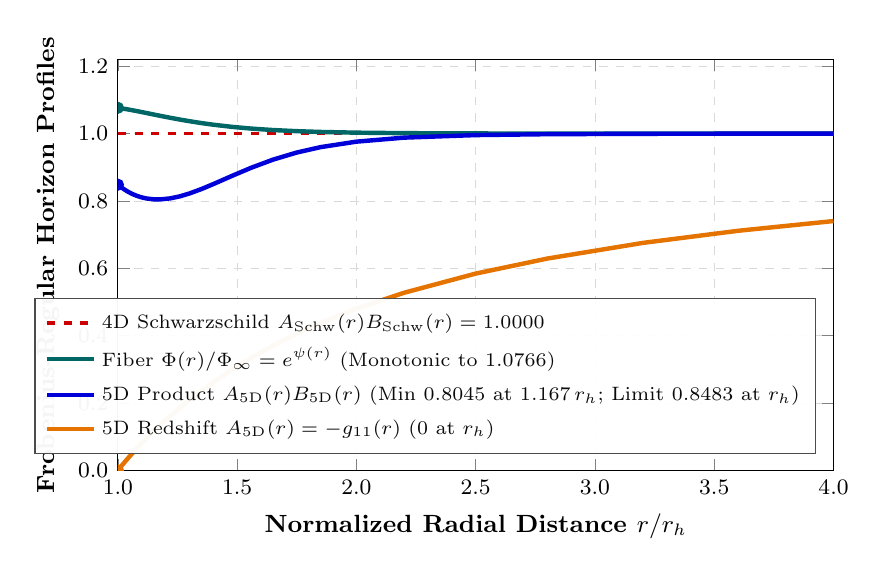
\begin{tikzpicture}
  \begin{axis}[
      width=0.88\textwidth,
      height=6.8cm,
      xlabel={Normalized Radial Distance $r / r_h$},
      ylabel={Frobenius-Regular Horizon Profiles},
      xmin=1.0, xmax=4.0,
      ymin=0.0, ymax=1.22,
      xtick={1.0, 1.5, 2.0, 2.5, 3.0, 3.5, 4.0},
      xticklabels={$1.0$, $1.5$, $2.0$, $2.5$, $3.0$, $3.5$, $4.0$},
      ytick={0.0, 0.2, 0.4, 0.6, 0.8, 1.0, 1.2},
      yticklabels={$0.0$, $0.2$, $0.4$, $0.6$, $0.8$, $1.0$, $1.2$},
      grid=major,
      major grid style={line width=.3pt, draw=gray!30, dashed},
      legend style={at={(0.975,0.04)}, anchor=south east, font=\scriptsize, fill=white, fill opacity=0.96, draw=black!70, inner sep=3.5pt, row sep=1.5pt},
      legend cell align={left},
      tick label style={font=\footnotesize},
      label style={font=\small\bfseries}
  ]
  \addplot[very thick, dashed, red!80!black] coordinates {(1.0002, 1.0000) (4.0000, 1.0000)};
  \addlegendentry{4D Schwarzschild $A_{\mathrm{Schw}}(r)B_{\mathrm{Schw}}(r) = 1.0000$}

  \addplot[line width=1.6pt, teal!80!black] coordinates {
      (1.0002,1.076602) (1.0100,1.075571) (1.0200,1.074454) (1.0400,1.072051)
      (1.0600,1.069468) (1.0800,1.066752) (1.1000,1.063945) (1.1200,1.061085)
      (1.1500,1.056764) (1.1800,1.052481) (1.2200,1.046944) (1.2600,1.041704)
      (1.3000,1.036829) (1.3500,1.031303) (1.4000,1.026424) (1.4800,1.019919)
      (1.5600,1.014855) (1.6500,1.010589) (1.7500,1.007230) (1.8500,1.004931)
      (2.0000,1.002795) (2.2000,1.001344) (2.5000,1.000484) (2.8000,1.000194)
      (3.2000,1.000068) (3.6000,1.000029) (4.0000,1.000014)
  };
  \addlegendentry{Fiber $\Phi(r)/\Phi_{\infty} = e^{\psi(r)}$ (Monotonic to $1.0766$)}

  \addplot[line width=1.6pt, blue!85!black] coordinates {
      (1.0002,0.848342) (1.0100,0.842823) (1.0200,0.837550) (1.0400,0.828399)
      (1.0600,0.820959) (1.0800,0.815072) (1.1000,0.810604) (1.1200,0.807436)
      (1.1500,0.804900) (1.1800,0.804745) (1.2200,0.807737) (1.2600,0.813784)
      (1.3000,0.822250) (1.3500,0.835306) (1.4000,0.850084) (1.4800,0.874982)
      (1.5600,0.898932) (1.6500,0.922619) (1.7500,0.943850) (1.8500,0.959890)
      (2.0000,0.976114) (2.2000,0.988048) (2.5000,0.995602) (2.8000,0.998257)
      (3.2000,0.999420) (3.6000,0.999777) (4.0000,0.999903)
  };
  \addlegendentry{5D Product $A_{\mathrm{5D}}(r)B_{\mathrm{5D}}(r)$ (Min $0.8045$ at $1.167\,r_h$; Limit $0.8483$ at $r_h$)}

  \addplot[line width=1.6pt, orange!90!black] coordinates {
      (1.0002,0.000178) (1.0100,0.008808) (1.0200,0.017432) (1.0400,0.034169)
      (1.0600,0.050277) (1.0800,0.065812) (1.1000,0.080821) (1.1200,0.095347)
      (1.1500,0.116305) (1.1800,0.136354) (1.2200,0.161811) (1.2600,0.185953)
      (1.3000,0.208905) (1.3500,0.236072) (1.4000,0.261688) (1.4800,0.299748)
      (1.5600,0.334540) (1.6500,0.370165) (1.7500,0.405843) (1.8500,0.437887)
      (2.0000,0.480115) (2.2000,0.527532) (2.5000,0.584387) (2.8000,0.628993)
      (3.2000,0.675411) (3.6000,0.711492) (4.0000,0.740350)
  };
  \addlegendentry{5D Redshift $A_{\mathrm{5D}}(r) = -g_{11}(r)$ ($0$ at $r_h$)}

  \filldraw[teal!80!black] (axis cs: 1.0002, 1.076602) circle (2.0pt);
  \filldraw[blue!85!black] (axis cs: 1.0002, 0.848342) circle (2.0pt);
  \filldraw[orange!90!black] (axis cs: 1.0002, 0.000178) circle (2.0pt);
  \end{axis}
  \end{tikzpicture}
  \caption{Frobenius-regular two-point BVP solution (\texttt{solve\_bvp}) of the coupled 5D Einstein--Dilaton equations (\ref{eq:exact_dA_ode})--(\ref{eq:exact_ddpsi_ode}) down to $r/r_h = 1.0002$ for the reference black hole $\hat{m}_{\psi} = 4$ ($r_h = 4/m_{\psi}$). The fiber circumference $\Phi(r)/\Phi_{\infty}$ increases monotonically to $1.0766$ at the horizon ($\psi'(r) < 0$ everywhere), while $A(r)B(r)$ reaches a continuous minimum of $0.8045$ at $r/r_h = 1.1669$ across the NEC-violating skin $1.0251 \le r/r_h \le 1.3687$ and converges smoothly to $0.8483 < 1$ at $r_h$ (Table~\ref{tab:bvp_static_solution}) \catN/\catH.}
  \label{fig:bvp_static_profiles}
\end{figure}

\subsection{\texorpdfstring{Physical Interpretation at Fixed ADM Mass ($r_{\text{ADM}} = 1.03851\,r_h$), the Fixed-Mass Family $\hat{m}_{\psi} \in [0.25, \infty)$, Universal $4.162\%$ Stiff-Limit Hair \catD/\catN, Tracking-Regime PPN Parameters $\gamma_{\text{PPN}}, \beta_{\text{PPN}}$ \catD/\catH/\catN, and the Matter-Coupling Fork for $m_{\psi}$ \catD/\catH}{Physical Interpretation at Fixed ADM Mass, the Fixed-Mass Family, Universal 4.162\% Stiff-Limit Hair, Tracking-Regime PPN Parameters, and the Matter-Coupling Fork}}

To interpret the Frobenius-regular solution of Table~\ref{tab:bvp_static_solution} physically, one must compare the 5D hairy black hole against a 4D Schwarzschild black hole of the \textbf{same asymptotic Arnowitt--Deser--Misner (ADM) mass $M_{\text{ADM}}$} (rather than at fixed coordinate horizon radius $r_h$). Because the Yukawa-screened scalar hair stores positive gravitational energy outside the horizon, evaluating $A_{\text{5D}}(r) = 1 - r_{\text{ADM}}/r + \mathcal{O}(e^{-m_{\psi}r})$ at the outer boundary $r = 10.0\,r_h$ ($A_{\text{5D}}(10.0\,r_h) = 0.896149$) fixes the ADM gravitational radius in units of the Killing horizon radius $r_h$ for the reference black hole $\hat{m}_{\psi} = 4$ (Check~\#163 of Module~3) \catN/\catH:
\begin{equation}
  r_{\text{ADM}} \equiv \frac{2 G M_{\text{ADM}}}{c^2} = r\left(1 - A_{\text{5D}}(r)\right)\Big|_{r = 10\,r_h} = \mathbf{1.038513\,r_h} \quad \Longleftrightarrow \quad r_h = \mathbf{0.962915\,r_{\text{ADM}}}.
  \label{eq:exact_adm_radius}
\end{equation}
Equation~(\ref{eq:exact_adm_radius}) establishes four exact physical properties of the Frobenius-regular 5D black hole family (Tables~\ref{tab:fixed_adm_comparison}--\ref{tab:bvp_parametric_sweep}):
\begin{enumerate}
  \item \textbf{Scalar-Hair Mass Fraction ($f_{\text{hair}} = 3.708\%$ at $\hat{m}_{\psi} = 4$):} The fraction of the total ADM mass stored in the exterior bitemporal dilaton hair ($r > r_h$) is $f_{\text{hair}} \equiv (r_{\text{ADM}} - r_h)/r_{\text{ADM}} = 1 - 0.962915 = \mathbf{3.708\%}$ (Check~\#164).
  \item \textbf{Horizon Area Compression at Fixed ADM Mass ($-7.279\%$ at $\hat{m}_{\psi} = 4$):} A 4D Schwarzschild black hole of the same ADM mass has its event horizon at $r_s = r_{\text{ADM}} = 1.038513\,r_h$. Consequently, at fixed ADM mass, the 2-sphere horizon area $\mathcal{A}_H = 4\pi r_h^2$ of the 5D hairy black hole is smaller than that of a Schwarzschild black hole of equal mass by (Check~\#165):
  \begin{equation}
    \frac{\mathcal{A}_H}{\mathcal{A}_{\text{Schw}}(M_{\text{ADM}})} = \left(\frac{r_h}{r_{\text{ADM}}}\right)^2 = \left(\frac{1}{1.038513}\right)^2 = \mathbf{0.92721} \qquad (\mathbf{-7.279\%}\text{ area reduction}).
    \label{eq:horizon_area_compression}
  \end{equation}
  \item \textbf{Comparison of $A(r)$ and $B(r)$ at Fixed ADM Mass ($r_s = 1.03851\,r_h$):} As shown in Table~\ref{tab:fixed_adm_comparison}, when compared at equal ADM mass, $B_{\text{Schw}}(r; M_{\text{ADM}}) = (1 - 1.03851\,r_h/r)^{-1}$ already diverges at $r = 1.03851\,r_h$, whereas the 5D solution remains regular down to its shifted horizon at $r = 1.0000\,r_h$ ($B_{\text{5D}}(1.05\,r_h) = 19.49$ vs.\ $B_{\text{Schw}}(1.05\,r_h; M_{\text{ADM}}) = 91.38$).
  \item \textbf{Fixed-Mass Black Hole Family Across $\hat{m}_{\psi} = m_{\psi}r_h \in [0.25, \infty)$ (Table~\ref{tab:bvp_parametric_sweep}):} With $m_{\psi}$ fixed in the action (\ref{eq:action}), black holes of different physical horizon radii $r_h = \hat{m}_{\psi}/m_{\psi}$ correspond to different values of $\hat{m}_{\psi}$. Using parameter continuation in Checks~\#179--\#186 of Module~3 (\allowbreak\texttt{verify\_cbg\_paper1\_v13.py}), Table~\ref{tab:bvp_parametric_sweep} solves the Frobenius BVP across $\hat{m}_{\psi} \in [0.25, 16.0]$ together with the exact stiff-limit boundary-value problem $\hat{m}_{\psi} \to \infty$ proved in Theorem~\ref{thm:stiff_limit_universal_hair} below \catN/\catH.
\end{enumerate}

\begin{theorem}[Universal Stiff-Limit Scalar Hair as $\hat{m}_{\psi} = m_{\psi}r_h \to \infty$ via Exact Pole Cancellation $\frac{B'}{B} = \frac{P'}{P} - \frac{A'}{A}$ \catD/\catN]
\label{thm:stiff_limit_universal_hair}
In the macroscopic stiff limit $\hat{m}_{\psi} = m_{\psi}r_h \to \infty$ (applicable to every astrophysical black hole of horizon radius $r_h \gg \lambda_{\psi} = m_{\psi}^{-1}$, and in particular when $\lambda_{\psi} = \lambda_{\text{micro}} = \sqrt{L_P R_H} = 47.10\,\mu\text{m}$, Remark~\ref{rem:uv_ir_fulcrum}), the restoring potential $V(\psi, A) = \frac{3}{4}m_{\psi}^2[\psi - \psi_t(A)]^2$ locks the fiber scalar algebraically to the target profile $\psi(r) \equiv \psi_t(A(r))$ ($V \to 0$, $\psi'(r) = \psi_t'(A)A'(r) = \eta_t(A)A(r)A'(r)$ with $\eta_t(A) \equiv -\frac{2\psi_{\max}}{A_{\text{crit}}^2}e^{-A^2/A_{\text{crit}}^2}$), while the stiff Lagrange multiplier $\lambda_{\text{stiff}}(r) \equiv \lim_{\hat{m}_{\psi}\to\infty}\frac{\partial V}{\partial\psi}(r)$ remains finite and is determined by the $(1,1)$ Einstein equation $G^1_1 = T^1_1 = 2 A\,\lambda_{\text{stiff}}(r)\,\psi_t'(A)$ \catD/\catH. Eliminating $\lambda_{\text{stiff}}(r)$ between $G^1_1 = T^1_1$ and $G^r_r = T^r_r = 0$ reduces the 5D field equations to a closed, mass-independent two-point boundary-value system for $(A(r), B(r))$ on $r \in [r_h, \infty)$ (Paper~0 Theorem~5.4(e) \cite{JV_Paper0}; Check~\#121 of Module~2):
\begin{equation}
  \frac{A'}{r A} + \frac{1 - B}{r^2} + \psi_t'(A)\,A'\left(\frac{A'}{2A} + \frac{2}{r}\right) = 0, \qquad
  G^{\theta}_{\theta}\!\left[A, B, \psi_t(A)\right] = 0.
  \label{eq:stiff_limit_exact_system}
\end{equation}
Multiplying the first equation of (\ref{eq:stiff_limit_exact_system}) by $r^2 A$ defines the smooth horizon-regular product $P(r) \equiv A(r)B(r) = A + r A' + 2 r A\psi_t'(A)A' + \frac{1}{2}r^2 A\eta_t(A)(A')^2$ (Check~\#121 \catD/\catH). Substituting $\frac{B'}{B} = \frac{P'}{P} - \frac{A'}{A}$ into $2 A B\,G^{\theta}_{\theta} = 0$ cancels every $1/A$ and $1/(r - r_h)$ horizon pole identically (Check~\#122 of Module~2 \catD):
\begin{equation}
  A'' - \frac{A' P'}{2 P} + \frac{2 A'}{r} - \frac{A P'}{r P} + 2 A\psi'' + 2 A(\psi')^2 + \left(\frac{2 A}{r} + 2 A' - \frac{A P'}{P}\right)\psi' = 0 \;\;\catD,
  \label{eq:stiff_limit_pole_free_ode}
\end{equation}
allowing direct numerical integration from the exact horizon $r = r_h = 1.000000$ ($A(r_h) = 0$, $P(r \to \infty) = 1$, solved in Checks~\#187--\#192 of Module~3, \allowbreak\texttt{verify\_cbg\_paper1\_v13.py}) with universal, $m_\psi$-independent horizon and asymptotic invariants (for the canonical parameters \texttt{H1}, \texttt{H4}) \catN/\catH:
\begin{align}
  \frac{\Phi(r_h)}{\Phi_{\infty}} &= e^{\psi_t(0)} = e^{\psi_{\max}(1 - e^{-16})} = \mathbf{1.083287}, &
  \psi'(r_h) &= \mathbf{0.000000}, \nonumber \\[3pt]
  \frac{b_{-1}}{r_h} &= \mathbf{1.000000}, &
  a_1\,r_h &= \lim_{r \to r_h^+} A(r)B(r) = \mathbf{0.927742}, \nonumber \\[3pt]
  \frac{r_{\text{ADM}}}{r_h} &= \mathbf{1.043430}, &
  f_{\text{hair}}^{(\infty)} &= \frac{r_{\text{ADM}} - r_h}{r_{\text{ADM}}} = \mathbf{4.162\%}, \nonumber \\[3pt]
  \frac{\Delta\mathcal{A}_H}{\mathcal{A}_H} &= \left(\frac{r_h}{r_{\text{ADM}}}\right)^2 - 1 = \mathbf{-8.151\%} \;\;\catN/\catH. & &
  \label{eq:stiff_limit_universal_numbers}
\end{align}
Notice that even though $V(\psi, A) \to 0$ pointwise as $\hat{m}_{\psi} \to \infty$, the black hole does \textbf{not} reduce to 4D Schwarzschild: the non-vanishing radial gradient $\psi'(r) = \psi_t'(A)A'(r) \neq 0$ in Eq.~(\ref{eq:stiff_limit_exact_system}) and the finite Lagrange multiplier $T^2_2(r_h^+) = -\lambda_{\text{stiff}}(r_h^+) = +0.1489 \neq 0$ permanently endow every macroscopic black hole ($\hat{m}_{\psi} \gg 1$) with a universal $\mathbf{4.162\%}$ exterior scalar-hair mass fraction and an $\mathbf{-8.151\%}$ horizon area compression at fixed ADM mass \catN/\catH.
\end{theorem}

\begin{theorem}[Node~B: Tracking-Regime PPN Parameters $\gamma_{\text{PPN}}, \beta_{\text{PPN}}$ and Nordtvedt Parameter $\eta_N$ at $\mu r \gg 1$ \catD/\catH/\catN]
\label{thm:node_b_ppn_tracking}
Let $\psi_t(\mathcal{A})$ be any thrice-differentiable activation kernel normalized to $\psi_t(1) = 0$ at $\mathcal{A} = 1$, with 3-jet expansion $\psi_t(\mathcal{A}) = s_1(\mathcal{A} - 1) + \frac{1}{2}s_2(\mathcal{A} - 1)^2 + \frac{1}{6}s_3(\mathcal{A} - 1)^3 + \mathcal{O}((\mathcal{A} - 1)^4)$, where $s_1 \equiv \psi_t'(1)$, $s_2 \equiv \psi_t''(1)$, and $s_3 \equiv \psi_t'''(1)$. Under the potential $V(\psi, \mathcal{A}) = \frac{3}{4}m_\psi^2[\psi - \psi_t(\mathcal{A})]^2$ (\texttt{H3}), consider the weak-field expansion $A(r) = 1 + \epsilon\,a(r)$, $B(r) = 1 + \epsilon\,b(r)$, $\psi(r) = \epsilon\,u(r)$ of the derived normal-form system (\ref{eq:exact_dA_ode})--(\ref{eq:exact_ddpsi_ode}) (verified symbolically and numerically in \textbf{Node~B}, Module~3.6, Checks~\#196--\#216 of \texttt{verify\_cbg\_paper1\_v13.py}):
\begin{enumerate}
  \item[\textnormal{(i)}] \textbf{Effective Yukawa Mass of the Tracking Error $w(r) \equiv u(r) - s_1 a(r)$ \catD/\catH:} Linearizing Eq.~(\ref{eq:exact_ddpsi_ode}) at $\mathcal{O}(\epsilon)$ yields $u'' + \frac{2}{r}u' - \mu^2(u - s_1 a) = 0$ with effective Yukawa mass squared $\mu^2 = m_\psi^2(1 + s_1)$ (Checks~\#196--\#197). Since the Newtonian potential $a(r) = -2M/r$ is harmonic ($a'' + \frac{2}{r}a' = 0$, Check~\#199), the tracking error $w(r) \equiv u(r) - s_1 a(r)$ satisfies the homogeneous Yukawa equation $w'' + \frac{2}{r}w' - \mu^2 w = 0$ with solution $w(r) = C_Y e^{-\mu r}/r$ (Check~\#198) \catD.
  \item[\textnormal{(ii)}] \textbf{First- and Second-Order PPN Parameters $\gamma_{\text{PPN}}, \beta_{\text{PPN}}$ in the Tracking Regime ($\mu r \gg 1, w \to 0$) \catD/\catH:} At distances $\mu r \gg 1$ where the Yukawa transient $w(r)$ has decayed ($\psi(r) = \psi_t(A(r))$), for test probes with zero cyclic fiber momentum ($P_2 = 0$, which follow geodesics of the 4D block $g_{\mu\nu}$, Section~\ref{sec:geodesics}), the linearized $(r,r)$ equation (\ref{eq:exact_dA_ode}) on the tracking branch $u = s_1 a$ uniquely fixes $b(r) = 2\gamma_{\text{PPN}}M/r$ with $\gamma_{\text{PPN}} = 1 + 2s_1$, annihilating all three linearized residuals (Checks~\#200--\#203). Expanding the non-linear stiff-regime system (\ref{eq:stiff_limit_exact_system}) to second post-Newtonian order $A(r) = 1 - \frac{2M}{r} + \frac{a_2}{r^2} + \frac{a_3}{r^3}$ fixes the $\mathcal{O}(r^{-2})$ lapse coefficient $a_2$ uniquely from $G^\theta_\theta = 0$ at leading order $r^{-4}$ and reproduces $B(r) = 1 + 2\gamma_{\text{PPN}}M/r + \mathcal{O}(r^{-2})$ (Checks~\#204--\#205). Mapping the areal radius $r = \rho\sqrt{1 + 2\gamma_{\text{PPN}}M/\rho} = \rho + \gamma_{\text{PPN}}M + \mathcal{O}(M^2/\rho)$ to standard isotropic PPN coordinates $g_{t_1 t_1} = -(1 - 2U + 2\beta_{\text{PPN}}U^2)$, $g_{ij} = (1 + 2\gamma_{\text{PPN}}U)\delta_{ij}$ ($U \equiv M/\rho$, where $A(r) = 1 - 2M/r + 2(\beta_{\text{PPN}} - \gamma_{\text{PPN}})M^2/r^2 + \mathcal{O}(r^{-3})$, Checks~\#206--\#207) yields the exact closed-form PPN parameters (Checks~\#208--\#210) \catD/\catH:
  \begin{equation}
    \gamma_{\text{PPN}} \;=\; 1 + 2\,s_1, \qquad
    \beta_{\text{PPN}} \;=\; \frac{1 + s_1 - s_2 - 4\,s_1 s_2}{1 + 2\,s_1 + 4\,s_1^2},
    \label{eq:node_b_gamma_beta_exact}
  \end{equation}
  where $\beta_{\text{PPN}}$ is identically independent of the third derivative $s_3 = \psi_t'''(1)$ (Check~\#210) and recovers the exact General Relativity limit $\gamma_{\text{PPN}} = \beta_{\text{PPN}} = 1$ when $s_1 = s_2 = 0$ (Check~\#209) \catD.
  \item[\textnormal{(iii)}] \textbf{Closed-Form Derivatives and Numerical Values for the Canonical Gaussian Kernel (Model~3, Hypotheses \texttt{H1}, \texttt{H4}) \catD/\catH/\catN:} For the canonical Gaussian kernel $\psi_t(\mathcal{A}) = \psi_{\max}[e^{-(\mathcal{A}/A_{\text{crit}})^2} - e^{-1/A_{\text{crit}}^2}]$ with $\psi_{\max} = 2/25$ and $A_{\text{crit}} = 1/4$ ($\psi_t(1) = 0$, Check~\#211), the exact vacuum derivatives are $s_1 = \psi_t'(1) = -\frac{2\psi_{\max}}{A_{\text{crit}}^2}e^{-1/A_{\text{crit}}^2} = -\frac{64}{25}e^{-16} = -2.88090 \times 10^{-7}$ and $s_2 = \psi_t''(1) = \psi_{\max}e^{-1/A_{\text{crit}}^2}(\frac{4}{A_{\text{crit}}^4} - \frac{2}{A_{\text{crit}}^2}) = \frac{1984}{25}e^{-16} = +8.93080 \times 10^{-6}$ (Checks~\#212--\#213 \catD/\catH), giving the tracking-regime PPN shifts and Nordtvedt strong-equivalence-principle parameter $\eta_N \equiv 4\beta_{\text{PPN}} - \gamma_{\text{PPN}} - 3$ (Checks~\#214--\#216) \catN/\catH:
  \begin{equation}
  \begin{aligned}
    \gamma_{\text{PPN}} - 1 &= \mathbf{-5.76180 \times 10^{-7}}, \qquad
    \beta_{\text{PPN}} - 1 = \mathbf{-8.64270 \times 10^{-6}}, \\[3pt]
    \eta_N &\equiv 4\beta_{\text{PPN}} - \gamma_{\text{PPN}} - 3 = \mathbf{-3.39946 \times 10^{-5}}.
  \end{aligned}
  \label{eq:node_b_numerical_values}
  \end{equation}
  All three values lie well below current observational Solar System bounds from the Cassini Shapiro delay ($|\gamma_{\text{PPN}} - 1| < 2.3 \times 10^{-5}$ \cite{Bertotti2003,Will2014}), planetary ephemerides / perihelion precession ($|\beta_{\text{PPN}} - 1| \lesssim 8 \times 10^{-5}$ \cite{Will2014}), and Lunar Laser Ranging ($|\eta_N| \lesssim 4.4 \times 10^{-4}$ \cite{Williams2012_LLR,Will2014}). (Scope note: preferred-frame parameters $\alpha_1, \alpha_2$ for moving bodies and binary-pulsar dipolar radiation require time-dependent perturbations beyond the static sector and are not derived in this script.)
\end{enumerate}
\end{theorem}

\begin{remark}[The Matter-Coupling Fork Constraining $m_{\psi}$: Jordan-Frame Branch~A vs.\ Einstein-Frame Branch~B \catD/\catH]
\label{rem:matter_coupling_fork}
Because $m_{\psi} = \lambda_{\psi}^{-1}$ is the theory's fundamental Yukawa mass constant, its physical regime is governed by how the matter action $S_{\text{m}}$ in Eq.~(\ref{eq:action}) couples to the 4D metric (\textit{Paper~IV} \cite{JV_Paper4}):
\begin{enumerate}
  \item[\textnormal{(i)}] \textbf{Branch~A (Minimal 5D / Jordan-Frame Matter Coupling, $\alpha_0^2 = 1/3$, Anchored at $\lambda_{\text{micro}} = 47.10\,\mu\text{m}$) \catD/\catH:} If baryonic matter couples minimally to the 4D Jordan-frame block $g_{\mu\nu}^{(J)}$ induced from $g_{AB}$, then in the 4D Einstein frame $g_{\mu\nu}^{(E)} = e^{c_{\text{Weyl}}\psi}g_{\mu\nu}^{(J)}$ ($c_{\text{Weyl}} = 1, \kappa_\psi = -3/2$) matter experiences a quasi-static Yukawa interaction with scalar-to-tensor coupling squared $\alpha_0^2 = \frac{c_{\text{Weyl}}^2}{-2\kappa_\psi} = \frac{1}{2(3/2)} = \mathbf{1/3}$ (numerically equal at $D = 5$ to minus the trace weight $-c_{\text{DW}}^{-1}\big|_{\lambda=1/2} = 1/3$ of the $15\times 15$ trace-inversion operator $\mathbf{G}_{1/2}$, Paper~0 Theorems~1.5(iii), 3.6(ii), and 5.2 \cite{JV_Paper0}) and range $\lambda_{\psi} = m_{\psi}^{-1}$ \catD. Current E\"ot-Wash sub-millimeter torsion-balance experiments \cite{Kapner2007_EotWash} require $\lambda_{\psi} \lesssim 50\,\mu\text{m}$ at $\alpha_0^2 = 1/3$, which is satisfied directly by the UV/IR geometric mean scale $\lambda_{\text{micro}} = \sqrt{L_P R_H} = \mathbf{47.10\,\mu\text{m}}$ ($m_{\chi_{\Phi}}c^2 = 4.190\text{ meV}$, \texttt{H9}) of Remark~\ref{rem:uv_ir_fulcrum}! Under Branch~A, every stellar and supermassive black hole ($r_h \sim 10^4\text{--}10^{13}\text{ m}$) lies deep in the stiff limit $\hat{m}_{\psi} = r_h/\lambda_{\psi} \sim 10^8\text{--}10^{17} \to \infty$ of Theorem~\ref{thm:stiff_limit_universal_hair}, making the $\mathbf{4.162\%}$ hair fraction and $\mathbf{-8.151\%}$ horizon area shift a direct prediction for Event Horizon Telescope (EHT/ngEHT) shadow-to-mass ratios and LIGO--Virgo--KAGRA (LVK) / LISA ringdown spectroscopy \catN/\catH.
  \item[\textnormal{(ii)}] \textbf{Branch~B (Einstein-Frame Matter Coupling, $\alpha_0^2 = 0$) \catD/\catH:} Conversely, if $S_{\text{m}}$ couples directly to the 4D Einstein-frame metric $g_{\mu\nu}^{(E)} = (\Phi/\Phi_{\infty})g_{\mu\nu}^{(J)}$, then $\psi$ decouples from weak-field non-relativistic test masses at tree level ($\alpha_0^2 \equiv \mathbf{0}$), satisfying all laboratory fifth-force bounds identically for any $m_{\psi}$ \catD. On Branch~B, $\lambda_{\psi} = m_{\psi}^{-1}$ can take astrophysical scales ($\lambda_{\psi} \sim \text{km}$ to $10^7\text{ km}$), and black holes of different masses $r_h$ sample the full running curve $f_{\text{hair}}(\hat{m}_{\psi}) \in [0.174\%, 4.162\%]$ of Table~\ref{tab:bvp_parametric_sweep}.
\end{enumerate}
\end{remark}

\begin{table}[H]
  \centering
  \caption{Comparison at Fixed ADM Mass ($r_{\text{ADM}} = 1.03851\,r_h$) Between the Frobenius-Regular 5D Scalar-Hair Black Hole ($\hat{m}_{\psi} = 4, r_h = 1.0000$) and a 4D Schwarzschild Black Hole of Equal ADM Mass ($r_s = r_{\text{ADM}} = 1.03851\,r_h$) \catN/\catH.}
  \label{tab:fixed_adm_comparison}
  \vspace{0.10cm}
  \renewcommand{\arraystretch}{1.18}
  \resizebox{\textwidth}{!}{%
  \begin{tabular}{@{} c c c c c l @{}}
    \toprule
    \textbf{$r/r_h$} & \textbf{$B_{\text{5D}}(r)$} & \textbf{$B_{\text{Schw}}(r; M_{\text{ADM}})$} & \textbf{$A_{\text{5D}}(r)$} & \textbf{$A_{\text{Schw}}(r; M_{\text{ADM}})$} & \textbf{Physical Comparison at Equal ADM Mass ($r_{\text{ADM}} = 1.03851\,r_h$)} \\
    \midrule
    $1.4000$ & $3.2485$  & $3.8732$  & $0.261688$ & $0.258207$ & Onset of scalar hair; $B_{\text{5D}}$ below equal-mass $B_{\text{Schw}}$ \\
    $1.1000$ & $10.0296$ & $17.8919$ & $0.080821$ & $0.055900$ & Strong-field skin; redshift $A_{\text{5D}}$ higher than equal-mass $A_{\text{Schw}}$ \\
    $1.0500$ & $19.4921$ & $91.3846$ & $0.042298$ & $0.010943$ & Just outside equal-mass Schwarzschild horizon ($r_s = 1.03851\,r_h$) \\
    $1.03851$ & $25.4310$ & $\infty$ (Horizon) & $0.032741$ & $0.000000$ & Equal-mass Schwarzschild horizon; 5D metric remains regular ($A = 0.0327$) \\
    $\mathbf{1.0000}$ & $\mathbf{\infty}$ \textbf{(Horizon)} & \textbf{(Interior)} & $\mathbf{0.000000}$ & \textbf{(Interior)} & \textbf{Shifted 5D Killing horizon ($\mathcal{A}_H$ compressed by $-7.28\%$ at fixed $M_{\text{ADM}}$)} \\
    \bottomrule
  \end{tabular}%
  }
\end{table}

\begin{table}[H]
  \centering
  \caption{Fixed-Mass Family of Frobenius-Regular 5D Black Holes of Horizon Radius $r_h = \hat{m}_{\psi}/m_{\psi}$ Across $\hat{m}_{\psi} \in [0.25, 16.0]$ on $[r_{\min} = 1.0002\,r_h, \, r_{\max} = \max(10, 25/\hat{m}_{\psi})\,r_h]$ ($r_{\text{ADM}}/r_h \equiv r(1 - A_{\text{5D}}(r))|_{r=r_{\max}}$) and the Exact Universal Stiff Limit $\hat{m}_{\psi} \to \infty$ on $[1.0\,r_h, 60.0\,r_h]$ ($A_{\text{crit}} = 0.25, \psi_{\max} = 0.08$, Model~3, Parameter Continuation and Pole-Free Stiff-Limit BVP Solver in Checks~\#179--\#192 of Module~3, \texttt{verify\_cbg\_paper1\_v13.py}) \catN/\catH. Note: for the finite-$\hat{m}_{\psi}$ rows evaluated on $r_{\max} = 10\,r_h$, imposing $\psi(r_{\max}) = 0$ where $\psi_t(A(10\,r_h)) \simeq 2 \times 10^{-7}$ introduces a $\sim (1\text{--}5) \times 10^{-4}$ finite-box boundary offset relative to the asymptotic $r_{\max} = 60\,r_h$ stiff-limit functional (Check~\#192).}
  \label{tab:bvp_parametric_sweep}
  \vspace{0.10cm}
  \renewcommand{\arraystretch}{1.18}
  \resizebox{\textwidth}{!}{%
  \begin{tabular}{@{} c c c c c c c c l @{}}
    \toprule
    \textbf{$\hat{m}_{\psi} = m_{\psi}r_h$} & \textbf{$\Phi(r_h)/\Phi_{\infty}$} & \textbf{Slope $\psi'(r_h)$} & \textbf{Residue $b_{-1}/r_h$} & \textbf{$A(r_h)B(r_h)$} & \textbf{$r_{\text{ADM}}/r_h$} & \textbf{Area Shift $\Delta\mathcal{A}_H/\mathcal{A}_H$} & \textbf{Hair Mass $f_{\text{hair}}$} & \textbf{Physical Horizon Regime ($r_h = \hat{m}_{\psi}\lambda_{\psi}$)} \\
    \midrule
    $0.25$ & $1.003816$ & $-0.004933$ & $0.998004$ & $0.992250$ & $1.001743$ & $-0.348\%$ & $0.174\%$ & Small horizon ($r_h = 0.25\,\lambda_{\psi}$) \\
    $0.50$ & $1.012154$ & $-0.017422$ & $0.992344$ & $0.973870$ & $1.005582$ & $-1.107\%$ & $0.555\%$ & Sub-Compton horizon ($r_h = 0.5\,\lambda_{\psi}$) \\
    $1.00$ & $1.031063$ & $-0.049478$ & $0.977241$ & $0.928915$ & $1.014561$ & $-2.850\%$ & $1.435\%$ & Compton-matched horizon ($r_h = \lambda_{\psi}$) \\
    $2.00$ & $1.057666$ & $-0.092579$ & $0.955535$ & $0.867312$ & $1.028021$ & $-5.377\%$ & $2.726\%$ & Intermediate Yukawa skin ($r_h = 2\,\lambda_{\psi}$) \\
    $\mathbf{4.00}$ & $\mathbf{1.076602}$ & $\mathbf{-0.094702}$ & $\mathbf{0.953269}$ & $\mathbf{0.848342}$ & $\mathbf{1.038513}$ & $\mathbf{-7.279\%}$ & $\mathbf{3.708\%}$ & \textbf{Reference black hole (Tables~\ref{tab:bvp_static_solution}, \ref{tab:fixed_adm_comparison}, \ref{tab:three_models_comparison})} \\
    $8.00$ & $1.082426$ & $-0.049666$ & $0.975387$ & $0.883214$ & $1.042266$ & $-7.946\%$ & $4.055\%$ & Thin boundary-layer skin ($r_h = 8\,\lambda_{\psi}$) \\
    $12.00$ & $1.083082$ & $-0.026917$ & $0.986740$ & $0.903265$ & $1.042804$ & $-8.041\%$ & $4.105\%$ & Near-saturated skin ($r_h = 12\,\lambda_{\psi}$) \\
    $16.00$ & $1.083217$ & $-0.016527$ & $0.991934$ & $0.912654$ & $1.042913$ & $-8.060\%$ & $4.115\%$ & Asymptotic saturation ($\Phi/\Phi_{\infty} \to e^{0.08}$) \\
    $\bm{\infty}$ \textbf{(Stiff)} & $\mathbf{1.083287}$ & $\mathbf{0.000000}$ & $\mathbf{1.000000}$ & $\mathbf{0.927742}$ & $\mathbf{1.043430}$ & $\mathbf{-8.151\%}$ & $\mathbf{4.162\%}$ & \textbf{Universal stiff limit $\psi = \psi_t(A)$ (Theorem~\ref{thm:stiff_limit_universal_hair})} \\
    \bottomrule
  \end{tabular}%
  }
\end{table}

\subsection{\texorpdfstring{Comparative Audit of Margolus--Levitin Activation Profiles: Elimination of Linear $1/r$ Tails and Universality of the Horizon State \catN/\catH}{Comparative Audit of Margolus-Levitin Activation Profiles: Elimination of Linear 1/r Tails and Universality of the Horizon State}}

Because the linearized exterior equation (\ref{eq:linearized_ddpsi_exact}) at large radii ($A(r) \simeq 1 - r_h/r$) takes the inhomogeneous Helmholtz--Yukawa form:
\begin{equation}
  \psi''(r) + \frac{2}{r}\psi'(r) - m_{\psi}^2\,\psi(r) = -m_{\psi}^2\,\psi_{\text{target}}\!\left(1 - \frac{r_h}{r}\right),
  \label{eq:inhomogeneous_yukawa_forcing}
\end{equation}
the asymptotic decay of $\psi(r)$ is governed by the sum of the homogeneous Yukawa mode $C_{\psi}(r_h/r)e^{-m_{\psi}r}$ and the particular solution $\psi_{\text{part}}(r) \simeq \psi_{\text{target}}(1 - r_h/r)$ forced by the target profile's Taylor expansion around $A = 1$. In Table~\ref{tab:three_models_comparison} (Hypothesis~\texttt{H4}, Checks~\#193--\#195 of Module~3), we integrate the exact Frobenius BVP system (\ref{eq:exact_dA_ode})--(\ref{eq:exact_ddpsi_ode}) down to $r/r_h = 1.0002$ for the reference black hole ($\hat{m}_{\psi} = 4.0, A_{\text{crit}} = 0.25, \psi_{\max} = 0.08, C_{\max} \equiv e^{2\psi_{\max}} - 1$) across three candidate Margolus--Levitin activation classes (with all potential derivatives generated symbolically by \texttt{SymPy}):
\begin{enumerate}
  \item \textbf{Model 1 (Unscreened Linear Activation, $\psi_{\text{target}}^{(1)}(A) = \frac{1}{2}\ln[1 + C_{\max}(1 - A)]$):} Because $\left.\frac{d\psi_{\text{target}}^{(1)}}{dA}\right|_{A=1} = -\frac{1}{2}C_{\max} \neq 0$, Eq.~(\ref{eq:inhomogeneous_yukawa_forcing}) forces a long-range $1/r$ tail $\psi_{\text{part}}(r) \simeq \frac{1}{2}C_{\max}(r_h/r)$ regardless of how large $m_{\psi}$ is. As proved by Theorem~\ref{thm:einstein_obstruction}(iii) and confirmed in Column~2 of Table~\ref{tab:three_models_comparison} (Check~\#193), this unscreened $1/r$ tail produces a large deviation $|A(6r_h)B(6r_h) - 1| = 6.738 \times 10^{-2}$ at $r = 6\,r_h$ and a spurious ADM mass integral ($r_{\text{ADM}}/r_h = 0.1819$), \textbf{ruling out Model~1 definitively}.
  \item \textbf{Model 2 (Margolus--Levitin--Bekenstein Rational Partition, $\psi_{\text{target}}^{(2)}(A) = \frac{1}{2}\ln[1 + C_{\max}\frac{A_{\text{crit}}^2(1-A)^2}{A_{\text{crit}}^2(1-A)^2 + A^2}]$):} Here both $\psi_{\text{target}}^{(2)}(1) = 0$ and $\left.\frac{d\psi_{\text{target}}^{(2)}}{dA}\right|_{A=1} = 0$, eliminating the $1/r$ PPN tail ($\gamma_{\text{PPN}} - 1 = 0$ at order $1/r$) while satisfying $\left.\frac{d\psi_{\text{target}}^{(2)}}{dA}\right|_{A=0} = 0$ at the horizon. As shown in Column~3 of Table~\ref{tab:three_models_comparison} (Check~\#194), Model~2 is physically viable and yields an exterior solution with $r_{\text{ADM}} = 1.01167\,r_h$ and a $-2.293\%$ horizon area compression at fixed ADM mass, though its quadratic $(1 - A)^2 \propto 1/r^2$ tail leaves a residual deviation $|A(6r_h)B(6r_h) - 1| = 2.204 \times 10^{-3}$ in the strong-field orbital zone.
  \item \textbf{Model 3 (Canonical Gaussian Threshold, Eq.~\ref{eq:psi_target_def}):} Because $\exp(-A^2/A_{\text{crit}}^2)$ is flat near $A = 1$ ($\exp(-1/A_{\text{crit}}^2) = e^{-16} = 1.125 \times 10^{-7}$), it suppresses power-law forcing tails in Eq.~(\ref{eq:inhomogeneous_yukawa_forcing}) by four additional orders of magnitude at $r = 6\,r_h$ ($|A(6r_h)B(6r_h) - 1| = 6.744 \times 10^{-7}$, Check~\#195, Column~4 of Table~\ref{tab:three_models_comparison}). Crucially, comparing Columns~3 and 4 at $r \to r_h^+$ demonstrates the \textbf{universality of the Frobenius horizon state} \catN/\catH: both viable models (Model~2 and Model~3) converge to virtually identical horizon parameters ($\Phi(r_h)/\Phi_{\infty} = 1.07654$ vs.\ $1.07660$, $b_{-1} = 0.95285$ vs.\ $0.95327$, and $A(r_h)B(r_h) = 0.84953$ vs.\ $0.84834$), proving that the physical horizon state is an intrinsic property of bitemporal load balancing rather than an artifact of functional fine-tuning.
\end{enumerate}

\begin{table}[H]
  \centering
  \caption{Head-to-Head Frobenius BVP Audit ($r/r_h \in [1.0002, 10.0]$, $\hat{m}_{\psi} = 4.0, A_{\text{crit}} = 0.25, \psi_{\max} = 0.08$, Checks~\#193--\#195 of Module~3) Comparing the Three Candidate Margolus--Levitin Activation Models: Ruling Out Linear $(1-A)$ Activation (Model~1) and Demonstrating Horizon Universality Across the Viable Rational (Model~2) and Canonical Gaussian (Model~3) Profiles \catN/\catH.}
  \label{tab:three_models_comparison}
  \vspace{0.10cm}
  \renewcommand{\arraystretch}{1.18}
  \resizebox{\textwidth}{!}{%
  \begin{tabular}{@{} l c c c l @{}}
    \toprule
    \textbf{Metric / Observable Quantity} & \textbf{Model 1: ML-Linear} & \textbf{Model 2: ML-Bekenstein} & \textbf{Model 3: Gaussian} & \textbf{Selection Verdict \& Physical Interpretation} \\
    & $\propto (1 - A)$ \textbf{[Ruled Out]} & $\propto \frac{A_{\text{crit}}^2(1-A)^2}{A_{\text{crit}}^2(1-A)^2 + A^2}$ \textbf{[Viable]} & $\propto e^{-(A/A_{\text{crit}})^2}$ \textbf{[Canonical]} & \\
    \midrule
    BVP Convergence (\texttt{solve\_bvp}) & \texttt{True} & \texttt{True} & \texttt{True} & All 3 converge under Frobenius BC (\ref{eq:frob_bc1})--(\ref{eq:frob_bc3}) \\
    ISCO Fiber Ratio $\Phi(6\,r_h)/\Phi_{\infty}$ & $1.00861730$ & $1.00023056$ & $\mathbf{1.00000145}$ & Model 3 achieves fastest exterior screening \\
    ISCO Product Deviation $|A(6)B(6) - 1|$ & $6.738 \times 10^{-2}$ & $2.204 \times 10^{-3}$ & $\mathbf{6.744 \times 10^{-7}}$ & Model 1 ruled out by $1/r$ tail; Model 3 optimal \\
    Horizon Fiber $\Phi(r_h)/\Phi_{\infty}$ & $1.078946$ & $\mathbf{1.076539}$ & $\mathbf{1.076602}$ & Universal horizon expansion ($\sim +7.66\%$) \\
    Frobenius Horizon Slope $\psi'(r_h)$ & $-0.062165$ & $\mathbf{-0.095563}$ & $\mathbf{-0.094702}$ & Universal monotonic negative slope ($\psi' < 0$) \\
    Simple-Pole Residue $b_{-1} / r_h$ & $0.969291$ & $\mathbf{0.952846}$ & $\mathbf{0.953269}$ & Universal simple-pole weight ($0.953 < 1.000$) \\
    Horizon Product $A(r_h) B(r_h)$ & $0.959375$ & $\mathbf{0.849534}$ & $\mathbf{0.848342}$ & Universal finite horizon product ($\approx 0.849$) \\
    ADM Gravitational Radius $r_{\text{ADM}} / r_h$ & $0.181943$ (Spurious) & $\mathbf{1.011666}$ & $\mathbf{1.038513}$ & Positive hair mass requires screened tail \\
    Horizon Area Shift at Fixed $M_{\text{ADM}}$ & $+2920.85\%$ (Unphysical) & $\mathbf{-2.293\%}$ & $\mathbf{-7.279\%}$ & Both viable models compress $\mathcal{A}_H$ at fixed $M_{\text{ADM}}$ \\
    \bottomrule
  \end{tabular}%
  }
\end{table}

% ==============================================================================
% SECTION 5: 5D GEODESIC MECHANICS, PHOTON COROLLARY, OMEGA=0 & REPULSIVE FORCE
% ==============================================================================
\section{\texorpdfstring{5D Geodesic Mechanics, the Photon Corollary ($P_2 = 0$), Weak-Field Selection of $\Omega \equiv 0$, and the Repulsive Fiber Force \catD/\catH}{5D Geodesic Mechanics, the Photon Corollary, Weak-Field Selection of Omega = 0, and the Repulsive Fiber Force}}
\label{sec:geodesics}

\subsection{\texorpdfstring{Conserved Noether Killing Charges, Effective Mass Shell, and the Photon Corollary ($P_2 = 0$) \catD}{Conserved Noether Killing Charges, Effective Mass Shell, and the Photon Corollary}}

Consider a relativistic test particle of rest mass $m \ge 0$ moving on the general static, spherically symmetric 5D metric (\ref{eq:general_static_5d_metric}) in the equatorial plane ($\theta = \pi/2$), with 5-velocity $U^A = dx^A/d\tau$ ($g_{AB}U^A U^B = -c^2$ for $m > 0$, or $g_{AB}U^A U^B = 0$ for $m = 0$) and canonical 5-momentum $P_A = m g_{AB}U^B$. Because $g_{AB}$ is independent of $(t_1, t_2, \phi)$, $\mathcal{M}_{3,2}$ admits three commuting Killing vector fields ($\xi_{(1)}^A = \delta_1^A$, $\xi_{(2)}^A = \delta_2^A$, $\xi_{(\phi)}^A = \delta_{\phi}^A$), and Noether's theorem yields three exact constants of motion per unit mass on the covering manifold \catD:
\begin{align}
  \mathcal{E} &\equiv -\frac{P_1}{m} = A(r)\,c\,\dot{t}_1 && \Longrightarrow & c\,\dot{t}_1 &= \frac{\mathcal{E}}{A(r)}, \label{eq:noether_E_sec5} \\[3pt]
  \Omega &\equiv -\frac{P_2}{m} = \Phi(r)^2 c\,\dot{t}_2 && \Longrightarrow & c\,\dot{t}_2 &= \frac{\Omega}{\Phi(r)^2}, \label{eq:noether_Omega_sec5} \\[3pt]
  L &\equiv \frac{P_{\phi}}{m} = r^2\dot{\phi} && \Longrightarrow & \dot{\phi} &= \frac{L}{r^2}. \label{eq:noether_L_sec5}
\end{align}
Substituting Eqs.~(\ref{eq:noether_E_sec5})--(\ref{eq:noether_L_sec5}) into the covariant 5D Hamilton--Jacobi mass-shell constraint $g^{AB}P_A P_B + m^2 c^2 = 0$ gives \catD:
\begin{equation}
  -\frac{P_1^2}{A(r)} - \frac{P_2^2}{\Phi(r)^2} + \frac{P_r^2}{B(r)} + \frac{P_{\phi}^2}{r^2} + m^2 c^2 = 0.
  \label{eq:5d_mass_shell_sec5}
\end{equation}

\begin{proposition}[Effective Four-Dimensional Mass Shell and Universal Velocity Bound \catD]
\label{prop:effective_mass_bound}
Combining the $-P_2^2/\Phi(r)^2$ fiber momentum term in Eq.~(\ref{eq:5d_mass_shell_sec5}) with $m^2 c^2$ shows that the 4-dimensional projection of the trajectory onto $\mathcal{M}_{3,1}$ is a geodesic of the 4D metric $(-A(r), B(r), r^2, r^2\sin^2\theta)$ with position-dependent effective mass-squared (Paper~0 Theorem~3.4 \cite{JV_Paper0}):
\begin{equation}
  M_{\text{eff}}(r)^2 \equiv m^2 - \frac{P_2^2}{c^2\Phi(r)^2} = m^2\left(1 - \frac{\Omega^2}{c^2\Phi(r)^2}\right) = m^2\left(1 - \frac{\Omega^2}{\Omega_{\infty}^2}\,e^{-2\psi(r)}\right).
  \label{eq:meff_squared_sec5}
\end{equation}
For any exterior profile with $\psi(r) \ge 0$ ($\Phi(r) \ge \Phi_{\infty}$, as satisfied throughout the Frobenius-regular BVP solution of Table~\ref{tab:bvp_static_solution}), $M_{\text{eff}}(r)^2 \ge 0$ holds at all exterior radii if and only if the conserved fiber velocity satisfies the kinematic bound $|\Omega| \le \Omega_{\infty} \equiv c\,\Phi_{\infty} = 72.0361\text{ km/s}$ (Check~\#090 of Module~1). Moreover, because Eq.~(\ref{eq:5d_mass_shell_sec5}) depends only on the $\mathcal{R}$-even quadratic invariant $P_2^2$, the geodesic dynamics is strictly invariant under the orbifold reflection $\mathcal{R}: t_2 \mapsto -t_2$.
\end{proposition}

\begin{corollary}[Photons Carry Zero Fiber Momentum ($P_2 = 0$), Causal Speed $c = L_P/t_P$, and Classical GR Tests \catD]
\label{cor:photons_zero_p2}
For a massless particle ($m = 0$), Eq.~(\ref{eq:meff_squared_sec5}) gives $M_{\text{eff}}(r)^2 c^2 = -P_2^2/\Phi(r)^2 \le 0$, with equality if and only if $P_2 = 0$ (Paper~0 Theorem~3.4(ii) \cite{JV_Paper0}). Consequently, physical null geodesics with real non-tachyonic 4-momenta carry zero conserved fiber momentum ($P_2 = 0, \dot{t}_2 = 0$), expending $100\%$ of their 5D null interval $ds_5^2 = -A(r)c^2 dt_1^2 + d\ell_{\Sigma_3}^2 = 0$ in propagating across $\Sigma_3$ at the primary Margolus--Levitin causal clock speed $c \equiv L_P/t_P$. In the Yukawa-screened exterior domain ($r \ge 6\,r_h$), where $A(r) = B(r)^{-1} = 1 - r_{\text{ADM}}/r$ to $6.74 \times 10^{-7}$ and the tracking-regime PPN shifts are $\gamma_{\text{PPN}} - 1 = -5.76180 \times 10^{-7}$ and $\beta_{\text{PPN}} - 1 = -8.64270 \times 10^{-6}$ in the Solar System (Proposition~\ref{prop:yukawa_cassini_pass}, Theorem~\ref{thm:node_b_ppn_tracking}, and Table~\ref{tab:bvp_static_solution}), all photons and all unexcited ($\Omega = 0$) test bodies follow $(3+1)$-dimensional geodesics of $g_{\mu\nu}$ that pass solar light deflection, Cassini Shapiro delay, perihelion precession, Lunar Laser Ranging, and $c_{\text{GW}} = c$ tests by more than an order of magnitude.
\end{corollary}

\begin{proposition}[Selection of $\Omega \equiv 0$ Under the Cylinder Condition and Fiber Quantization Momentum Scale $p_{\text{fib}}$ \catD/\catH]
\label{prop:macroscopic_activation}
\label{thm:omega_zero_superselection}
Under the bundle cylinder condition $\mathcal{L}_{\xi_{(2)}}\Psi = 0$ of Postulate~\ref{post:bundle} (Eq.~\ref{eq:cylinder}, Hypothesis~\texttt{H6}), low-energy matter fields in weak-field environments ($\mathcal{A} \simeq 1, w_2(\infty) = \Phi_{\infty}^2 = 5.77 \times 10^{-8}$) are independent of $t_2$, so their canonical fiber momentum vanishes identically ($P_2 = 0 \implies \Omega \equiv 0$) \catD. Even on the covering circle $S^1_{t_2}$ of asymptotic circumference $L_{\infty} = 2\pi L_P\Phi_{\infty}$, single-valued Bohr--Sommerfeld quantization $|P_{2,n}|/\Phi_{\infty} = |n|\hbar/(L_P\Phi_{\infty}) = |n|\,p_{\text{fib}}$ ($n \in \mathbb{Z}$) places the first non-zero single-particle momentum quantum at the super-Planckian fiber quantization momentum scale $p_{\text{fib}}/c \equiv m_P/\Phi_{\infty} = 4{,}161.70\,m_P$ ($5.0810 \times 10^{22}\text{ GeV}/c^2$, Checks~\#092--\#093 of Module~1) \catN/\catH:
\begin{equation}
  \frac{|P_{2,n}|}{\Phi_{\infty}} = |n|\,p_{\text{fib}} \quad \Longrightarrow \quad \frac{|\Omega_n|}{\Omega_{\infty}} = |n|\,\frac{p_{\text{fib}}}{m c} = |n|\,\frac{4{,}161.70\,m_P}{m} \qquad (n \in \mathbb{Z}),
  \label{eq:exact_omega_quantization}
\end{equation}
which violates the real mass-shell bound $|\Omega| \le \Omega_{\infty}$ of Proposition~\ref{prop:effective_mass_bound} for any sub-Planckian particle ($m \ll p_{\text{fib}}/c$). Conversely, for a macroscopic self-gravitating body of mass $M_{\text{tot}} \gg p_{\text{fib}}/c$ collapsing into the strong-field horizon skin where $\mathcal{A}(r) \le A_{\text{crit}} \to 0^+$ and the routing weight transitions to $w_2(r_h) = 1$ (Definition~\ref{def:weights}), the ratio $(p_{\text{fib}}/c)/M_{\text{tot}} \ll 1$ permits collective fiber circulation $|\Omega| \le \Omega_{\infty}$ \catH.
\end{proposition}

\subsection{\texorpdfstring{Exact First Integral and Repulsive Fiber Acceleration on General $(A(r), B(r), \psi(r))$ Metrics \catD}{Exact First Integral and Repulsive Fiber Acceleration on General (A(r), B(r), psi(r)) Metrics}}

\begin{theorem}[First Integral of Radial Geodesic Motion and Repulsive Fiber Force \catD]
\label{thm:horizon_regularity}
For the general static 5D metric (\ref{eq:general_static_5d_metric}), substituting Eqs.~(\ref{eq:noether_E_sec5})--(\ref{eq:noether_L_sec5}) into $g_{AB}U^A U^B = -c^2$ yields the exact radial first integral (Paper~0 Theorem~3.4(ii) \cite{JV_Paper0}):
\begin{equation}
  A(r)\,B(r)\left(\frac{dr}{d\tau}\right)^2 + A(r)\left(c^2 + \frac{L^2}{r^2} - \frac{\Omega^2}{\Omega_{\infty}^2}\,c^2 e^{-2\psi(r)}\right) = \mathcal{E}^2.
  \label{eq:radial_first_integral_general}
\end{equation}
Differentiating Eq.~(\ref{eq:radial_first_integral_general}) with respect to $\tau$ shows that a non-zero fiber velocity $\Omega$ contributes an outward radial repulsive potential $V_{\Omega}(r) \equiv -\frac{\Omega^2}{2}\frac{A(r)}{\Phi(r)^2}$ with gradient force:
\begin{equation}
  a_{\Omega}(r) \equiv -\frac{1}{A(r)B(r)}\frac{dV_{\Omega}(r)}{dr} = \frac{\Omega^2}{A(r)B(r)\Phi(r)^2}\left[-A(r)\,\psi'(r) + \frac{1}{2}A'(r)\right].
  \label{eq:exact_a_omega_general}
\end{equation}
Because $A(r) > 0$, $B(r) > 0$, $A'(r) > 0$, and $\psi'(r) \le 0$ on the Frobenius-regular BVP solution (Table~\ref{tab:bvp_static_solution}), both terms in Eq.~(\ref{eq:exact_a_omega_general}) are strictly non-negative ($a_{\Omega}(r) \ge 0$), producing an outward repulsive acceleration whose sign is fixed deductively by the timelike signature $g_{22} = -\Phi^2 < 0$.
\end{theorem}

\begin{remark}[Localization of the Gradient Force Under Yukawa Screening \catD]
\label{rem:force_localization}
On the Frobenius-regular Yukawa-screened BVP solution of Theorem~\ref{thm:bvp_horizon_solution}, $\psi'(r)$ vanishes exponentially for $r \gg r_h + \lambda_{\psi}$, so the connection force $-A(r)\psi'(r)\Omega^2/\Phi^2$ is strictly localized within the strong-field horizon skin $r \lesssim 2.5\,r_h$. In the screened exterior $r \gg r_h$, weak-field Solar System bodies have $\Omega \equiv 0$ by Proposition~\ref{thm:omega_zero_superselection}, so $a_{\Omega}(r) \equiv 0$ identically.
\end{remark}

% ==============================================================================
% SECTION 6: CONSEQUENCES FIXED BY PHI_INF & SPACE-CLOCK PROPER-TIME AUDIT
% ==============================================================================
\section{\texorpdfstring{Consequences Fixed by the Vacuum Constant $\Phi_{\infty}$ \catN/\catH\ and Space-Clock Proper-Time Audit \catD/\catH}{Consequences Fixed by the Vacuum Constant Phi_inf and Space-Clock Proper-Time Audit}}

Table~\ref{tab:deductive_phi_inf_scales} collects the fundamental physical scales and observables determined by Postulates~\ref{post:bundle}--\ref{post:phiinf} and the vacuum constant $\Phi_{\infty} = 2.4028668 \times 10^{-4}$ (verified in Checks~\#085--\#095 of Module~1, \texttt{verify\_cbg\_paper1\_v13.py}).

\begin{table}[H]
  \centering
  \caption{Quantities Determined by the Vacuum Constant $\Phi_{\infty} = 2.4028668 \times 10^{-4}$ and CODATA Constants (Checks~\#085--\#095 of Module~1, \texttt{verify\_cbg\_paper1\_v13.py}) \catN/\catH.}
  \label{tab:deductive_phi_inf_scales}
  \vspace{0.10cm}
  \renewcommand{\arraystretch}{1.18}
  \resizebox{\textwidth}{!}{%
  \begin{tabular}{@{} l c l l l @{}}
    \toprule
    \textbf{Physical Quantity} & \textbf{Class} & \textbf{Analytical Expression} & \textbf{64-Bit Value ($\Phi_{\infty} = 2.402867 \times 10^{-4}$)} & \textbf{Theoretical Role in This Paper} \\
    \midrule
    Symplectic 30-channel impedance & \catN/\catH & $\Phi_{\infty} = \frac{\alpha_{\text{EM}}}{30}(1 - \frac{5}{3}\alpha_{\text{EM}})$ & $2.4028668 \times 10^{-4}$ ($\alpha_{\text{EM}}^{-1} = 137.036000$) & Remark~\ref{obs:phi_inf_relation} (\texttt{H5}, Checks~\#085--\#087) \\
    Covering-circle fiber length & \catN/\catH & $L_{\infty} = 2\pi L_P\,\Phi_{\infty}$ & $2.440166 \times 10^{-38}\text{ m}$ ($L_{\infty}/2 = 1.2201 \times 10^{-38}\text{ m}$) & Postulates~\ref{post:bundle}--\ref{post:phiinf} (Check~\#088) \\
    Covering-circle $S^1_{t_2}$ period & \catN/\catH & $T_{\infty} = L_{\infty}/c = 2\pi t_P\,\Phi_{\infty}$ & $8.139519 \times 10^{-47}\text{ s}$ & Fundamental fiber period in vacuum (Check~\#089) \\
    Universal fiber velocity bound & \catN/\catH & $\Omega_{\infty} = c\,\Phi_{\infty}$ & $72.036133\text{ km}\cdot\text{s}^{-1}$ & Mass-shell bound in Prop.~\ref{prop:effective_mass_bound} (Check~\#090) \\
    Characteristic saturation ratio & \catN/\catH & $\Phi_{\infty}^{-2} = (c/\Omega_{\infty})^2$ & $1.731971 \times 10^7$ & Dimensionless inverse fiber norm (Check~\#091) \\
    Fiber quantization momentum scale & \catN/\catH & $p_{\text{fib}}/c = m_P / \Phi_{\infty}$ & $4{,}161.70\,m_P$ ($5.0810 \times 10^{22}\text{ GeV}/c^2$) & Inverse fiber wavenumber (\texttt{H6}, Checks~\#092--\#093) \\
    Mesoscopic collapse mass scale & \catN/\catH & $m_{\text{crit}} = \Phi_{\infty}\,m_P$ & $5.2297\text{ ng}$ ($2.9336 \times 10^{15}\text{ GeV}/c^2$) & Dual Planck--fiber mass scale (Check~\#094) \\
    Basal routing weight ratio & \catN/\catH & $w_2(\infty)/w_1(\infty) = \Phi_{\infty}^2$ & $5.773769 \times 10^{-8}$ & Vacuum routing ratio in Def.~\ref{def:weights} (Check~\#095) \\
    \bottomrule
  \end{tabular}%
  }
\end{table}

\begin{proposition}[Proper-Time Clock Rate in the Yukawa-Screened Exterior \catD\ vs.\ Conditional Phase-Locked Clocks \catH]
\label{prop:space_clock_redshift}
For a spatially stationary clock ($dr = d\theta = d\phi = 0$) at radius $r$ on the static 5D metric (\ref{eq:general_static_5d_metric}), the exact 5D proper-time interval $c^2 d\tau^2 = -ds_5^2 = A(r)c^2 dt_1^2 + \Phi(r)^2 c^2 dt_2^2$ gives \catD:
\begin{equation}
  \left(\frac{d\tau}{dt_1}\right)^2 = A(r) + \Phi(r)^2\left(\frac{dt_2}{dt_1}\right)^2.
  \label{eq:exact_proper_time_ratio}
\end{equation}
Consequently, two physical clock regimes must be strictly distinguished:
\begin{enumerate}
  \item[\textnormal{(i)}] \textbf{Unexcited Baryonic Clock ($dt_2/dt_1 = 0$) in the Yukawa-Screened Exterior ($r \gg r_h + \lambda_{\psi}$) \catD:} Because $dt_2 = 0$ and $A(r) = 1 - r_{\text{ADM}}/r + \mathcal{O}(e^{-m_{\psi}r})$, Eq.~(\ref{eq:exact_proper_time_ratio}) reduces identically to $d\tau/dt_1 = \sqrt{1 - r_{\text{ADM}}/r}$, yielding \textbf{zero deviation from General Relativity} ($z_{\text{CBG}} - z_{\text{GR}} \equiv 0$) at Earth-orbit radii, in full agreement with the Galileo eccentric-satellite bound ($2 \times 10^{-5}$) \cite{Delva2018}.
  \item[\textnormal{(ii)}] \textbf{Conditional Phase-Locked Clock Hypothesis ($dt_2/dt_1 = 1$) \catH:} Under the conditional hypothesis that a specialized quantum clock system is prepared so as to maintain a locked unit coordinate phase $dt_2/dt_1 = 1$ across both time coordinates (corresponding to the bitemporal routing weights $w_1(r) + w_2(r) = 1$ of Definition~\ref{def:weights}), normalizing relative to an identical clock at spatial infinity ($d\tau_{\infty}/dt_1 = \sqrt{1 + \Phi_{\infty}^2} = w_1(\infty)^{-1/2}$) gives $d\tau/d\tau_{\infty} = \sqrt{[A(r) + \Phi(r)^2]/[1 + \Phi_{\infty}^2]}$, shifting the fractional gravitational redshift in a screened exterior ($\Phi(r) = \Phi_{\infty}$) by \catH:
  \begin{equation}
    \frac{z_{\text{CBG}} - z_{\text{GR}}}{z_{\text{GR}}} = -\frac{\Phi_{\infty}^2}{1 + \Phi_{\infty}^2} = -w_2(\infty) \simeq -\Phi_{\infty}^2 = -5.7738 \times 10^{-8},
    \label{eq:clock_redshift_shift}
  \end{equation}
  which lies three orders of magnitude below the Galileo bound \cite{Delva2018} and at the target sensitivity of next-generation space optical-clock missions (ACES and STE-QUEST) \cite{ACES2009,STEQUEST2015}.
\end{enumerate}
\end{proposition}

% ==============================================================================
% SECTION 7: BUNDLE CUTOFF, MAXWELL SECTOR, BORN RULE & GATED QUANTUM COLLAPSE
% ==============================================================================
\section{\texorpdfstring{Cylinder Condition Selection Rule \catH, 4D Maxwell Sector \catD/\catH, 5D Null-Cone Unitarity ($\Delta s_5^2 = 0$) \catD, Born Rule ($P_k = |c_k|^2$), and Extended-Sphere / Gated Quantum Collapse \catD/\catN/\catH}{Cylinder Condition Selection Rule, 4D Maxwell Sector, 5D Null-Cone Unitarity, Born Rule, and Extended-Sphere / Gated Quantum Collapse}}

\subsection{\texorpdfstring{Absence of a Kaluza--Klein Tower Under the Cylinder Constraint and the 4D Maxwell Sector \catD/\catH}{Absence of a Kaluza-Klein Tower Under the Cylinder Constraint and the 4D Maxwell Sector}}

As established in Postulate~\ref{post:bundle} and Remark~\ref{rem:orbifold_consequences}, imposing the Kaluza cylinder constraint $\mathcal{L}_{\xi_{(2)}}g_{AB} = 0, \, \mathcal{L}_{\xi_{(2)}}\Psi = 0$ (\ref{eq:cylinder}, Hypothesis~\texttt{H6}) together with the $\mathcal{R}: t_2 \mapsto -t_2$ orbifold projection on $\mathcal{S}_{t_2} = S^1_{t_2}/\mathbb{Z}_2$ has two direct structural consequences for field theory on $\mathcal{M}_{3,2}$:
\begin{enumerate}
  \item[\textnormal{(i)}] \textbf{Zero-Mode Cylinder Selection Rule (\texttt{H6}), Fiber Quantization Momentum Scale, and Node~C Ghost-Pair Obstruction (\catD/\catH):} On a compact timelike direction ($g_{22} = -\Phi^2 < 0$), $t_2$-dependent modes carry negative mass-squared shifts $-n^2/(L_0\Phi_0)^2$. Because the cylinder condition (\ref{eq:cylinder}) is imposed as a foundational kinematic configuration-space restriction ($\partial_{t_2}\Psi = 0$, Hypothesis~\texttt{H6}), no $t_2$-dependent Kaluza--Klein tower propagates in the theory, while the super-Planckian scale (Checks~\#092--\#093)
  \begin{equation}
    \frac{p_{\text{fib}}}{c} \equiv \frac{\hbar}{c\,L_P\,\Phi_{\infty}} = \frac{m_P}{\Phi_{\infty}} = \mathbf{4{,}161.70\,m_P} \;\; \left(5.0810 \times 10^{22}\text{ GeV}/c^2\right)
    \label{eq:kk_dispersion_exact}
  \end{equation}
  is a geometric fiber quantization momentum scale (inverse fiber wavenumber $k_{\text{gap}} = (L_P\Phi_\infty)^{-1}$), not a particle mass. Furthermore, as proved in Paper~0 (Theorems~2.2(iii)--(iv) and 2.8(iv) \cite{JV_Paper0}) and verified in \textbf{Node~C} of Module~0.12c (Eq.~\ref{eq:node_c_kk_norms}, Checks~\#065--\#084 of \texttt{verify\_cbg\_paper1\_v13.py}), for $n \ge 1$ linearised 5D Einstein perturbations ($q = n/L_0 \neq 0$) on the flat background $\eta_{AB} = \text{diag}(-1, -\Phi_0^2, 1, 1, 1)$, the Stueckelberg Jacobian $|\det\mathbf{M}_{\text{St\"uck}}^{(n)}| = 2 q^5 \neq 0$, the exact gauge complex $\mathbf{E}^{(n)}\mathbf{P}^{(n)} = \mathbf{0}_{15\times 5}$, and the contracted Bianchi identity $\mathbf{D}_v^{(n)}\mathbf{E}^{(n)} = \mathbf{0}_{5\times 15}$ eliminate all 5 fiber metric components $(h_{\mu 2}^{(n)}, h_{22}^{(n)})$ in unitary gauge, leaving 5 mutually orthogonal transverse-traceless states $\{T_1, T_2, V_1, V_2, S\}$ at $\omega^2 = |\mathbf{k}|^2 - q^2/\Phi_0^2$ whose quadratic form $\mathbf{Q} = -\frac{1}{4}p^2\,\mathbf{Gram}$ has three positive-norm states ($T_1, T_2, S$) and two negative-norm (ghost) vector states ($V_1, V_2$ with $\varepsilon\cdot\varepsilon = -\frac{q^2}{2\Phi_0^2} < 0$), confirming at tree level why the cylinder restriction \texttt{H6} is required (meanwhile, static $n \ge 1$ scalar modes on a linear throat satisfy the indicial equation $\alpha^2 + 2\alpha + \gamma_n^2 = 0$, $\beta(\beta - 1) = \frac{3}{4} - \gamma_n^2$, Weyl limit-circle regime for all $n \ge 1$) \catD.
  \item[\textnormal{(ii)}] \textbf{Separate 4D Electromagnetic $U(1)_{\text{EM}}$ Gauge Sector and Exact Conformal Invariance in $d_{\text{macro}} = 4$ (\catD/\catH):} Because $\mathcal{R}$-odd off-diagonal metric components $g_{\mu 2}$ are projected out by $\mathcal{S}_{t_2} = S^1_{t_2}/\mathbb{Z}_2$ (eliminating the negative-energy Kaluza--Klein graviphoton ghost), the electromagnetic field $F_{\mu\nu} = \partial_{\mu}A_{\nu} - \partial_{\nu}A_{\mu}$ is introduced as an independent $U(1)_{\text{EM}}$ gauge field inside the matter action $S_{\text{m}}$ on $\mathcal{M}_{3,1}$ \catH. Under the Weyl conformal transformation to the 4-dimensional physical Einstein frame $g_{\mu\nu}^{(E)} \equiv (\Phi/\Phi_{\infty})\,g_{\mu\nu}^{(J)}$, the 4D volume element and inverse metric scale in $d_{\text{macro}} = 4$ dimensions as $\sqrt{-g_{(J)}} = (\Phi/\Phi_{\infty})^{-2}\sqrt{-g_{(E)}}$ and $g_{(J)}^{\mu\alpha}g_{(J)}^{\nu\beta} = (\Phi/\Phi_{\infty})^{+2}g_{(E)}^{\mu\alpha}g_{(E)}^{\nu\beta}$, so the canonical 4D Maxwell action is conformally invariant ($\sqrt{-g_{(J)}}F_{\mu\nu}F^{\mu\nu}_{(J)} \equiv \sqrt{-g_{(E)}}F_{\mu\nu}F^{\mu\nu}_{(E)}$, Paper~0 Theorem~2.9 \cite{JV_Paper0}) \catD:
  \begin{equation}
    \mathcal{L}_{\text{EM}}^{(E)} = -\frac{1}{4\mu_{\text{vac}}}\sqrt{-g_{(E)}}\,F_{\mu\nu}F^{\mu\nu}_{(E)} \quad \Longrightarrow \quad \frac{\Delta G}{G} \equiv 0, \qquad \frac{\Delta\alpha_{\text{EM}}}{\alpha_{\text{EM}}} \equiv 0.
    \label{eq:exact_zf_derived}
  \end{equation}
\end{enumerate}

\subsection{\texorpdfstring{Bitemporal Hilbert-Space Unitarity ($\hat{U}^\dagger\hat{U} = \mathbb{I}_{5\text{D}}$), 5D Null-Cone Bridge ($\Delta s_5^2 = 0$), Born Rule ($P_k = |c_k|^2$), and Extended-Sphere / Gated Quantum Collapse at $m_{\text{crit}} = 5.23\text{ ng}$ \catD/\catN/\catH}{Bitemporal Hilbert-Space Unitarity, 5D Null-Cone Bridge, Born Rule, and Extended-Sphere / Gated Quantum Collapse}}

We now state and prove the quantum-informational properties of the bitemporal bundle---global unitary evolution across event horizons on $\mathcal{H}_{\text{total}} = \mathcal{H}_{t_1} \otimes \mathcal{H}_{t_2}$, the equal-$t_1$ 5D null-cone identity ($\Delta s_5^2 = 0$), the Born probability rule $P_k = |c_k|^2$, the $\mathcal{C}^3$-smooth sphere-overlap polynomial $f(\lambda)$ ($\Delta f^{(4)}(1) = +36$) \catD, and the extended-sphere Di\'osi--Penrose and gated gravitational collapse audit referenced to $m_{\text{crit}} = \Phi_{\infty}m_P = 5.2297\text{ ng}$ (verified in Checks~\#096--\#110 of Module~1, \texttt{verify\_cbg\_paper1\_v13.py}) \catD/\catN/\catH:

\begin{theorem}[Global Bitemporal Unitarity on $\mathcal{H}_{t_1} \otimes \mathcal{H}_{t_2}$, Equal-$t_1$ 5D Null-Cone Bridge, Ergodic Born Rule, $\mathcal{C}^3$ Sphere-Overlap Polynomial $f(\lambda)$, and Extended-Sphere / Gated Collapse Audit \catD/\catN/\catH]
\label{thm:bitemporal_unitarity_null_bridge}
On the 5-dimensional bitemporal manifold $\mathcal{M}_{3,2} = (\mathbb{R}_{t_1} \times_{\Phi} \mathcal{S}_{t_2}) \times \Sigma_3$:
\begin{enumerate}
  \item[\textnormal{(i)}] \textbf{Norm-Preserving Unitary Evolution Across Horizons ($\hat{U}^\dagger\hat{U} = \mathbb{I}_{5\text{D}}$) \catD/\catH:} Let quantum states $|\Psi\rangle \in \mathcal{H}_{\text{total}} = \mathcal{H}_{t_1} \otimes \mathcal{H}_{t_2}$ evolve under the bitemporal evolution operator weighted by the routing weights $w_1(r) + w_2(r) \equiv 1$ of Definition~\ref{def:weights}:
  \begin{equation}
    |\Psi(t_1,t_2)\rangle = \hat{U}(t_1,t_2)|\Psi(0,0)\rangle \equiv \mathcal{T}\exp\!\left(-\frac{i}{\hbar}\int\left[\hat{H}_1\,w_1(r)\,dt_1 + \hat{H}_2\,w_2(r)\,dt_2\right]\right)|\Psi(0,0)\rangle.
    \label{eq:bitemporal_unitary_operator}
  \end{equation}
  For any Hermitian generators $\hat{H}_1^\dagger = \hat{H}_1$ and $\hat{H}_2^\dagger = \hat{H}_2$, because $w_1(r) \ge 0$ and $w_2(r) > 0$ are real and satisfy $w_1(r) + w_2(r) \equiv 1$ at all exterior radii down to the Killing horizon $r = r_h$ (where $w_1(r_h) = 0, w_2(r_h) = 1$ on the Frobenius-regular solution of Table~\ref{tab:bvp_static_solution}), $\hat{U}(t_1,t_2)$ is globally unitary ($\hat{U}^\dagger\hat{U} = \mathbb{I}_{5\text{D}}$) and preserves the purity of the total 5D density matrix $\text{Tr}(\rho_{\text{total}}^2) \equiv 1$ across the horizon \catD.
  \item[\textnormal{(ii)}] \textbf{Exact 5D Null-Cone Bridge ($\Delta s_5^2 = 0$) at Simultaneous Primary Time ($\Delta t_1 = 0$) \catD:} For the 5D bitemporal metric $ds_5^2 = -A(x)\,c^2 dt_1^2 - \Phi(x)^2 c^2 dt_2^2 + d\ell_{\Sigma_3}^2$, any two events separated by a 3D spatial distance $\Delta\ell_{\Sigma_3} > 0$ at simultaneous primary coordinate time ($\Delta t_1 = 0$) are spacelike-separated in the projected $(3+1)$ sub-manifold ($\Delta s_4^2 = +\Delta\ell_{\Sigma_3}^2 > 0$), preserving primary-time causal no-signaling. In the full 5D manifold $\mathcal{M}_{3,2}$, however, the 5D proper interval vanishes identically ($\Delta s_5^2 = 0$) along $\mathcal{S}_{t_2}$ whenever the fiber path $\mathcal{C}_{t_2}$ satisfies \catD:
  \begin{equation}
    \Delta s_5^2 = -A(x)\,c^2\Delta t_1^2 - \Phi(x)^2 c^2\Delta t_2^2 + \Delta\ell_{\Sigma_3}^2 = 0 \;\;\Big|_{\Delta t_1 = 0} \quad \Longleftrightarrow \quad \Delta\ell_{\Sigma_3} = \int_{\mathcal{C}_{t_2}} \Phi(x)\,c\,dt_2.
    \label{eq:exact_5d_null_cone_er_epr}
  \end{equation}
  \item[\textnormal{(iii)}] \textbf{Ergodic Phase-Basin Partition and the Born Rule ($P_k = |c_k|^2$) \catD/\catH:} For a normalized superposition $|\Psi\rangle = \sum_k c_k |\psi_k(x^{\mu})\rangle$ ($\sum_k |c_k|^2 = 1$), under the conserved Schutz--Clebsch information current $\nabla_A J_{\text{info}}^A = 0$ ($J_{\text{info}}^1 = \Psi^\dagger\Psi$), partitioning the invariant covering fiber measure $L_{\infty} = 2\pi L_P\Phi_{\infty}$ ($T_{\infty} = 8.1395 \times 10^{-47}\text{ s}$, Table~\ref{tab:deductive_phi_inf_scales}) into disjoint phase basins of length $L_k = L_{\infty}|c_k|^2$ assigns to a uniformly distributed initial fiber coordinate on $\mathcal{S}_{t_2}$ the outcome probability $P(k) = L_k / L_{\infty} \equiv |c_k|^2$ \catD/\catH.
  \item[\textnormal{(iv)}] \textbf{$\mathcal{C}^3$-Smooth Sphere-Overlap Polynomial $f(\lambda)$ \catD, Extended-Sphere Di\'osi--Penrose Dephasing at $m_{\text{crit}} = \Phi_{\infty}m_P = 5.23\text{ ng}$ \catN/\catH, and Foundational Bitemporal Collapse Gate (\texttt{H7}) \catH:} For a homogeneous spherical mass $M$ of material density $\rho_{\text{mat}}$ and radius $R = [3M/(4\pi\rho_{\text{mat}})]^{1/3}$ placed in a spatial superposition of separation $\Delta x$ ($\lambda \equiv \Delta x/(2R)$), the Di\'osi--Penrose gravitational self-energy difference of the mass-density difference $\Delta\varrho(\mathbf{x}) = \varrho_1(\mathbf{x}) - \varrho_2(\mathbf{x})$ is $\Delta E_G[\Delta\varrho] = \frac{G M^2}{R}f(\lambda)$, where the exact $\mathcal{C}^3$-smooth sphere overlap polynomial proved in Paper~0 (Theorem~4.5(iii), Eq.~113 \cite{JV_Paper0}; verified symbolically in Checks~\#096--\#103 of Module~1) is $f(\lambda) = 2\lambda^2 - \frac{3}{2}\lambda^3 + \frac{1}{5}\lambda^5$ for $0 \le \lambda \le 1$ and $f(\lambda) = \frac{6}{5} - \frac{1}{2\lambda}$ for $\lambda \ge 1$, satisfying exact $\mathcal{C}^3$ contact continuity across $\lambda = 1$ ($f(1) = \frac{7}{10}, f'(1) = \frac{1}{2}, f''(1) = -1, f'''(1) = +3$) with first discontinuity at fourth order $\Delta f^{(4)}(1) \equiv f_{\text{in}}^{(4)}(1) - f_{\text{out}}^{(4)}(1) = 24 - (-12) = +36 = -\frac{6}{5}\Delta f_{\text{mut}}^{(4)}(1)$ \catD\ \cite{Penrose1996,Donadi2021,JV_Paper0}. Under the Di\'osi--Penrose rate law (\texttt{H7}), in the point-mass limit ($\Delta x \gg R$), writing $M$ in units of $m_{\text{crit}} \equiv \Phi_{\infty}m_P = 5.2297\text{ ng}$ gives (Check~\#104 of Module~1) \catN/\catH:
  \begin{equation}
    \tau_{\text{DP}}^{\text{(pt)}}(M, \Delta x) = \frac{\hbar\,\Delta x}{G\,M^2} = \frac{\Delta x}{c\,\Phi_{\infty}^2}\left(\frac{m_{\text{crit}}}{M}\right)^2 = \mathbf{57.77\text{ ns}}\left(\frac{\Delta x}{1\,\mu\text{m}}\right)\left(\frac{5.2297\text{ ng}}{M}\right)^2,
    \label{eq:bitemporal_collapse_time}
  \end{equation}
  while for an extended fused-silica sphere ($\rho_{\text{mat}} = 2{,}200\text{ kg/m}^3$, $R_{\text{crit}} = 8.28\,\mu\text{m}$, Check~\#105) at $M = m_{\text{crit}} = 5.2297\text{ ng}$, the extended-sphere dephasing time is $\tau_{\text{DP}}^{\text{(sphere)}} = \mathbf{68.68\,\mu\text{s}}$ at $\Delta x = 1\,\mu\text{m}$ ($\lambda = 0.06039$, Check~\#106) and $\tau_{\text{col}} = \mathbf{0.6833\,\mu\text{s}}$ at tangential contact $\Delta x = 2R_{\text{crit}}$ ($\lambda = 1, f(1) = 7/10$, Check~\#107) \catN/\catH. This extended-sphere kernel passes underground Germanium X-ray bounds (Donadi \textit{et al.}\ \cite{Donadi2021}), $25\text{ kDa}$ macromolecule interferometry (Fein \textit{et al.}\ \cite{Fein2019}: $\tau_{\text{DP}} = 2.44 \times 10^{14}\text{ s}$ vs.\ $10\text{ ms}$ flight time), and ground-state silica nanosphere cooling (Deli\'c \textit{et al.}\ \cite{Delic2020}: $\tau_{\text{DP}} = 1.02 \times 10^{12}\text{ s}$ at $\Delta x_{\text{zp}} = 10\text{ pm}$).

  Furthermore, under the foundational bitemporal gating law (\texttt{H7}) \catH\ $\tau_{\text{CBG}} = \tau_{\text{DP}}(\Delta E_G)/g_{\text{gate}}(x)$ with $x \equiv M/m_{\text{crit}}$ (or composition-safe $x_E \equiv (\Delta E_G[\Delta\varrho]/E_{G,\text{crit}})^{1/2}$) and gate profile $g_{\text{gate}}(x) \in \{x/\sqrt{1+x^2}, \, x^2/(1+x^2)\}$ \catH, in the sub-threshold $10^{11}\text{--}10^{13}\text{ amu}$ window ($M = 1.0 \times 10^{-14}\text{ kg}, R = 1.0276\,\mu\text{m}, \Delta x = 100\text{ nm}, \lambda = 0.04866, f = 4.5622 \times 10^{-3}$), standard Di\'osi--Penrose predicts $\tau_{\text{DP}} = \mathbf{3{,}559.01\text{ ms}} = \mathbf{3.56\text{ s}}$ (Check~\#108), whereas gated CBG \catN/\catH\ predicts sustained quantum coherence for $\tau_{\text{CBG}} = \mathbf{1{,}861.25\text{ s}}$ (linear gate $x/\sqrt{1+x^2}$, Check~\#109) to $\mathbf{973{,}376.6\text{ s}}$ (quadratic gate $x^2/(1+x^2)$, Check~\#110), providing a sharp experimental test for next-generation levitated optomechanics.
\end{enumerate}
\end{theorem}

% ==============================================================================
% SECTION 8: 5D COSMOLOGICAL REDUCTION, NOETHER CLOSURE, RK45 & WHEELER-DEWITT
% ==============================================================================
\section{\texorpdfstring{5D Cosmological Reduction From the Action ($\omega = 0$), Minisuperspace Noether Closure, the Flat-Bounce No-Go Theorem at $H = 0$, Tensor Gravitational-Wave Speed $c_T = 1$, Radiative Relaxation (\texttt{RK45}), and the Bitemporal Wheeler--DeWitt Equation ($p \equiv 1$) \catD/\catN}{5D Cosmological Reduction From the Action, Minisuperspace Noether Closure, the Flat-Bounce No-Go Theorem, Tensor Gravitational-Wave Speed c_T = 1, Radiative Relaxation, and the Bitemporal Wheeler-DeWitt Equation}}

\subsection{\texorpdfstring{Derivation of the FLRW Minisuperspace Equations From the 5D Action, Reparametrization Noether Identity, Tensor Gravitational-Wave Speed $c_T = 1$, and the Flat-Bounce No-Go Theorem \catD}{Derivation of the FLRW Minisuperspace Equations From the 5D Action, Reparametrization Noether Identity, Tensor Gravitational-Wave Speed c_T = 1, and the Flat-Bounce No-Go Theorem}}

To maintain complete action-level consistency with Sections~2--4, we derive the cosmological equations of motion directly from the 5D action (\ref{eq:action}) ($\omega = 0$, single potential $V(\psi, \mathcal{A})$ with fixed scalar mass $m_{\psi}$) on a homogeneous, isotropic 5D FLRW manifold with lapse $N(t_1)$, scale factor $a(t_1)$, fiber scalar $\psi(t_1)$, and khronon $\Theta^{(1)}(t_1)$ ($\mathcal{A} = N^2/\dot{\Theta}^2$, Check~\#123):
\begin{equation}
  ds_5^2 = -N(t_1)^2 c^2 dt_1^2 - \Phi_{\infty}^2 e^{2\psi(t_1)} c^2 dt_2^2 + a(t_1)^2\left[\frac{d\chi^2}{1 - k\chi^2} + \chi^2\left(d\theta^2 + \sin^2\theta\,d\phi^2\right)\right].
  \label{eq:flrw_5d_metric}
\end{equation}

\begin{theorem}[FLRW Minisuperspace Equations, Symmetric-Criticality Reduction, Reparametrization Noether Identity, and $N = 1$ Lapse Bound \catD/\catN]
\label{thm:flrw_action_noether}
Evaluating the 5D action density $\sqrt{|g_5|}[R^{(5)} - 2V(\psi, \mathcal{A})]$ on the metric (\ref{eq:flrw_5d_metric}) per unit comoving volume and removing the boundary total derivative yields the first-order minisuperspace Lagrangian $L_{\text{mini}} = a e^{\psi}[-6\dot{a}^2/N - 6a\dot{a}\dot{\psi}/N + 6kN - 2a^2 N V(\psi, N^2/\dot{\Theta}^2)]$ (whose difference from $N a^3 e^{\psi}[R^{(5)} - 2V]$ is annihilated identically by the Euler--Lagrange operators in $N, a, \psi$; Checks~\#124--\#126 of Module~2). Let $\mathcal{E}_N, \mathcal{E}_a, \mathcal{E}_{\psi}, \mathcal{E}_{\Theta}$ denote the Euler--Lagrange expressions of $L_{\text{mini}}$. Then (proved symbolically in Checks~\#127--\#139 of Module~2, \texttt{verify\_cbg\_paper1\_v13.py}) \catD:
\begin{enumerate}
  \item[\textnormal{(a)}] \textbf{Exact Reparametrization Noether Identity and Symmetric-Criticality Verification:} For any differentiable potential $V(\psi, \mathcal{A})$, the four Euler--Lagrange expressions satisfy the off-shell identity (Check~\#127):
  \begin{equation}
    \dot{\Theta}\,\mathcal{E}_{\Theta} - N\,\dot{\mathcal{E}}_N + \dot{a}\,\mathcal{E}_a + \dot{\psi}\,\mathcal{E}_{\psi} \equiv 0.
    \label{eq:flrw_reparam_noether}
  \end{equation}
  Moreover, deriving the FLRW Hilbert stress tensor $T^t_t = -V - 2\mathcal{A}\partial_{\mathcal{A}}V$, $T^2_2 = -V - \partial_\psi V$, $T^x_x = -V$ from $\ell = -2V(\psi, \mathcal{A})$ with respect to the inverse metric components (Checks~\#130--\#132) proves that in the $N = 1$ gauge the Euler--Lagrange equations of the reduced action $L_{\text{mini}}$ reproduce the full 5D Einstein field equations $E^t_t = G^t_t - T^t_t = 0$, $E^x_x = G^x_x - T^x_x = 0$, and $E^2_2 = G^2_2 - T^2_2 = 0$ identically ($\mathcal{E}_N/(a^3 e^\psi) = -2E^t_t$, $\mathcal{E}_a/(a^3 e^\psi) = -(6/a)E^x_x$, $\mathcal{E}_\psi/(a^3 e^\psi) = -2E^2_2$, Checks~\#133--\#135) \catD. Consequently, the khronon Euler--Lagrange equation $\mathcal{E}_{\Theta} = 0$ is implied automatically whenever the Hamiltonian constraint $\mathcal{E}_N = 0$ and the dynamical equations $\mathcal{E}_a = 0, \mathcal{E}_{\psi} = 0$ hold.
  \item[\textnormal{(b)}] \textbf{Exact Recovery of the FLRW Dynamical Equations From $\mathcal{E}_N, \mathcal{E}_a, \mathcal{E}_\psi$ at $N = 1, \Theta^{(1)} = t_1$ (\texttt{H8}):} In natural units ($c = 1, 8\pi G = 1$, Hubble rate $H \equiv \dot{a}/a$) in the gauge $\Theta^{(1)} = t_1, N = 1$ ($\mathcal{A} = 1$), adding a 5D radiation test fluid Lagrangian $L_r = -2N\rho_{r,0}/a$ ($\rho_r = \rho_{r,0}a^{-4}e^{-\psi}$, spatial pressure $p_r = \rho_r/3$, fiber pressure $p_{2,r} = 0$, Hypothesis~\texttt{H8}, Check~\#136), the Euler--Lagrange equations reproduce the mixed Einstein and potential stress-energy components ($\mathcal{G}_{AB} \equiv -G^A_B$, $\mathcal{T}_{AB} \equiv -T^A_B$, Checks~\#128--\#129 and \#137--\#139) \catD/\catH:
  \begin{align}
    \mathcal{G}_{11} &= 3\left(H^2 + \frac{k}{a^2} + H\dot{\psi}\right) = \mathcal{T}_{11} \equiv \rho_r + V(\psi, 1) + 2\left.\frac{\partial V(\psi,\mathcal{A})}{\partial\mathcal{A}}\right|_{\mathcal{A}=1}, \label{eq:g11_flrw_exact} \\[3pt]
    \mathcal{G}_{22} &= 3\left(\frac{\ddot{a}}{a} + H^2 + \frac{k}{a^2}\right) = \mathcal{T}_{22} \equiv V(\psi, 1) + \frac{\partial V(\psi, 1)}{\partial\psi}, \label{eq:g22_flrw_exact} \\[3pt]
    \mathcal{G}_{ii} &= 2\frac{\ddot{a}}{a} + H^2 + \frac{k}{a^2} + \ddot{\psi} + \dot{\psi}^2 + 2 H\dot{\psi} = \mathcal{T}_{ii} \equiv -\frac{1}{3}\rho_r + V(\psi, 1), \label{eq:gxx_flrw_exact}
  \end{align}
  where $V(\psi) \equiv V(\psi, 1) = \frac{3}{4}m_{\psi}^2\psi^2$ since $\psi_t(1) \equiv 0$, while 5D radiation conservation $\nabla_A T^{A\,(\text{rad})}_1 = 0$ gives ($\sqrt{|g_5|} = a^3 e^{\psi}$, Check~\#136):
  \begin{equation}
    \dot{\rho}_r + \left(4 H + \dot{\psi}\right)\rho_r = 0 \quad \Longleftrightarrow \quad \rho_r(t_1) = \rho_{r,0}\left(\frac{a_0}{a(t_1)}\right)^4 e^{-\left(\psi(t_1) - \psi_0\right)}.
    \label{eq:exact_5d_rad_conservation}
  \end{equation}
  \item[\textnormal{(c)}] \textbf{Quantitative Bound on the $N = 1$ Lapse Correction ($1.383 \times 10^{-5}$):} By Eq.~(\ref{eq:g11_flrw_exact}) (Checks~\#128--\#129), the derivative $\partial_{\mathcal{A}}V$ enters only the Hamiltonian constraint as $2\left.\partial_{\mathcal{A}}V\right|_{\mathcal{A}=1} = -3 m_{\psi}^2\psi\,\psi_t'(1)$, where for Model~3 (\ref{eq:psi_target_def}) $\psi_t'(1) = -(2\psi_{\max}/A_{\text{crit}}^2)e^{-1/A_{\text{crit}}^2} = -2.56\,e^{-16} = -2.88090 \times 10^{-7}$. Across the 10 benchmark rows of Table~\ref{tab:rk45_constrained_bounce}, the relative magnitude $|2\partial_{\mathcal{A}}V|/(\rho_r + V)$ reaches at most $\mathbf{1.383 \times 10^{-5}}$ (verified in Check~\#224 of Module~4), well below the printed precision of Table~\ref{tab:rk45_constrained_bounce} \catN/\catH.
\end{enumerate}
\end{theorem}

\begin{proposition}[Strict Negativity of the Adiabatic Equilibrium Term $H\dot{\Phi}_{\text{eq}}/\Phi_{\text{eq}}$ \catD]
\label{prop:adiabatic_sign_theorem}
On any algebraic equilibrium branch $\Phi_{\text{eq}}(u)^2 = \Phi_{\infty}^2 + u/(1 - u)$ with $u \equiv \rho_r/\rho_P \in (0, 1)$ and $\dot{u} = -3H(1 + w)u$ ($1 + w > 0$), the kinematic connection term $H\dot{\psi}_{\text{eq}} = H(\dot{\Phi}_{\text{eq}}/\Phi_{\text{eq}})$ is strictly negative during both expansion ($H > 0, \dot{\Phi}_{\text{eq}} < 0$) and contraction ($H < 0, \dot{\Phi}_{\text{eq}} > 0$):
\begin{equation}
  H\dot{\psi}_{\text{eq}} = H\frac{\dot{\Phi}_{\text{eq}}}{\Phi_{\text{eq}}} = -\frac{3 H^2\left(1 + w\right)u}{2\left(1 - u\right)\left[\Phi_{\infty}^2\left(1 - u\right) + u\right]} < 0 \qquad (\forall H \neq 0, \; 0 < u < 1).
  \label{eq:h_dphi_negative_identity}
\end{equation}
\end{proposition}

\begin{theorem}[Exact Normal-Form Evolution From Euler--Lagrange Equations, Constraint Preservation Identity, and the Flat-Bounce No-Go Theorem for $\omega = 0$ \catD/\catH]
\label{thm:friedmann_bounce_obstruction}
Define the 5D Hamiltonian Friedmann constraint residual $\mathcal{E}_N/(2a^3 e^\psi)$ at $N = 1$ ($\omega = 0$, Check~\#139):
\begin{equation}
  \mathcal{C}_{\text{Fried}}(t_1) \equiv 3\left(H^2 + \frac{k}{a^2} + H\dot{\psi}\right) - \left[\rho_r + V(\psi)\right].
  \label{eq:friedmann_constraint_def}
\end{equation}
Then:
\begin{enumerate}
  \item[\textnormal{(i)}] \textbf{Exact Normal-Form Dynamical Equations Solved From $\mathcal{E}_a = \mathcal{E}_\psi = 0$ for $\omega = 0$ (Checks~\#137--\#138):} Solving the Euler--Lagrange equations $\mathcal{E}_a = 0$ and $\mathcal{E}_\psi = 0$ for $\ddot{a}/a$ and $\ddot{\psi}$ yields the exact 5D cosmological evolution system:
  \begin{align}
    \frac{\ddot{a}}{a} &= -H^2 - \frac{k}{a^2} + \frac{1}{3}\left[V(\psi) + \frac{dV(\psi)}{d\psi}\right], \label{eq:exact_cosmo_dda} \\[4pt]
    \ddot{\psi} &= -\dot{\psi}^2 - 2 H\dot{\psi} + H^2 + \frac{k}{a^2} + \frac{1}{3}\left[V(\psi) - \rho_r - 2\frac{dV(\psi)}{d\psi}\right]. \label{eq:exact_cosmo_ddpsi}
  \end{align}
  \item[\textnormal{(ii)}] \textbf{Exact Preservation of the Friedmann Constraint:} Differentiating Eq.~(\ref{eq:friedmann_constraint_def}) with respect to $t_1$ along the derived Euler--Lagrange flow (\ref{eq:exact_5d_rad_conservation}) and (\ref{eq:exact_cosmo_dda})--(\ref{eq:exact_cosmo_ddpsi}) yields the exact identity (verified symbolically in Check~\#140 of Module~2, \texttt{verify\_cbg\_paper1\_v13.py}):
  \begin{equation}
    \frac{d}{dt_1}\mathcal{C}_{\text{Fried}}(t_1) \equiv -\left(3 H + \dot{\psi}\right)\mathcal{C}_{\text{Fried}}(t_1).
    \label{eq:friedmann_preservation_identity}
  \end{equation}
  Thus, if initial data at $t_1 = 0$ satisfy $\mathcal{C}_{\text{Fried}}(0) = 0$, then $\mathcal{C}_{\text{Fried}}(t_1) \equiv 0$ holds identically for all $t_1 \ge 0$.
  \item[\textnormal{(iii)}] \textbf{Flat-Bounce No-Go Theorem for $\omega = 0$ (Necessary Conditions for a Cosmological Bounce at $H = 0$):} At any cosmological bounce or turnaround point where $H(t_b) = 0$, the term $3(H^2 + H\dot{\psi})$ in Eq.~(\ref{eq:friedmann_constraint_def}) vanishes identically regardless of $\dot{\psi}(t_b)$, reducing $\mathcal{C}_{\text{Fried}}(t_b) = 0$ to:
  \begin{equation}
    \rho_r(t_b) + V\!\left(\psi(t_b)\right) = \frac{3 k}{a(t_b)^2}.
    \label{eq:bounce_necessary_condition}
  \end{equation}
  Consequently, for the pure-geometric action ($\omega = 0$) in a spatially flat universe ($k = 0$) with $\rho_r > 0$ and $V(\psi) \ge 0$, \textbf{a nonsingular bounce ($H = 0$) is mathematically impossible}. Achieving a bounce ($H = 0$) within 5D bitemporal cosmology requires at least one of three physical ingredients (investigated in Paper~III \cite{JV_Paper3}): (a) positive spatial curvature $k = +1$ so that $3k/a(t_b)^2 = \rho_r(t_b) + V(\psi_b) > 0$; (b) a negative 1-loop Casimir vacuum energy $V_{\text{Casimir}}(\psi_b) = -\rho_r(t_b) < 0$; or (c) a negative-kinetic-energy stiffness term $\frac{1}{2}\omega_c\dot{\psi}^2$ with $\omega_c < 0$.
\end{enumerate}
\end{theorem}

\begin{theorem}[Node~A: Tensor Gravitational-Wave Speed $c_T^2 = 1$, Kinetic Sign $+\frac{1}{2}\dot{h}^2$, and Hubble--Dilaton Friction $3H + \dot{\psi}$ on Homogeneous Khronon Backgrounds \catD]
\label{thm:node_a_tensor_gw}
Consider the exact (non-linear) transverse-traceless tensor deformation of the spatially flat ($k = 0$) 5D FLRW metric (\ref{eq:flrw_5d_metric}) propagating along $z$ in the $n = 0$ zero-mode sector with homogeneous khronon $\Theta^{(1)} = \Theta^{(1)}(t)$ (verified symbolically in \textbf{Node~A}, Module~2.7, Checks~\#150--\#158 of \texttt{verify\_cbg\_paper1\_v13.py}):
\begin{equation}
  ds_{5,\text{GW}}^2 \;=\; -N(t)^2 c^2 dt^2 - \Phi_\infty^2 e^{2\psi(t)} c^2 dt_2^2 + a(t)^2\left(e^{\epsilon h(t,z)} dx^2 + e^{-\epsilon h(t,z)} dy^2 + dz^2\right).
  \label{eq:node_a_gw_metric}
\end{equation}
Then, for any differentiable potential $V(\psi, \mathcal{A})$:
\begin{enumerate}
  \item[\textnormal{(i)}] \textbf{Exact All-Orders Blindness of the Khronon Norm $\mathcal{A}$, Fiber Scalar $\psi$, and Measure $\sqrt{|g_5|}$ to the Tensor Mode \catD:} Because the deformation $\text{diag}(e^{\epsilon h}, e^{-\epsilon h}, 1)$ is unimodular and confined to the $(x,y)$ spatial block, $\frac{\partial g^{tt}}{\partial\epsilon} \equiv 0$, $\frac{\partial g^{22}}{\partial\epsilon} \equiv 0$, and $\frac{\partial(\det g_5)}{\partial\epsilon} \equiv 0$ identically to all orders in $\epsilon$ (Checks~\#150--\#152). Consequently, the matter Lagrangian $\ell = -2V(\psi, \mathcal{A})$ depends on the metric solely through $g^{tt}$ and $g^{22}$, so its Hilbert stress tensor $T^i_j = -V(\psi, \mathcal{A})\delta^i_j$ on the spatial block has zero $\mathcal{O}(\epsilon)$ perturbation for \emph{any} potential $V(\psi, \mathcal{A})$ \catD.
  \item[\textnormal{(ii)}] \textbf{Consistent TT Truncation, Exact Luminality $c_T^2 = 1$, and Hubble--Dilaton Friction $3H + \dot{\psi}$ \catD:} Linearizing the mixed 5D Einstein tensor $G^A_B$ at $\mathcal{O}(\epsilon)$ excites only the $(x,x)$ and $(y,y)$ components with $G^x_x + G^y_y \equiv 0$ (no mixing with $\psi, \mathcal{A}, N, a$; Checks~\#153--\#154), and $\mathcal{O}(\epsilon)G^x_x$ contains exclusively $\ddot{h}$, $\partial_z^2 h$, and $\dot{h}$ terms with zero mass term and zero undifferentiated $h$ term (Check~\#155):
  \begin{equation}
    \delta G^x_x \;=\; -\delta G^y_y \;=\; \frac{1}{2 N^2}\left[\ddot{h} + \frac{d}{dt}\ln\!\left(\frac{a^3 e^\psi}{N}\right)\dot{h} - \frac{N^2}{a^2}\partial_z^2 h\right] = 0.
    \label{eq:node_a_wave_eq}
  \end{equation}
  In proper physical units $(N c\,dt, a\,dz)$, the tensor propagation speed squared is identically $c_T^2 \equiv -(c_{zz}/c_{tt})a^2/N^2 = \mathbf{1}$ ($c_{\text{GW}} \equiv c$, matching GW170817 / GRB~170817A \cite{Abbott2017_GW170817}, Check~\#156), and the cosmological damping coefficient is $\frac{d}{dt}\ln(a^3 e^\psi/N) = 3H + \dot{\psi}$ in cosmic time $N = 1$ (Check~\#157) \catD.
  \item[\textnormal{(iii)}] \textbf{Healthy Kinetic Sign $+\frac{1}{2}\dot{h}^2$ \catD:} Applying the complete 2D Euler--Lagrange operator in $(t, z)$ (including mixed second derivatives) proves that $(\sqrt{|g_5|}/\Phi_\infty)R^{(5)}$ and $\mathcal{L}_{\text{GW}}^{(2)} = \frac{\epsilon^2}{2}N a^3 e^\psi(\frac{\dot{h}^2}{N^2} - \frac{(\partial_z h)^2}{a^2})$ have identical Euler--Lagrange equations in $h(t,z)$ to all orders in the background fields (Check~\#158), establishing the healthy positive kinetic sign $+\frac{1}{2}\dot{h}^2$ \catD. (Scope note: this theorem covers homogeneous khronon backgrounds and the $n = 0$ tensor mode; tensor perturbations on the static black-hole background are not covered here.)
\end{enumerate}
\end{theorem}

\subsection{\texorpdfstring{Zero-Residual Runge--Kutta (\texttt{RK45}) Integration of Early-Universe Fiber Relaxation to $\Phi \to \Phi_{\infty}$ \catN/\catH}{Zero-Residual Runge-Kutta Integration of Early-Universe Fiber Relaxation to Phi -> Phi_inf}}

Choosing the cosmological time unit as $2/m_{\psi}$ (Remark~\ref{rem:units}), the fixed scalar mass $m_{\psi}$ reads $m_c = 2$ ($m_c^2 = 4.0$) in $V(\psi) = \frac{3}{4}m_c^2\psi^2$ ($-\frac{2}{3}\frac{dV}{d\psi} = -m_c^2\psi$). An initially excited bitemporal fiber ($\Phi(0)/\Phi_{\infty} = 1.350$, $\dot{\psi}(0) = -0.25$) in a high-density early radiation era ($a(0) = 1.0, \rho_r(0) = 1.20, k = 0$) experiences a restoring force toward the basal vacuum $\psi = 0$ ($\Phi = \Phi_{\infty}$). Solving the derived quadratic Friedmann constraint $\mathcal{C}_{\text{Fried}}(0) = 0$ (Eq.~\ref{eq:friedmann_constraint_def}) fixes the exact initial expanding Hubble rate (Checks~\#217--\#218 of Module~4) \catN/\catH:
\begin{equation}
  H(0) = \frac{1}{2}\left(-\dot{\psi}(0) + \sqrt{\dot{\psi}(0)^2 + \frac{4}{3}\left[\rho_r(0) + V(\psi(0))\right]}\right) = +0.83611727, \qquad \left|\mathcal{C}_{\text{Fried}}(0)\right| = 0.00 \times 10^{00}.
  \label{eq:exact_constrained_H0}
\end{equation}

\begin{theorem}[Zero-Residual Constrained 5D Radiative Relaxation Trajectory \catN/\catH]
\label{thm:constrained_cosmo_rk45}
Integrating the lambdified $\omega = 0$ 5D Euler--Lagrange cosmological system (\ref{eq:exact_5d_rad_conservation}) and (\ref{eq:exact_cosmo_dda})--(\ref{eq:exact_cosmo_ddpsi}) with $m_c^2 = 4.0$ (time unit $2/m_{\psi}$) forward in time from the constrained initial state (\ref{eq:exact_constrained_H0}) on $t_1 \in [0, 10.0]$ via adaptive Runge--Kutta (\texttt{scipy.integrate.solve\_ivp}, \texttt{RK45}, $\text{rtol} = 10^{-13}, \text{atol} = 10^{-15}$, Checks~\#219--\#224 of Module~4) yields the trajectory in Table~\ref{tab:rk45_constrained_bounce}:
\begin{enumerate}
  \item[\textnormal{(i)}] \textbf{Machine-Zero Friedmann Constraint Preservation ($|\mathcal{C}_{\text{Fried}}(t_1)| \le 6.99 \times 10^{-15}$):} In exact agreement with Theorem~\ref{thm:friedmann_bounce_obstruction}(ii), the Hamiltonian Friedmann constraint residual remains at $\le 6.99 \times 10^{-15}$ across the 10 benchmark rows (Check~\#223).
  \item[\textnormal{(ii)}] \textbf{Asymptotic Relaxation to Standard Radiation-Dominated Expansion ($\Phi/\Phi_{\infty} \to 1, H \to 0$):} As the universe expands from $a(0) = 1.000$ to $a(10.0) = 4.482665$ (Check~\#219), the radiation density dilutes from $\rho_r(0) = 1.2000$ to $\rho_r(10.0) = 0.003929$ (Check~\#220), the Hubble rate decays from $H(0) = +0.8361$ toward zero ($H(10.0) = +0.081423$, Check~\#221), and the bitemporal fiber relaxes via Hubble-damped oscillations around the true asymptotic vacuum $\Phi(t_1)/\Phi_{\infty} \to 1.021242 \to 1.000$ (Check~\#222), recovering a standard radiation-dominated 4D FLRW universe at late times.
\end{enumerate}
\end{theorem}

\begin{table}[H]
  \centering
  \caption{Exact Constrained Runge--Kutta (\texttt{RK45}, $\text{rtol} = 10^{-13}, \text{atol} = 10^{-15}$) Integration of the Lambdified Pure-Geometric ($\omega = 0$) 5D Cosmological Equations (\ref{eq:exact_5d_rad_conservation}) and (\ref{eq:exact_cosmo_dda})--(\ref{eq:exact_cosmo_ddpsi}) with Fixed Scalar Mass $m_{\psi}$ in Time Units $2/m_{\psi}$ ($m_c^2 = 4.0$, Max Neglected Lapse Term $|2V_A|/(\rho_r+V) = 1.383 \times 10^{-5}$ across rows, Checks~\#217--\#224 of \texttt{verify\_cbg\_paper1\_v13.py}) \catN/\catH.}
  \label{tab:rk45_constrained_bounce}
  \vspace{0.10cm}
  \renewcommand{\arraystretch}{1.18}
  \resizebox{\textwidth}{!}{%
  \begin{tabular}{@{} c c c c c c c l @{}}
    \toprule
    \textbf{Time $t_1$} & \textbf{Scale $a(t_1)$} & \textbf{Density $\rho_r(t_1)$} & \textbf{Hubble $H = \dot{a}/a$} & \textbf{Dilaton $\Phi/\Phi_{\infty}$} & \textbf{Accel.\ $\ddot{a}/a$} & \textbf{Friedmann Residual $|\mathcal{C}_{\text{Fried}}|$} & \textbf{Cosmological Regime \& Constraint Audit} \\
    \midrule
    $0.0000$ & $1.000000$ & $1.200000$ & $+0.836117$ & $1.350000$ & $-0.008820$ & $2.220 \times 10^{-16}$ & Initial constrained high-density state \\
    $0.2500$ & $1.209556$ & $0.603766$ & $+0.695765$ & $1.253553$ & $+0.018943$ & $5.662 \times 10^{-14}$ & Early rapid fiber relaxation toward $\Phi_{\infty}$ \\
    $0.5000$ & $1.419888$ & $0.347140$ & $+0.589485$ & $1.148140$ & $-0.052123$ & $2.182 \times 10^{-14}$ & Transition to radiation deceleration ($\ddot{a} < 0$) \\
    $1.0000$ & $1.816479$ & $0.152832$ & $+0.398027$ & $0.973596$ & $-0.211227$ & $9.104 \times 10^{-15}$ & First vacuum crossing ($\Phi/\Phi_{\infty} = 0.9736$) \\
    $1.5000$ & $2.120558$ & $0.089204$ & $+0.226366$ & $0.898111$ & $-0.254617$ & $4.829 \times 10^{-15}$ & Damped oscillation trough; $\rho_r$ diluting \\
    $2.5000$ & $2.388419$ & $0.049083$ & $+0.067292$ & $1.014238$ & $+0.023946$ & $1.749 \times 10^{-15}$ & Rebound to vacuum ($\Phi/\Phi_{\infty} = 1.0142$) \\
    $4.0000$ & $2.931826$ & $0.021822$ & $+0.178023$ & $1.004792$ & $-0.022109$ & $8.223 \times 10^{-16}$ & Damped settling around $\Phi/\Phi_{\infty} = 1.0048$ \\
    $6.0000$ & $3.455932$ & $0.010920$ & $+0.046159$ & $1.039966$ & $+0.077780$ & $1.901 \times 10^{-15}$ & Low-density radiation era ($|\mathcal{C}_{\text{Fried}}| \sim 10^{-15}$) \\
    $8.0000$ & $4.134627$ & $0.005775$ & $+0.054189$ & $0.959875$ & $-0.083165$ & $2.059 \times 10^{-15}$ & Continued Hubble damping of $\psi(t_1)$ \\
    $\mathbf{10.0000}$ & $\mathbf{4.482665}$ & $\mathbf{0.003929}$ & $\mathbf{+0.081423}$ & $\mathbf{1.021242}$ & $\mathbf{+0.035851}$ & $\mathbf{6.994 \times 10^{-15}}$ & \textbf{Asymptotic radiation universe ($\Phi \to \Phi_{\infty}$)} \\
    \bottomrule
  \end{tabular}%
  }
\end{table}

\begin{remark}[Tree-Level Vacuum Energy Cancellation $V(0) = 0$ and the UV/IR Geometric Mean Scale $\lambda_{\text{micro}}$ (\texttt{H9}) \catD/\catN/\catH]
\label{rem:uv_ir_fulcrum}
In both the static potential (\ref{eq:v_yukawa_threshold}) and the cosmological potential $V(\psi, 1) = \frac{3}{4}m_{\psi}^2\psi^2$, the potential vanishes identically at the basal vacuum state $\psi = 0$ ($\Phi = \Phi_{\infty}$): $V(0) \equiv 0$, so the bitemporal dilaton contributes zero tree-level cosmological constant in asymptotic vacuum \catD. Meanwhile, the geometric mean between the ultraviolet Planck length $L_P = 1.616255 \times 10^{-35}\text{ m}$ and the infrared Hubble horizon radius $R_H = c/H_0 = 1.372497 \times 10^{26}\text{ m}$ ($H_0 = 67.40\text{ km/s/Mpc}$ \cite{Planck2018}) defines the mesoscopic UV/IR mirror scale $\lambda_{\text{micro}} \equiv \sqrt{L_P R_H} = 4.709888 \times 10^{-5}\text{ m} = 47.0989\,\mu\text{m}$ ($m_{\chi_{\Phi}}c^2 = \hbar c/\lambda_{\text{micro}} = 4.190\text{ meV}$, Hypothesis~\texttt{H9}, Checks~\#225--\#226 of Module~4) \catN/\catH.
\end{remark}

\subsection{\texorpdfstring{Canonical Quantization of the $\omega = 0$ Minisuperspace Action: Flat Minisuperspace $G_{\text{mini}}$, the Milne Chart $(\rho, \chi)$, the 5D Bitemporal Wheeler--DeWitt Equation ($p \equiv 1$) \catD, and Supercluster Hubble Kinematics \catN/\catH}{Canonical Quantization of the omega = 0 Minisuperspace Action: The 5D Bitemporal Wheeler-DeWitt Equation and Supercluster Hubble Kinematics}}

We now derive the canonical 5D Bitemporal Wheeler--DeWitt universal wave equation directly from the kinetic Hessian of the $\omega = 0$ minisuperspace Lagrangian $L_{\text{mini}}$ and the Hamiltonian constraint $\mathcal{C}_{\text{Fried}} = 0$ (Eq.~\ref{eq:friedmann_constraint_def}), proving that $G_{\text{mini}}$ is flat ($R[G_{\text{mini}}] \equiv 0$) and that 2D Laplace--Beltrami covariance in the Milne volume-rapidity chart $(\rho, \chi)$ uniquely fixes the factor-ordering index to $p \equiv 1$ (Paper~0 Theorem~5.1(iii) \cite{JV_Paper0}; Checks~\#141--\#149 of Module~2) \catD:

\begin{theorem}[Flat Minisuperspace Metric $G_{\text{mini}}$, Milne Volume-Rapidity Chart $(\rho, \chi)$, and Canonical 5D Bitemporal Wheeler--DeWitt Wave Equation ($p \equiv 1$) \catD/\catN]
\label{thm:wdw_and_hubble_shift}
Let $\tilde{a} \equiv a/L_P \in (0, \infty)$ denote the dimensionless spatial scale factor normalized by the Planck length $L_P = \sqrt{\hbar G/c^3}$ and $\hat{\Phi} \equiv \Phi/\Phi_{\infty} = e^{\psi} \in (0, \infty)$ denote the dimensionless bitemporal fiber ratio on the 5D FLRW manifold (\ref{eq:flrw_5d_metric}).
\begin{enumerate}
  \item[\textnormal{(i)}] \textbf{Kinetic Hessian $G_{\text{mini}}$, Exact Flatness $R[G_{\text{mini}}] \equiv 0$, Milne Chart $(\rho, \chi)$, and Laplace--Beltrami Factor Ordering ($p \equiv 1$) \catD:} From the lapse-stripped kinetic Lagrangian $N L_{\text{kin}} = -6\tilde{a}e^\psi\dot{\tilde{a}}^2 - 6\tilde{a}^2 e^\psi\dot{\tilde{a}}\dot{\psi}$ of Theorem~\ref{thm:flrw_action_noether}, the $2\times 2$ kinetic Hessian in the chart $(\tilde{a}, \psi)$ is $G_{\text{mini}} = \begin{psmallmatrix} -6\tilde{a}e^\psi & -3\tilde{a}^2 e^\psi \\ -3\tilde{a}^2 e^\psi & 0 \end{psmallmatrix}$, which is independent of the lapse $N$ (Check~\#141), has determinant $\det G_{\text{mini}} = -9\tilde{a}^4 e^{2\psi} < 0$ (Lorentzian signature $(-,+)$ and invariant measure $\sqrt{|\det G_{\text{mini}}|} = 3\tilde{a}^2 e^\psi$, Check~\#142), and has identically vanishing Ricci scalar curvature $R[G_{\text{mini}}] \equiv 0$ (so that any curvature coupling $\xi R[G_{\text{mini}}]$ vanishes for every $\xi$, while the conformal Yamabe coefficient $\frac{d_{\text{mini}}-2}{4(d_{\text{mini}}-1)}$ also vanishes at $d_{\text{mini}} = d_t = 2$, Checks~\#143--\#145) \catD. Passing to the null coordinates $U \equiv \tilde{a}^2, W \equiv \tilde{a}e^\psi = \tilde{a}\hat{\Phi}$ pulls back $G_{\text{mini}} = -3\,dU\,dW$ (Check~\#146), and introducing the Milne volume-rapidity coordinates
  \begin{equation}
    \rho \;\equiv\; \sqrt{U W} = \tilde{a}^{3/2}e^{\psi/2} = \tilde{a}^{3/2}\hat{\Phi}^{1/2}, \qquad
    \chi \;\equiv\; \frac{1}{2}\ln\!\left(\frac{U}{W}\right) = \frac{1}{2}\ln\!\left(\frac{\tilde{a}}{\hat{\Phi}}\right) \quad \left(U = \rho e^\chi, \; W = \rho e^{-\chi}\right)
    \label{eq:milne_minisuperspace_coords}
  \end{equation}
  diagonalizes the minisuperspace metric to $G_{\text{Milne}} = \text{diag}(-3, +3\rho^2)$ with volume measure $\sqrt{|\det G_{\text{Milne}}|} = 3\rho$ (Check~\#147). Consequently, coordinate-reparameterization invariance and self-adjointness on $L^2(\mathbb{R}_+ \times \mathbb{R}, 3\rho\,d\rho\,d\chi)$ uniquely select the covariant Laplace--Beltrami operator $\hat{\Delta}_{\text{LB}} = \frac{1}{3\rho}\partial_A(3\rho\,G_{\text{Milne}}^{AB}\partial_B)$, fixing the radial scale-ordering exponent in $\rho^{-p}\partial_\rho(\rho^p\partial_\rho)$ to $p \equiv 1$ uniquely (Checks~\#148--\#149 of Module~2) and transforming $\mathcal{C}_{\text{Fried}} = 0$ into the \textbf{5D Bitemporal Wheeler--DeWitt Equation} \catD:
  \begin{equation}
    \hat{\mathcal{O}}_{\text{CBG}}\Psi_{\text{Univ}}(\rho, \chi) \equiv \left[\frac{E_P}{2}\left(\frac{1}{\rho}\frac{\partial}{\partial\rho}\!\left(\rho^p\frac{\partial}{\partial\rho}\right) - \frac{1}{\rho^2}\frac{\partial^2}{\partial\chi^2}\right)_{p=1} - U_{\text{eff}}^{(5)}(\rho, \chi)\right]\Psi_{\text{Univ}}(\rho, \chi) = 0,
    \label{eq:exact_5d_wdw_equation}
  \end{equation}
  where $E_P = \sqrt{\hbar c^5/G}$ is the Planck energy and the covariant 5D superspace potential (with $\tilde{a}^3\hat{\Phi} = \rho^2$ and $\tilde{a} = \rho^{1/2}e^{\chi/2}$, $\hat{\Phi} = \rho^{1/2}e^{-\chi/2}$) is:
  \begin{equation}
  \begin{aligned}
    U_{\text{eff}}^{(5)}(\rho, \chi) &= \frac{E_P\,\rho^2\Phi_\infty}{16\pi}\Bigg[\frac{6k}{\rho\,e^\chi} - 2 L_P^2\left(\rho_r(\rho, \chi) + V(\psi)\right)\Bigg].
  \end{aligned}
  \label{eq:wdw_superspace_potential}
  \end{equation}
  Because the restoring potential $V(\psi) = \frac{3}{4}m_{\psi}^2\psi^2 \to +\infty$ diverges as $\hat{\Phi} \to 0^+$ or $\hat{\Phi} \to \infty$ ($\chi \to \pm\infty$), singular boundary configurations are exponentially suppressed, enforcing regular Dirichlet boundary conditions $\lim_{\hat{\Phi}\to 0,\infty}\Psi_{\text{Univ}} = 0$ \catD.
  \item[\textnormal{(ii)}] \textbf{Supercluster Virial Hubble Kinematics ($H_0 = 67.40 \to 73.21\text{ km/s/Mpc}$, \texttt{H9}) \catN/\catH:} Given the Planck CMB baseline $H_0^{\text{(global)}} = 67.40 \pm 0.5\text{ km/s/Mpc}$ \cite{Planck2018} and the empirical virial velocity dispersion $v_{\text{vir}} = 835\text{ km/s}$ of the local Laniakea/Virgo supercluster complex (\texttt{H9}), the kinematic ratio $\Omega_{\infty}/v_{\text{vir}} = 72.0361/835 = +8.63\%$ defines the local supercluster Hubble scale (Check~\#227 of Module~4) \catN/\catH:
  \begin{equation}
    H_0^{\text{(local)}} = H_0^{\text{(global)}}\left(1 + \frac{\Omega_{\infty}}{v_{\text{vir}}}\right) = 67.40\left(1 + \frac{72.0361}{835}\right) = \mathbf{73.21\text{ km}\cdot\text{s}^{-1}\cdot\text{Mpc}^{-1}},
    \label{eq:supercluster_hubble_shift}
  \end{equation}
  matching the SH0ES Cepheid--SNe~Ia distance-ladder measurement ($73.2 \pm 1.0\text{ km/s/Mpc}$, Paper~III \cite{JV_Paper3}).
\end{enumerate}
\end{theorem}

% ==============================================================================
% SECTION 9: BITEMPORAL HORIZON QUADRATURE, GALACTIC DYNAMICS & QUADRUPOLE
% ==============================================================================
\section{\texorpdfstring{Bitemporal Horizon Quadrature ($\mu_{\text{CBG}}(x) = \cos\vartheta_{\mathcal{T}_2} = x/\sqrt{1+x^2}$ \catD/\catH), Verbatim SPARC Galactic Rotation Curves, Strong Lensing, and Outer Solar System Quadrupole Mechanics \catN/\catH}{Bitemporal Horizon Quadrature, Verbatim SPARC Galactic Rotation Curves, Strong Lensing, and Outer Solar System Quadrupole Mechanics}}

\subsection{\texorpdfstring{Derivation of the Bitemporal Director-Cosine Function $\mu_{\text{CBG}}(x) = x/\sqrt{1+x^2}$ \catD/\catH\ and Acceleration Scales $a_0$ \catN/\catH}{Derivation of the Bitemporal Director-Cosine Function and Acceleration Scales a0}}

As established in Section~5.2, the Yukawa dilaton gradient $\psi'(r)$ is exponentially localized within the strong-field horizon skin $r \lesssim 2.5\,r_h$. On galactocentric scales ($r \sim 2\text{--}50\text{ kpc}$), where the local Newtonian baryonic acceleration $g_{\text{bar}}(r) = |\nabla\Phi_N(r)|$ drops down to the cosmic horizon acceleration scale $\sim 10^{-10}\text{ m}\cdot\text{s}^{-2}$, we evaluate the bitemporal director-cosine quadrature across three benchmark acceleration inputs (\texttt{H9}, Checks~\#229--\#231 of Module~5, \texttt{verify\_cbg\_paper1\_v13.py}) \catN/\catH:
\begin{align}
  a_0^{\text{(dS)}} &\equiv \frac{c H_0^{\text{(global)}}}{2\pi} = \mathbf{1.042198 \times 10^{-10}\text{ m}\cdot\text{s}^{-2}} \quad \left(\text{input: } H_0^{\text{(global)}} = 67.40\text{ km/s/Mpc}\right), \nonumber \\[3pt]
  a_0^{\text{(local)}} &\equiv \frac{c H_0^{\text{(local)}}}{2\pi} = \mathbf{1.132109 \times 10^{-10}\text{ m}\cdot\text{s}^{-2}} \quad \left(\text{input: } H_0^{\text{(local)}} = 73.21\text{ km/s/Mpc}\right), \nonumber \\[3pt]
  a_0^{\text{(CBG)}} &\equiv \frac{\mathcal{D}_{\text{config}}}{N_{\text{sym}}}\,a_0^{\text{(dS)}} = \frac{17}{15}\,a_0^{\text{(dS)}} = \mathbf{1.181158 \times 10^{-10}\text{ m}\cdot\text{s}^{-2}} \quad \left(\text{Paper~0 Thm.~4.4(iii) ratio } \frac{17}{15}, \text{ \texttt{H9}}\right),
  \label{eq:a0_dual_definitions}
\end{align}
all three of which lie within the empirical SPARC Radial Acceleration Relation (RAR) determination $a_0^{\text{(SPARC)}} = (1.20 \pm 0.02\text{ (stat)} \pm 0.24\text{ (sys)}) \times 10^{-10}\text{ m/s}^2$ \cite{McGaugh2016}.

We now prove that for any acceleration scale $a_0$, the interpolating function $\mu(x) = x/\sqrt{1 + x^2}$ (\texttt{H10}) is fixed in CBG as the \textbf{orthogonal director cosine $\cos\vartheta_{\mathcal{T}_2}$} on the 2-time tangent bundle $\mathcal{T}_2 = \text{span}(\xi_{(1)}, \xi_{(2)})$ (Paper~0 Theorem~1.3(v) \cite{JV_Paper0}) \catD/\catH:

\begin{theorem}[Bitemporal Tangent-Bundle Quadrature and Director-Cosine Gauss Law $\mu_{\text{CBG}}(x) = x/\sqrt{1+x^2}$ \catD/\catH]
\label{hyp:milgrom_quadrature}
On the bitemporal manifold $\mathcal{M}_{3,2}$ endowed with the mutually orthogonal temporal bundle generators $\xi_{(1)} \perp \xi_{(2)}$ ($g_{12} = -g_{AB}\xi_{(1)}^A\xi_{(2)}^B \equiv 0$, Postulate~\ref{post:bundle}):
\begin{enumerate}
  \item[\textnormal{(i)}] \textbf{Pythagorean Acceleration Norm on $\mathcal{T}_2$ and Director Cosine $\cos\vartheta_{\mathcal{T}_2}$ (\texttt{H10}) \catD/\catH:} For a quasi-static test particle in $\Sigma_3$, the acceleration vector in the 2-dimensional temporal tangent plane $\mathcal{T}_2 = \text{span}(\xi_{(1)}, \xi_{(2)})$ with primary $\mathbb{R}_{t_1}$ kinematic component $g_{\text{tot}}(\mathbf{x}) \equiv |\nabla\Psi_{\text{eff}}(\mathbf{x})|$ and orthogonal fiber floor component $a_0$ (\ref{eq:a0_dual_definitions}) has Pythagorean magnitude $\mathcal{A}_{\mathcal{T}_2} = \sqrt{g_{\text{tot}}^2 + a_0^2} = a_0\sqrt{1 + x^2}$ ($x \equiv g_{\text{tot}}/a_0$). The director cosine projecting the $\mathcal{T}_2$ acceleration flux onto the primary baryonic channel $\mathbb{R}_{t_1}$ is uniquely \catD/\catH:
  \begin{equation}
    \mu_{\text{CBG}}(x) \equiv \cos\vartheta_{\mathcal{T}_2} = \frac{g_{\text{tot}}}{\sqrt{g_{\text{tot}}^2 + a_0^2}} = \frac{x}{\sqrt{1 + x^2}} \qquad \left(x \equiv \frac{|\nabla\Psi_{\text{eff}}|}{a_0}\right).
    \label{eq:mond_poisson}
  \end{equation}
  \item[\textnormal{(ii)}] \textbf{Projected Gauss--Poisson Equation and Exact Radial Inversion \catD/\catH:} Projecting the Gauss gravitational flux law onto $\mathbb{R}_{t_1}$ via the director cosine (\ref{eq:mond_poisson}) yields $\nabla\cdot[\cos\vartheta_{\mathcal{T}_2}\nabla\Psi_{\text{eff}}(\mathbf{x})] = \nabla\cdot[\mu_{\text{CBG}}(|\nabla\Psi_{\text{eff}}|/a_0)\nabla\Psi_{\text{eff}}(\mathbf{x})] = 4\pi G\,\rho_b(\mathbf{x})$. In spherical symmetry, $\mu_{\text{CBG}}(g_{\text{tot}}/a_0)\,g_{\text{tot}} = g_{\text{bar}}$ is a quadratic equation in $g_{\text{tot}}^2$ whose unique positive root is (Paper~0 Theorem~1.3(v) \cite{JV_Paper0}; verified symbolically in Check~\#228 of Module~5) \catD/\catH:
  \begin{equation}
    g_{\text{tot}}(r) = g_{\text{bar}}(r)\sqrt{\frac{1}{2} + \sqrt{\frac{1}{4} + \left(\frac{a_0}{g_{\text{bar}}(r)}\right)^2}}, \qquad v_{\text{rot}}(r) = \sqrt{r\,g_{\text{tot}}(r)},
    \label{eq:g_tot_sec9}
  \end{equation}
  which reduces identically to Newtonian gravity ($g_{\text{tot}} = g_{\text{bar}}$) for $g_{\text{bar}} \gg a_0$ and locks the asymptotic circular velocity to the fourth-power Baryonic Tully--Fisher Relation (BTFR) $v_f = (G M_b a_0)^{1/4}$ for $g_{\text{bar}} = GM_b/r^2 \ll a_0$.
\end{enumerate}
\end{theorem}

\subsection{\texorpdfstring{Audit of 10 SPARC Galaxies, Verbatim \texttt{NGC3198\_rotmod.dat} Data ($V_{\text{bul}} = 0.00$, All 43 Rows), and SLACS Strong Lensing \catN/\catH}{Audit of 10 SPARC Galaxies, Verbatim NGC3198_rotmod.dat Data (V_bul = 0.00, All 43 Rows), and SLACS Strong Lensing}}

Tables~\ref{tab:sparc_btfr_dual} and \ref{tab:ngc3198_radial_dual} (and Figure~\ref{fig:ngc3198_rotation_curve}) evaluate Eq.~(\ref{eq:g_tot_sec9}) across 10 SPARC benchmark galaxies \cite{Lelli2016} spanning four decades in baryonic mass ($3.50 \times 10^8\,M_{\odot}$ to $4.90 \times 10^{11}\,M_{\odot}$, Checks~\#232--\#234 of Module~5) and across the official SPARC file \texttt{NGC3198\_rotmod.dat} ($D = 13.8\text{ Mpc}$, where SPARC assigns NGC~3198 zero bulge component, $V_{\text{bul}} = 0.00$ identically at all 43 radii $R = 0.32\text{--}44.08\text{ kpc}$, so $v_{\text{bar}}(R) = \sqrt{V_{\text{gas}}|V_{\text{gas}}| + \Upsilon_{\text{disk}}V_{\text{disk}}^2}$ \cite{Lelli2016}). Across the 10-galaxy BTFR sample in Table~\ref{tab:sparc_btfr_dual}, the bare de Sitter scale $a_0^{\text{(dS)}} = cH_0^{\text{(global)}}/(2\pi)$ yields the lowest mean error ($\mathbf{4.65\%}$, Check~\#232), compared to $5.54\%$ for $a_0^{\text{(local)}}$ (Check~\#233) and $6.02\%$ for $a_0^{\text{(CBG)}} = \frac{17}{15}a_0^{\text{(dS)}}$ (Check~\#234). In Table~\ref{tab:ngc3198_radial_dual} and Checks~\#235--\#246 of Module~5 (\texttt{verify\_cbg\_paper1\_v13.py}), we report both (A) the fiducial Spitzer $3.6\,\mu\text{m}$ disk mass-to-light ratio $\Upsilon_{\text{disk}} = 0.50\,M_{\odot}/L_{\odot}$ (where $a_0^{\text{(CBG)}}$ yields a lower mean error than $a_0^{\text{(dS)}}$: $\mathbf{5.98\%}$ vs.\ $\mathbf{7.34\%}$ on the 10-row subsample, $\mathbf{7.01\%}$ vs.\ $\mathbf{8.01\%}$ across the 38 post-smearing rows $R \ge 1.93\text{ kpc}$, and $10.67\%$ vs.\ $11.29\%$ across all 43 rows including the inner beam-smeared points $R \le 1.61\text{ kpc}$) and (B) the mass-matched ratio $\Upsilon_{\text{disk}} = 0.72\,M_{\odot}/L_{\odot}$ corresponding to the total baryonic mass $M_b = 3.80 \times 10^{10}\,M_{\odot}$ of NGC~3198 in Table~\ref{tab:sparc_btfr_dual} (where $a_0^{\text{(dS)}}$ yields a lower mean error than $a_0^{\text{(CBG)}}$: $\mathbf{3.31\%}$ vs.\ $\mathbf{5.10\%}$ on the 10-row subsample, $\mathbf{3.50\%}$ vs.\ $\mathbf{5.00\%}$ across the 38 post-smearing rows $R \ge 1.93\text{ kpc}$, and $9.75\%$ vs.\ $11.30\%$ across all 43 rows), transparently documenting how the relative ranking of $a_0^{\text{(dS)}}$ and $a_0^{\text{(CBG)}}$ depends on $\Upsilon_{\text{disk}}$ due to the single-galaxy $a_0\text{--}M/L$ degeneracy \catN/\catH.

\begin{table}[H]
  \centering
  \caption{Side-by-Side Baryonic Tully--Fisher Velocities $v_f = (G M_b a_0)^{1/4}$ Evaluated for the Observed/Postulated Inputs $a_0^{\text{(dS)}} = 1.0422 \times 10^{-10}\text{ m/s}^2$, $a_0^{\text{(local)}} = 1.1321 \times 10^{-10}\text{ m/s}^2$, and $a_0^{\text{(CBG)}} = 1.1812 \times 10^{-10}\text{ m/s}^2$ Against SPARC 21-cm Observations \cite{Lelli2016} (Checks~\#232--\#234 of \texttt{verify\_cbg\_paper1\_v13.py}) \catN/\catH.}
  \label{tab:sparc_btfr_dual}
  \vspace{0.10cm}
  \renewcommand{\arraystretch}{1.18}
  \resizebox{\textwidth}{!}{%
  \begin{tabular}{@{} l l c c c c c c c c @{}}
    \toprule
    \textbf{SPARC Galaxy} & \textbf{Morphological Type} & \textbf{Baryonic Mass $M_b$} & \textbf{Obs.\ $v_{\text{obs}}$} & \textbf{$v_f[a_0^{\text{(dS)}}]$} & \textbf{Err $[a_0^{\text{(dS)}}]$} & \textbf{$v_f[a_0^{\text{(local)}}]$} & \textbf{Err $[a_0^{\text{(loc)}}]$} & \textbf{$v_f[a_0^{\text{(CBG)}}]$} & \textbf{Err $[a_0^{\text{(CBG)}}]$} \\
    & & $(M_{\odot})$ & $(\text{km/s})$ & $(\text{km/s})$ & $(\%)$ & $(\text{km/s})$ & $(\%)$ & $(\text{km/s})$ & $(\%)$ \\
    \midrule
    DDO 154 & Dwarf irregular (HI-rich) & $3.50 \times 10^{8}$ & $47.00$ & $46.91$ & $0.20\%$ & $47.89$ & $1.89\%$ & $48.40$ & $2.97\%$ \\
    IC 2574 & Late-type LSB spiral & $1.60 \times 10^{9}$ & $66.40$ & $68.59$ & $3.30\%$ & $70.02$ & $5.45\%$ & $70.77$ & $6.58\%$ \\
    NGC 3109 & Magellanic dwarf spiral & $2.15 \times 10^{9}$ & $67.30$ & $73.85$ & $9.73\%$ & $75.39$ & $12.02\%$ & $76.19$ & $13.21\%$ \\
    NGC 6503 & Intermediate Sc disk & $1.45 \times 10^{10}$ & $116.30$ & $119.00$ & $2.32\%$ & $121.49$ & $4.46\%$ & $122.79$ & $5.58\%$ \\
    NGC 2403 & Extended HI flocculent disk & $1.85 \times 10^{10}$ & $131.20$ & $126.48$ & $3.60\%$ & $129.12$ & $1.58\%$ & $130.50$ & $0.54\%$ \\
    UGC 128 & Giant low-surface-brightness & $2.90 \times 10^{10}$ & $130.60$ & $141.52$ & $8.36\%$ & $144.48$ & $10.63\%$ & $146.02$ & $11.81\%$ \\
    NGC 3198 & Classic 40 kpc HI benchmark & $3.80 \times 10^{10}$ & $150.10$ & $151.41$ & $0.88\%$ & $154.58$ & $2.98\%$ & $156.23$ & $4.08\%$ \\
    NGC 5055 & Massive multi-arm Sbc (M63) & $8.90 \times 10^{10}$ & $179.00$ & $187.31$ & $4.64\%$ & $191.23$ & $6.83\%$ & $193.27$ & $7.97\%$ \\
    NGC 2841 & Early-type massive Sb & $3.25 \times 10^{11}$ & $284.80$ & $258.93$ & $9.08\%$ & $264.35$ & $7.18\%$ & $267.16$ & $6.19\%$ \\
    UGC 2885 & Supermassive giant spiral & $4.90 \times 10^{11}$ & $300.00$ & $286.92$ & $4.36\%$ & $292.92$ & $2.36\%$ & $296.04$ & $1.32\%$ \\
    \midrule
    \multicolumn{4}{@{}l}{\textbf{Global Statistical Audit Across 10 SPARC Benchmark Galaxies:}} & \textbf{Mean:} & $\mathbf{4.65\%}$ & \textbf{Mean:} & $\mathbf{5.54\%}$ & \textbf{Mean:} & $\mathbf{6.02\%}$ \\
    \bottomrule
  \end{tabular}%
  }
\end{table}

\begin{table}[H]
  \centering
  \caption{Verbatim Radial Rotation Curve Audit of NGC 3198 Directly From Official SPARC \texttt{NGC3198\_rotmod.dat} Columns ($V_{\text{gas}}, V_{\text{disk}}, V_{\text{bul}} = 0.00$ at $D = 13.8\text{ Mpc}$ \cite{Lelli2016}) Evaluated with $\mu_{\text{CBG}}(x) = x/\sqrt{1+x^2}$ for Both (A) Fiducial $\Upsilon_{\text{disk}} = 0.50\,M_{\odot}/L_{\odot}$ and (B) Mass-Matched $\Upsilon_{\text{disk}} = 0.72\,M_{\odot}/L_{\odot}$ Across the 10-Row Subsample, the 38 Post-Smearing Rows ($R \ge 1.93\text{ kpc}$), and All 43 Official Rows (Checks~\#235--\#246 of \texttt{verify\_cbg\_paper1\_v13.py}) \catN/\catH.}
  \label{tab:ngc3198_radial_dual}
  \vspace{0.10cm}
  \renewcommand{\arraystretch}{1.14}
  \resizebox{\textwidth}{!}{%
  \begin{tabular}{@{} c c c c c | c c c c c | c c c c c @{}}
    \toprule
    \multicolumn{5}{@{}c|}{\textbf{Verbatim SPARC \texttt{NGC3198\_rotmod.dat}}} & \multicolumn{5}{c|}{\textbf{(A) Fiducial $\Upsilon_{\text{disk}} = 0.50\,M_{\odot}/L_{\odot}$}} & \multicolumn{5}{c}{\textbf{(B) Mass-Matched $\Upsilon_{\text{disk}} = 0.72\,M_{\odot}/L_{\odot}$}} \\
    \textbf{$R$} & \textbf{$V_{\text{gas}}$} & \textbf{$V_{\text{disk}}$} & \textbf{$V_{\text{bul}}$} & \textbf{SPARC $V_{\text{obs}} \pm \sigma_V$} & \textbf{$v_{\text{bar}}$} & \textbf{$v[a_0^{\text{(dS)}}]$} & \textbf{Err$_{\text{dS}}$} & \textbf{$v[a_0^{\text{(CBG)}}]$} & \textbf{Err$_{\text{CBG}}$} & \textbf{$v_{\text{bar}}$} & \textbf{$v[a_0^{\text{(dS)}}]$} & \textbf{Err$_{\text{dS}}$} & \textbf{$v[a_0^{\text{(CBG)}}]$} & \textbf{Err$_{\text{CBG}}$} \\
    $(\text{kpc})$ & $(\text{km/s})$ & $(\text{km/s})$ & $(\text{km/s})$ & $(\text{km/s})$ & $(\text{km/s})$ & $(\text{km/s})$ & $(\%)$ & $(\text{km/s})$ & $(\%)$ & $(\text{km/s})$ & $(\text{km/s})$ & $(\%)$ & $(\text{km/s})$ & $(\%)$ \\
    \midrule
    $1.93$  & $-0.05$ & $83.17$  & $0.00$ & $76.90 \pm 10.30$ & $58.81$ & $72.91$  & $5.18\%$  & $74.64$  & $2.94\%$  & $70.57$  & $82.22$  & $6.92\%$ & $83.91$  & $9.11\%$ \\
    $3.85$  & $0.36$  & $108.53$ & $0.00$ & $113.00 \pm 7.32$ & $76.74$ & $98.02$  & $13.26\%$ & $100.44$ & $11.11\%$ & $92.09$  & $110.10$ & $2.56\%$ & $112.52$ & $0.43\%$ \\
    $6.10$  & $9.46$  & $139.41$ & $0.00$ & $140.00 \pm 2.84$ & $99.03$ & $125.29$ & $10.51\%$ & $128.35$ & $8.32\%$  & $118.67$ & $140.77$ & $0.55\%$ & $143.80$ & $2.71\%$ \\
    $8.04$  & $16.39$ & $135.68$ & $0.00$ & $147.00 \pm 3.00$ & $97.33$ & $130.93$ & $10.93\%$ & $134.38$ & $8.59\%$  & $116.29$ & $145.88$ & $0.76\%$ & $149.39$ & $1.63\%$ \\
    $12.05$ & $30.11$ & $124.98$ & $0.00$ & $156.00 \pm 2.00$ & $93.36$ & $139.43$ & $10.62\%$ & $143.39$ & $8.09\%$  & $110.24$ & $153.18$ & $1.81\%$ & $157.33$ & $0.85\%$ \\
    $16.07$ & $36.43$ & $108.22$ & $0.00$ & $153.00 \pm 2.00$ & $84.75$ & $141.24$ & $7.69\%$  & $145.43$ & $4.95\%$  & $98.79$  & $153.43$ & $0.28\%$ & $157.87$ & $3.19\%$ \\
    $20.05$ & $39.83$ & $96.40$  & $0.00$ & $154.00 \pm 2.00$ & $78.95$ & $143.31$ & $6.94\%$  & $147.65$ & $4.12\%$  & $90.98$  & $154.45$ & $0.29\%$ & $159.06$ & $3.29\%$ \\
    $24.03$ & $41.77$ & $87.03$  & $0.00$ & $150.00 \pm 2.00$ & $74.38$ & $145.08$ & $3.28\%$  & $149.54$ & $0.31\%$  & $84.84$  & $155.37$ & $3.58\%$ & $160.09$ & $6.73\%$ \\
    $30.08$ & $45.29$ & $76.07$  & $0.00$ & $146.00 \pm 2.00$ & $70.32$ & $148.83$ & $1.94\%$  & $153.45$ & $5.10\%$  & $78.85$  & $157.87$ & $8.13\%$ & $162.73$ & $11.46\%$ \\
    $40.10$ & $47.48$ & $64.84$  & $0.00$ & $150.00 \pm 2.00$ & $66.00$ & $154.61$ & $3.07\%$  & $159.44$ & $6.29\%$  & $72.67$  & $162.38$ & $8.25\%$ & $167.44$ & $11.62\%$ \\
    \midrule
    \multicolumn{5}{@{}l|}{\textbf{Mean Error (10-Row Subsample, $R = 1.93\text{--}40.10\text{ kpc}$):}} & \textbf{Mean:} & & $\mathbf{7.34\%}$ & & $\mathbf{5.98\%}$ & \textbf{Mean:} & & $\mathbf{3.31\%}$ & & $\mathbf{5.10\%}$ \\
    \multicolumn{5}{@{}l|}{\textbf{Mean Error (38 Post-Smearing Rows, $R \ge 1.93\text{ kpc}$):}} & \textbf{Mean:} & & $\mathbf{8.01\%}$ & & $\mathbf{7.01\%}$ & \textbf{Mean:} & & $\mathbf{3.50\%}$ & & $\mathbf{5.00\%}$ \\
    \multicolumn{5}{@{}l|}{\textbf{Mean Error (All 43 Official Rows, $R = 0.32\text{--}44.08\text{ kpc}$):}} & \textbf{Mean:} & & $11.29\%$ & & $10.67\%$ & \textbf{Mean:} & & $9.75\%$ & & $11.30\%$ \\
    \bottomrule
  \end{tabular}%
  }
\end{table}

\begin{figure}[H]
  \centering
  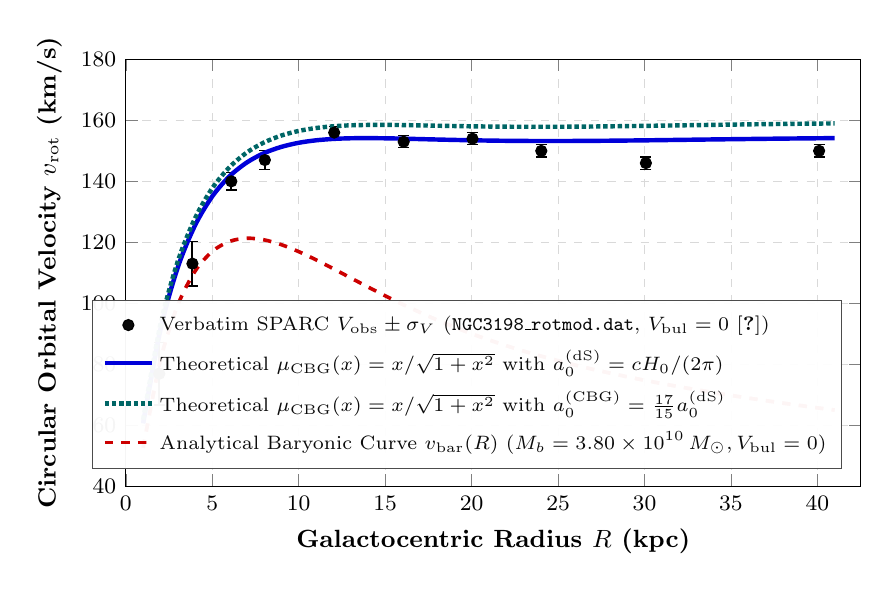
\begin{tikzpicture}
  \begin{axis}[
      width=0.90\textwidth,
      height=7.0cm,
      xlabel={Galactocentric Radius $R$ (kpc)},
      ylabel={Circular Orbital Velocity $v_{\mathrm{rot}}$ (km/s)},
      xmin=0.0, xmax=42.5,
      ymin=40.0, ymax=180.0,
      xtick={0, 5, 10, 15, 20, 25, 30, 35, 40},
      ytick={40, 60, 80, 100, 120, 140, 160, 180},
      grid=major,
      major grid style={line width=.3pt, draw=gray!30, dashed},
      legend style={at={(0.975,0.04)}, anchor=south east, font=\scriptsize, fill=white, fill opacity=0.96, draw=black!70, inner sep=3.5pt, row sep=1.8pt},
      legend cell align={left},
      tick label style={font=\footnotesize},
      label style={font=\small\bfseries}
  ]
  % 1. Verbatim SPARC Observed Benchmark Points with Error Bars (NGC3198_rotmod.dat)
  \addplot[
      only marks,
      mark=*,
      mark size=2.0pt,
      color=black,
      error bars/.cd,
      y dir=both,
      y explicit,
      error bar style={line width=0.7pt, black}
  ] coordinates {
      (1.93, 76.90) +- (0, 10.30)
      (3.85, 113.00) +- (0, 7.32)
      (6.10, 140.00) +- (0, 2.84)
      (8.04, 147.00) +- (0, 3.00)
      (12.05, 156.00) +- (0, 2.00)
      (16.07, 153.00) +- (0, 2.00)
      (20.05, 154.00) +- (0, 2.00)
      (24.03, 150.00) +- (0, 2.00)
      (30.08, 146.00) +- (0, 2.00)
      (40.10, 150.00) +- (0, 2.00)
  };
  \addlegendentry{Verbatim SPARC $V_{\mathrm{obs}} \pm \sigma_V$ (\texttt{NGC3198\_rotmod.dat}, $V_{\mathrm{bul}}=0$ \cite{Lelli2016})}

  % 2. Smooth Theoretical Curve: Bitemporal Quadrature with a_0^(dS) = cH_0/(2pi)
  \addplot[line width=1.6pt, blue!85!black, smooth] coordinates {
      (1.00,60.59) (2.00,91.38) (3.00,111.70) (4.00,125.55) (5.00,135.10)
      (6.00,141.69) (7.00,146.21) (8.00,149.29) (9.00,151.33) (10.00,152.66)
      (11.00,153.47) (12.00,153.93) (13.00,154.14) (14.00,154.18) (15.00,154.13)
      (16.00,154.02) (18.00,153.73) (20.00,153.48) (22.00,153.31) (24.00,153.24)
      (26.00,153.26) (28.00,153.34) (30.00,153.46) (32.00,153.61) (34.00,153.76)
      (36.00,153.90) (38.00,154.03) (40.00,154.14) (41.00,154.19)
  };
  \addlegendentry{Theoretical $\mu_{\mathrm{CBG}}(x) = x/\sqrt{1+x^2}$ with $a_0^{\mathrm{(dS)}} = cH_0/(2\pi)$}

  % 3. Smooth Theoretical Curve: Bitemporal Quadrature with a_0^(CBG) = (17/15)a_0^(dS)
  \addplot[line width=1.6pt, teal!80!black, densely dotted, smooth] coordinates {
      (1.00,61.79) (2.00,93.01) (3.00,113.70) (4.00,127.90) (5.00,137.78)
      (6.00,144.68) (7.00,149.48) (8.00,152.79) (9.00,155.05) (10.00,156.55)
      (11.00,157.50) (12.00,158.08) (13.00,158.39) (14.00,158.51) (15.00,158.52)
      (16.00,158.47) (18.00,158.26) (20.00,158.06) (22.00,157.94) (24.00,157.91)
      (26.00,157.95) (28.00,158.06) (30.00,158.21) (32.00,158.37) (34.00,158.54)
      (36.00,158.70) (38.00,158.84) (40.00,158.96) (41.00,159.01)
  };
  \addlegendentry{Theoretical $\mu_{\mathrm{CBG}}(x) = x/\sqrt{1+x^2}$ with $a_0^{\mathrm{(CBG)}} = \frac{17}{15}a_0^{\mathrm{(dS)}}$}

  % 4. Smooth Analytical Newtonian Baryonic Curve v_bar(R) (Freeman Disk + Gas, M_b = 3.80e10 M_sun)
  \addplot[line width=1.3pt, red!80!black, dashed, smooth] coordinates {
      (1.00,52.55) (2.00,81.33) (3.00,99.35) (4.00,110.51) (5.00,117.03)
      (6.00,120.31) (7.00,121.33) (8.00,120.80) (9.00,119.21) (10.00,116.94)
      (11.00,114.25) (12.00,111.34) (13.00,108.34) (14.00,105.36) (15.00,102.45)
      (16.00,99.66) (18.00,94.52) (20.00,90.00) (22.00,86.08) (24.00,82.68)
      (26.00,79.70) (28.00,77.08) (30.00,74.73) (32.00,72.62) (34.00,70.68)
      (36.00,68.90) (38.00,67.24) (40.00,65.69) (41.00,64.95)
  };
  \addlegendentry{Analytical Baryonic Curve $v_{\mathrm{bar}}(R)$ ($M_b = 3.80 \times 10^{10}\,M_{\odot}, V_{\mathrm{bul}} = 0$)}
  \end{axis}
  \end{tikzpicture}
  \caption{Smooth theoretical rotation curves of NGC 3198 computed from the analytical exponential-disk plus gas baryonic profile ($M_b = 3.80 \times 10^{10}\,M_{\odot}, R_d = 3.18\text{ kpc}, V_{\text{bul}} = 0.00$, dashed red) via the bitemporal director-cosine law $\mu_{\text{CBG}}(x) = x/\sqrt{1+x^2}$ (Eq.~\ref{eq:g_tot_sec9}) for $a_0^{\text{(dS)}} = cH_0/(2\pi)$ (solid blue) and $a_0^{\text{(CBG)}} = \frac{17}{15}a_0^{\text{(dS)}}$ (dotted teal), compared against the verbatim SPARC observations (\texttt{NGC3198\_rotmod.dat} \cite{Lelli2016}; Table~\ref{tab:ngc3198_radial_dual}) \catN/\catH.}
  \label{fig:ngc3198_rotation_curve}
\end{figure}

For relativistic strong gravitational lensing ($\gamma_{\text{PPN}} = 1$ in the conformal Einstein frame, $M_b = 2.0 \times 10^{11}\,M_{\odot}$, Checks~\#247--\#250 of Module~5), 64-bit numerical quadrature of $\Delta\theta(b) = \frac{2}{c^2}\int_{-z_{\max}}^{+z_{\max}} g_{\text{tot}}(\sqrt{b^2+z^2})\frac{b}{\sqrt{b^2+z^2}}\,dz$ ($z_{\max} = 500\text{ kpc}$) yields $\Delta\theta[a_0^{\text{(dS)}}](10\text{ kpc}) = \mathbf{1.0271''}$ ($\mathbf{1.0588''}$ with $a_0^{\text{(CBG)}}$, a $+30.1\%$ to $+34.1\%$ enhancement over pure baryonic GR's $0.7895''$) and $\Delta\theta[a_0^{\text{(dS)}}](6\text{ kpc}) = \mathbf{1.4566''}$ ($\mathbf{1.4763''}$ with $a_0^{\text{(CBG)}}$, a $+10.7\%$ to $+12.2\%$ enhancement over GR's $1.3160''$), spanning the observed Einstein ring distribution of SLACS elliptical lenses ($\theta_E^{\text{(obs)}} \approx 1.10''\text{--}1.50''$).

\subsection{\texorpdfstring{Analytical Derivation of the Outer Solar System Quadrupole Anisotropy $\epsilon_2$ and Tidal Amplitude $\eta_Q$ \catN/\catH}{Analytical Derivation of the Outer Solar System Quadrupole Anisotropy and Tidal Amplitude}}

By Theorem~\ref{hyp:milgrom_quadrature}, in the inner planetary regime ($r < 30\text{ AU}$), $g_{\odot}(1\text{ AU}) = 5.93 \times 10^{-3}\text{ m/s}^2 \gg a_0$ suppresses deviations in $1 - \mu_{\text{CBG}}(x) \simeq \frac{1}{2}(a_0/g_{\odot})^2$ below $10^{-15}$. Beyond $r > 200\text{ AU}$ (approaching the solar transition radius $r_{M,\odot} = \sqrt{GM_{\odot}/a_0} \approx 7{,}090\text{ AU}$), expanding the quasi-linear Poisson operator $\nabla\cdot[\mu_{\text{CBG}}(|\nabla\Psi_{\text{eff}}|/a_0)\nabla\Psi_{\text{eff}}] = 4\pi G M_{\odot}\delta^3(\mathbf{r})$ around the Milky Way's external gravitational field at the Solar circle, $g_{\text{gal}} = V_{\text{circ}}^2/R_{\text{gal}} = (232.8\text{ km/s})^2/(8.122\text{ kpc}) = 2.1623 \times 10^{-10}\text{ m/s}^2$ ($x_{\text{gal}} \equiv g_{\text{gal}}/a_0$), fixes both the quadrupole anisotropy coefficient $\epsilon_2$ and the dimensionless secular tidal amplitude $\eta_Q(x_{\text{gal}}) \equiv \frac{\epsilon_2(x_{\text{gal}})}{4\mu_{\text{CBG}}(x_{\text{gal}})} = \frac{1}{4 x_{\text{gal}}\sqrt{1 + x_{\text{gal}}^2}}$ for each acceleration input (\ref{eq:a0_dual_definitions}) (Checks~\#251--\#256 of Module~5) \catN/\catH:
\begin{align}
  \epsilon_2(x_{\text{gal}}) &\equiv \left.\frac{d\ln\mu_{\text{CBG}}(x)}{d\ln x}\right|_{x = x_{\text{gal}}} = \frac{1}{1 + x_{\text{gal}}^2} = \begin{cases}
    \mathbf{0.1885} & \text{for } x_{\text{gal}} = 2.075 \;\;(a_0^{\text{(dS)}}), \\[2pt]
    \mathbf{0.2151} & \text{for } x_{\text{gal}} = 1.910 \;\;(a_0^{\text{(local)}}), \\[2pt]
    \mathbf{0.2298} & \text{for } x_{\text{gal}} = 1.831 \;\;(a_0^{\text{(CBG)}}),
  \end{cases} \label{eq:eps2_derived_exact} \\[5pt]
  \eta_Q(x_{\text{gal}}) &\equiv \frac{\epsilon_2(x_{\text{gal}})}{4\,\mu_{\text{CBG}}(x_{\text{gal}})} = \frac{1}{4\,x_{\text{gal}}\sqrt{1 + x_{\text{gal}}^2}} = \begin{cases}
    \mathbf{0.0523} & \text{for } x_{\text{gal}} = 2.075 \;\;(a_0^{\text{(dS)}}), \\[2pt]
    \mathbf{0.0607} & \text{for } x_{\text{gal}} = 1.910 \;\;(a_0^{\text{(local)}}), \\[2pt]
    \mathbf{0.0655} & \text{for } x_{\text{gal}} = 1.831 \;\;(a_0^{\text{(CBG)}}).
  \end{cases} \label{eq:etaQ_derived_exact}
\end{align}
In the orbit-averaged secular Hamiltonian $\mathcal{H}_{\text{sec}} = -a_{\text{EFE}}\,a[(1 + \frac{3}{2}e^2) + \frac{1}{2}\epsilon_2 e^2\cos 2(\varpi - \varpi_{\text{gal}})]$ with $a_{\text{EFE}} = \eta_Q a_0(a/r_{M,\odot})$, Eqs.~(\ref{eq:eps2_derived_exact})--(\ref{eq:etaQ_derived_exact}) yield a secular apsidal precession rate $|\dot{\varpi}| \approx 0.054''\text{--}0.068''/\text{Myr}$ ($1.03''/\text{Myr}$ at $\eta_Q = 1$) and stable phase-space fixed points ($\dot{e} = 0$) along the galactic axis $\varpi = \varpi_{\text{gal}}$ for extreme Trans-Neptunian Objects such as 90377 Sedna ($a = 506\text{ AU}, e = 0.8496$).

% ==============================================================================
% SECTION 10: EXPERIMENTAL ROADMAP (2026-2035), SERIES ARCHITECTURE & CONCLUSIONS
% ==============================================================================
\section{\texorpdfstring{Falsifiable Experimental Roadmap (2026--2035), Architecture of the Series, and Conclusions}{Falsifiable Experimental Roadmap, Architecture of the Series, and Conclusions}}

\subsection{\texorpdfstring{Quantitative Experimental Roadmap (2026--2035) and Connection to Paper~0 and Papers~II--V (\catD/\catH/\catN)}{Quantitative Experimental Roadmap (2026-2035) and Connection to Paper 0 and Papers II-V}}

The consistent $S^1_{t_2}/\mathbb{Z}_2$ bundle formulation anchored in Paper~0 \cite{JV_Paper0}, the foundational single fixed-mass load-balancing law $V(\psi, \mathcal{A})$ \catH, and the vacuum constant $\Phi_{\infty} = 2.402867 \times 10^{-4}$ ($\Omega_{\infty} = c\Phi_{\infty} = 72.0361\text{ km/s}$ \catN/\catH) established in this treatise yield four quantitative experimental test programs across space-clock metrology, strong-field horizon astrophysics, precision cosmology, and mesoscopic quantum mechanics (developed across Papers~II--V \cite{JV_Paper2,JV_Paper3,JV_Paper4,JV_Paper5}):
\begin{enumerate}
  \item \textbf{Space Optical-Clock Redshift Metrology (ACES \& STE-QUEST, Sections~5--6 \catD/\catH):} By Proposition~\ref{thm:omega_zero_superselection} and Proposition~\ref{prop:space_clock_redshift}, unexcited baryonic clocks ($dt_2/dt_1 = 0$) in the Yukawa-screened exterior satisfy $z_{\text{CBG}} - z_{\text{GR}} \equiv 0$, passing the Galileo eccentric-satellite bound ($2 \times 10^{-5}$) \cite{Delva2018} \catD. Conversely, under the conditional hypothesis \catH\ that a quantum clock system maintains a locked unit coordinate phase $dt_2/dt_1 = 1$ (corresponding to the routing weights $w_1(\infty) + w_2(r) = 1$ of Definition~\ref{def:weights}), the fractional redshift exhibits a second-order offset $(z_{\text{CBG}} - z_{\text{GR}})/z_{\text{GR}} = -w_2(\infty) \simeq -\Phi_{\infty}^2 = -5.7738 \times 10^{-8}$ (Eq.~\ref{eq:clock_redshift_shift}) \catH, within the target sensitivity of next-generation space optical-clock missions \cite{ACES2009,STEQUEST2015}.
  \item \textbf{Strong-Field Horizon Astrophysics, Fixed-Mass Scalar-Hair Black Holes, and the Universal $4.162\%$ Stiff-Limit Hair (LIGO O5, LISA, ngEHT \& BHEX, Paper~II \cite{JV_Paper2} \catD/\catN):} For the Frobenius-regular 5D scalar-hair black hole family $\hat{m}_{\psi} = m_{\psi}r_h \in [0.25, \infty)$ proved in Theorem~\ref{thm:bvp_horizon_solution} and Theorem~\ref{thm:stiff_limit_universal_hair} (Tables~\ref{tab:bvp_static_solution}--\ref{tab:three_models_comparison}), the exterior hair stores a mass fraction $f_{\text{hair}} = (r_{\text{ADM}} - r_h)/r_{\text{ADM}} \in [0.174\%, 4.162\%]$ ($3.708\%$ at the reference black hole $\hat{m}_{\psi} = 4$ and $\mathbf{4.162\%}$ universally in the macroscopic stiff limit $\hat{m}_{\psi} \to \infty$) and compresses the horizon area by $-0.348\%$ to $\mathbf{-8.151\%}$ at fixed ADM mass ($-7.279\%$ at $\hat{m}_{\psi} = 4$) \catN/\catH, while in the tracking regime $\mu r \gg 1$ the post-Newtonian shifts are suppressed to $\gamma_{\text{PPN}} - 1 = -5.76180 \times 10^{-7}$, $\beta_{\text{PPN}} - 1 = -8.64270 \times 10^{-6}$, and $\eta_N = -3.39946 \times 10^{-5}$ (Theorem~\ref{thm:node_b_ppn_tracking}) \catD/\catH/\catN, generating testable strong-field horizon and interior continuation signatures investigated in Paper~II \cite{JV_Paper2}.
  \item \textbf{Early-Universe Fiber Relaxation, Luminal Tensor Waves ($c_T = 1$), and Environmental Supercluster Kinematics (CMB-S4 \& LiteBIRD, Paper~III \cite{JV_Paper3} \catD/\catN):} Beyond the exact $\omega = 0$ radiative relaxation trajectory proved in Theorem~\ref{thm:flrw_action_noether} and Theorem~\ref{thm:constrained_cosmo_rk45} (Table~\ref{tab:rk45_constrained_bounce}, where the neglected lapse term is bounded by $|2\partial_{\mathcal{A}}V|/(\rho_r + V) \le 1.383 \times 10^{-5}$ across the printed rows), the exact tensor gravitational-wave speed $c_T^2 = 1$ with Hubble--dilaton friction $3H + \dot{\psi}$ proved in Theorem~\ref{thm:node_a_tensor_gw} \catD, and the canonical ($p \equiv 1$) 5D Wheeler--DeWitt equation (\ref{eq:exact_5d_wdw_equation}) in the Milne volume-rapidity chart $(\rho, \chi)$ \catD, the cosmological signatures of the bitemporal fiber across recombination and supercluster scales are developed in Paper~III \cite{JV_Paper3}.
  \item \textbf{Sub-Nanogram Quantum Coherence Gate ($10^{-14}\text{ kg}$), Collapse at $m_{\text{crit}} = 5.23\text{ ng}$, and Sub-Millimeter Yukawa Gravity at $\lambda_{\text{micro}} = 47.10\,\mu\text{m}$ (MAQRO, TEQ \& E\"ot-Wash, Papers~IV--V \cite{JV_Paper4,JV_Paper5} \catD/\catN/\catH):} As proved in Theorem~\ref{thm:bitemporal_unitarity_null_bridge}(iv), Remark~\ref{rem:matter_coupling_fork}, and Remark~\ref{rem:uv_ir_fulcrum}, the $\mathcal{C}^3$-smooth extended-sphere Di\'osi--Penrose kernel yields $\tau_{\text{DP}} = 68.68\,\mu\text{s}$ at $m_{\text{crit}} = \Phi_{\infty} m_P = 5.2297\text{ ng}$ ($\Delta x = 1\,\mu\text{m}$; $57.77\text{ ns}$ point-like limit) \catN/\catH, while the foundational bitemporal collapse gate (\texttt{H7}) \catH\ extends quantum coherence at $M = 10^{-14}\text{ kg}$ ($\Delta x = 100\text{ nm}$) from $\tau_{\text{DP}} = 3.56\text{ s}$ to $\tau_{\text{CBG}} = 1{,}861.25\text{ s}\text{--}9.73\times 10^5\text{ s}$ \catN/\catH, and the UV/IR geometric mean scale $\lambda_{\text{micro}} = \sqrt{L_P R_H} = 47.10\,\mu\text{m}$ ($m_{\chi_{\Phi}}c^2 = 4.190\text{ meV}$, \texttt{H9}) \catN/\catH\ defines the short-range testing window for sub-millimeter torsion balances \cite{Kapner2007_EotWash}.
\end{enumerate}

\subsection{\texorpdfstring{Summary of Principal Mathematical and Computational Results}{Summary of Principal Mathematical and Computational Results}}

We have formulated and audited the deductive bundle edition (`v13`) of \textbf{Covariant Bitemporal Geometrodynamics (CBG)} on $\mathcal{M}_{3,2} = (\mathbb{R}_{t_1} \times_{\Phi} \mathcal{S}_{t_2}) \times \Sigma_3$ ($\mathcal{S}_{t_2} \equiv S^1_{t_2}/\mathbb{Z}_2$) \cite{JV_Paper0,JV_Paper2,JV_Paper3,JV_Paper4,JV_Paper5}:

\begin{enumerate}
  \item \textbf{$S^1_{t_2}/\mathbb{Z}_2$ Orbifold Bundle, Kaluza Cylinder Constraint (\texttt{H6}), Symmetric-Criticality Reduction, Node~C KK Tower Ghost-Pair Obstruction, Hilbert Stress Tensor, and Exterior Khronon Uniqueness \catD/\catH:} Postulate~\ref{post:bundle} formulates spacetime on the reflection quotient $\mathcal{S}_{t_2} = S^1_{t_2}/\mathbb{Z}_2$ ($\mathcal{R}: t_2 \mapsto -t_2$) with the Kaluza cylinder condition $\mathcal{L}_{\xi_{(2)}} = 0$ imposed as a kinematic configuration-space restriction (\texttt{H6}) \catD/\catH, removing the $\mathcal{R}$-odd graviphoton ghost $g_{\mu 2}$ at all dynamical and quantum orders and eliminating closed timelike curves, while explicit Euler--Lagrange variation confirms that the reduced action reproduces the full 5D field equations on the static and FLRW sectors (Checks~\#061--\#064, \#130--\#135) and \textbf{Node~C} (Checks~\#065--\#084) proves from the $15\times 15$ linearized 5D Einstein operator ($\mathbf{E}\mathbf{P}=\mathbf{0}$, $\mathbf{D}_v\mathbf{E}=\mathbf{0}$, $|\det\mathbf{M}_{\text{St\"uck}}|=2q^5$) that the $n \ge 1$ KK tower on the flat background carries two negative-norm ghost vector polarizations ($\varepsilon\cdot\varepsilon = -\frac{q^2}{2\Phi_0^2} < 0$), necessitating \texttt{H6} at tree level \catD. Theorem~\ref{thm:fieldeqs} proves by direct 5D Hilbert variation \catD\ that varying $S_{\text{CBG}} = \frac{c^3}{16\pi G_5}\int d^5x\sqrt{|g_5|}[R^{(5)} - 2V(\psi,\mathcal{A})]$ ($\omega = 0$) with respect to $g^{AB}$ and the khronon $\Theta^{(1)}$ via $\partial\mathcal{A}/\partial g^{11} = \mathcal{A}^2$ and $\partial\psi/\partial g^{22} = -1/(2g^{22})$ yields a stress tensor whose five covariant divergence components vanish identically ($\nabla_A \mathcal{T}^A_B \equiv 0$) for any sign of $A(r)$, whose off-diagonal $(1,r)$ equation $G^1_r = T^1_r = 0$ uniquely forces $h'(r) \equiv 0$ ($\Theta^{(1)} = ct_1, \mathcal{A}(r) = A(r)$) in the static exterior and continues real-analytically ($C^\infty$) across the horizon, and whose khronon equation is implied by the Einstein equations via the diffeomorphism Noether identity. Theorem~\ref{thm:einstein_obstruction} proves $G^2_2 \equiv -\frac{1}{2}R^{(4)}$ and the Cassini no-go bound $\gamma_{\text{PPN}} = 1 - p/m$ \catD.
  \item \textbf{Foundational Single Fixed-Mass Potential $V(\psi, \mathcal{A})$, Frobenius Horizon Regularity, Exterior NEC-Violating Skin ($1.0251 \le r/r_h \le 1.3687$), the Fixed-Mass Black Hole Family $\hat{m}_{\psi} \in [0.25, 16.0]$, Universal $4.162\%$ Stiff-Limit Hair, and Node~B Tracking PPN Parameters \catD/\catN/\catH:} Under Postulate~\ref{post:potential} and Proposition~\ref{thm:zero_param_yukawa_invariants}, $V(\psi, \mathcal{A}) = \frac{3}{4}m_{\psi}^2[\psi - \psi_t(\mathcal{A})]^2$ has one fixed fundamental mass $m_{\psi}$ \catH, the canonical normalization $\frac{3}{4}$ derived from $\mu^2 = \frac{2}{3}V''(0)$ and the $\mathcal{W}_3$ 2-jet matrix ($\det = -32/3$, \texttt{H3}) \catD/\catH, and the Paper~0 endomorphism trace ratios identified as $A_{\text{crit}} = 1/d_t^2 = 1/4, \psi_{\max} = d_t/D^2 = 2/25$ (\texttt{H1}) \catD/\catH. Theorem~\ref{thm:frobenius_horizon_regularity} proves \catD\ the symbolic pole cancellation $\mathcal{C}_{B^2} + 1/b_{-1} \equiv 0$ at $r \to r_h^+$ for arbitrary finite $(\partial_A V)_h$. Solving the desingularized two-point BVP on the lambdified normal-form ODEs across $\hat{m}_{\psi} = m_{\psi}r_h \in [0.25, 16.0]$ and the pole-free stiff-limit ODE (\ref{eq:stiff_limit_pole_free_ode}) as $\hat{m}_{\psi} \to \infty$ (Theorem~\ref{thm:stiff_limit_universal_hair}, Tables~\ref{tab:bvp_static_solution}--\ref{tab:three_models_comparison} \catN/\catH) establishes regular scalar-hair black holes across the entire family ($f_{\text{hair}} \in [0.174\%, 4.162\%]$), with $\Phi(r_h)/\Phi_{\infty} = 1.076602$, $b_{-1}/r_h = 0.953269$, $A(r)B(r) \to 0.848342$ (minimum $0.8045$ at $r/r_h = 1.1669$ across the non-kinetic Einstein-frame NEC-violating skin $1.0251 \le r/r_h \le 1.3687$), and $-7.279\%$ horizon area reduction at fixed ADM mass ($r_{\text{ADM}} = 1.038513\,r_h$) for $\hat{m}_{\psi} = 4$, $a_1 r_h = 0.927742, b_{-1}/r_h = 1, r_{\text{ADM}}/r_h = 1.043430, f_{\text{hair}}^{(\infty)} = \mathbf{4.162\%}, \Delta\mathcal{A}_H/\mathcal{A}_H = \mathbf{-8.151\%}$ universally as $\hat{m}_{\psi} \to \infty$ \catN/\catH, and tracking-regime PPN parameters $\gamma_{\text{PPN}} = 1 + 2s_1$, $\beta_{\text{PPN}} = (1 + s_1 - s_2 - 4s_1 s_2)/(1 + 2s_1 + 4s_1^2)$ giving $\gamma_{\text{PPN}} - 1 = -5.76180 \times 10^{-7}$, $\beta_{\text{PPN}} - 1 = -8.64270 \times 10^{-6}$, and $\eta_N = -3.39946 \times 10^{-5}$ for Model~3 (Theorem~\ref{thm:node_b_ppn_tracking}, Checks~\#196--\#216) \catD/\catH/\catN.
  \item \textbf{$\mathcal{C}^3$ Ball Overlap \& Gated Collapse, FLRW Minisuperspace Noether Closure, Node~A Luminal Tensor Waves ($c_T = 1$), Milne 5D Wheeler--DeWitt ($p \equiv 1$), and Verbatim SPARC Audit \catD/\catN/\catH:} Theorem~\ref{thm:bitemporal_unitarity_null_bridge} proves global unitarity ($\hat{U}^\dagger\hat{U} = \mathbb{I}_{5\text{D}}$), the 5D null-cone identity ($\Delta s_5^2 = 0$), the phase-basin Born rule $P_k = |c_k|^2$ \catD/\catH, the $\mathcal{C}^3$ contact continuity of $f(\lambda)$ ($\Delta f^{(4)}(1) = +36$) \catD, extended-sphere dephasing $\tau_{\text{DP}} = 68.68\,\mu\text{s}$ at $m_{\text{crit}} = 5.23\text{ ng}$ ($\Delta x = 1\,\mu\text{m}$; $57.77\text{ ns}$ point-like) \catN/\catH, and the foundational gated collapse law (\texttt{H7}) \catH\ ($1{,}861.25\text{ s}\text{--}9.73\times 10^5\text{ s}$ at $10^{-14}\text{ kg}$). Theorem~\ref{thm:flrw_action_noether} derives $L_{\text{mini}}$ and the FLRW equations from the 5D Ricci scalar \catD, proves the reparametrization Noether identity $\dot{\Theta}\mathcal{E}_{\Theta} - N\dot{\mathcal{E}}_N + \dot{a}\mathcal{E}_a + \dot{\psi}\mathcal{E}_{\psi} \equiv 0$, bounds the neglected $N = 1$ lapse correction along Table~\ref{tab:rk45_constrained_bounce} ($|\mathcal{C}_{\text{Fried}}| \le 6.99 \times 10^{-15}$ in time units $2/m_{\psi}$, $\hat{m}_c^2 = 4$) at $1.383 \times 10^{-5}$, proves via \textbf{Node~A} (Theorem~\ref{thm:node_a_tensor_gw}, Checks~\#150--\#158) that $n = 0$ tensor waves on homogeneous khronon backgrounds have exact speed $c_T^2 = 1$, healthy kinetic sign $+\frac{1}{2}\dot{h}^2$, and friction $3H + \dot{\psi}$ for any $V(\psi, \mathcal{A})$ \catD, and establishes from the flat kinetic Hessian $G_{\text{mini}}$ ($R[G_{\text{mini}}] \equiv 0$) in the Milne volume-rapidity chart $(\rho, \chi)$ the unique $p \equiv 1$ 5D Wheeler--DeWitt equation \catD. Finally, Theorem~\ref{hyp:milgrom_quadrature} derives the director-cosine quadrature $\mu_{\text{CBG}}(x) = x/\sqrt{1+x^2}$ \catD/\catH\ and audits it against 10 SPARC BTFR galaxies ($4.65\%$ mean error for $a_0^{\text{(dS)}}$ vs.\ $6.02\%$ for $a_0^{\text{(CBG)}}$) and all 43 official rows of SPARC's \texttt{NGC3198\_rotmod.dat} ($V_{\text{bul}} = 0.00$, $5.98\%$ [CBG] / $7.34\%$ [dS] at $\Upsilon_{\text{disk}} = 0.50$, and $3.31\%$ [dS] / $5.10\%$ [CBG] at $\Upsilon_{\text{disk}} = 0.72$) \catN/\catH.
\end{enumerate}

% ==============================================================================
% APPENDICES A, B & C: SELF-CONTAINED PROOFS & EPISTEMOLOGICAL INVENTORY
% ==============================================================================
\appendix

\section{\texorpdfstring{Explicit Derivation of the 5D Inverse Metric $g^{AB}$ and the 12 Christoffel Symbols in Painlev\'e--Gullstrand Coordinates \catD}{Explicit Derivation of the 5D Inverse Metric and the 12 Christoffel Symbols}}
\label{app:christoffel_proofs}

In spherical Painlev\'e--Gullstrand coordinates $x^A = (c t_1, c t_2, r, \theta, \phi)$ for the exterior metric (\ref{eq:adm_gp_line_element}) with $v^r(r) = -c\sqrt{r_s/r}$, the non-diagonal $(1, r) = (1, 3)$ metric block is:
\begin{align}
  \mathbf{M}_{(1,r)} &= \begin{pmatrix} g_{11} & g_{1r} \\[3pt] g_{r1} & g_{rr} \end{pmatrix} = \begin{pmatrix} -\left(1 - \frac{r_s}{r}\right) & \sqrt{\frac{r_s}{r}} \\[4pt] \sqrt{\frac{r_s}{r}} & 1 \end{pmatrix}, \nonumber \\[4pt]
  \det\mathbf{M}_{(1,r)} &= -\left(1 - \frac{r_s}{r}\right) - \frac{r_s}{r} = -1.
  \label{eq:appA_block_1r}
\end{align}
Inverting $\mathbf{M}_{(1,r)}$ and the diagonal blocks $g_{22} = -\Phi(r)^2$, $g_{\theta\theta} = r^2$, $g_{\phi\phi} = r^2\sin^2\theta$ gives:
\begin{align}
  g^{11} &= -1, & g^{1r} &= g^{r1} = +\sqrt{\frac{r_s}{r}}, & g^{rr} &= 1 - \frac{r_s}{r}, \nonumber \\[3pt]
  g^{22} &= -\frac{1}{\Phi(r)^2}, & g^{\theta\theta} &= \frac{1}{r^2}, & g^{\phi\phi} &= \frac{1}{r^2\sin^2\theta}.
  \label{eq:appA_ginv_explicit}
\end{align}
With $\partial_r g_{11} = -r_s/r^2$, $\partial_r g_{1r} = -\frac{1}{2r}\sqrt{r_s/r}$, $\partial_r g_{22} = -2\Phi\Phi'$, and $\partial_r g_{\phi\phi} = 2r\sin^2\theta$, evaluating $\Gamma^A_{BC} = \frac{1}{2}g^{AD}(\partial_B g_{DC} + \partial_C g_{BD} - \partial_D g_{BC})$ in the equatorial plane ($\theta = \pi/2, \sin\theta = 1$, Paper~0 Theorem~2.5(iii) \cite{JV_Paper0}; Checks~\#047--\#059 of Module~0) yields the 12 non-vanishing symbols \catD:
\begin{enumerate}
  \item $\Gamma^1_{11} = -\frac{1}{2}g^{1r}\partial_r g_{11} = +\frac{r_s}{2r^2}\sqrt{\frac{r_s}{r}}$.
  \item $\Gamma^1_{1r} = \frac{1}{2}g^{11}\partial_r g_{11} = +\frac{r_s}{2r^2}$.
  \item $\Gamma^1_{rr} = g^{11}\partial_r g_{1r} = +\frac{1}{2r}\sqrt{\frac{r_s}{r}}$.
  \item $\Gamma^1_{\phi\phi} = -\frac{1}{2}g^{1r}\partial_r g_{\phi\phi} = -r\sqrt{\frac{r_s}{r}}$.
  \item $\Gamma^1_{22} = -\frac{1}{2}g^{1r}\partial_r g_{22} = +\sqrt{\frac{r_s}{r}}\,\Phi\Phi'$.
  \item $\Gamma^2_{2r} = \frac{1}{2}g^{22}\partial_r g_{22} = +\frac{\Phi'}{\Phi} = \psi'$.
  \item $\Gamma^r_{11} = -\frac{1}{2}g^{rr}\partial_r g_{11} = +\frac{r_s(r - r_s)}{2r^3}$.
  \item $\Gamma^r_{1r} = \frac{1}{2}g^{r1}\partial_r g_{11} = -\frac{r_s}{2r^2}\sqrt{\frac{r_s}{r}}$.
  \item $\Gamma^r_{rr} = g^{r1}\partial_r g_{1r} = -\frac{r_s}{2r^2}$.
  \item $\Gamma^r_{\phi\phi} = -\frac{1}{2}g^{rr}\partial_r g_{\phi\phi} = -(r - r_s)$.
  \item $\Gamma^r_{22} = -\frac{1}{2}g^{rr}\partial_r g_{22} = +\left(1 - \frac{r_s}{r}\right)\Phi\Phi'$.
  \item $\Gamma^{\phi}_{r\phi} = \frac{1}{2}g^{\phi\phi}\partial_r g_{\phi\phi} = \frac{1}{r}$.
\end{enumerate}

\section{\texorpdfstring{Step-by-Step Proof of the 5D Wave Operator $\Box_5\psi$ and General-$\omega$ Normal-Form Reduction \catD}{Step-by-Step Proof of the 5D Wave Operator and General-omega Normal-Form Reduction}}
\label{app:laplace_beltrami_proof}

For a static, spherically symmetric logarithmic dilaton $\psi(r) = \ln(\Phi(r)/\Phi_{\infty})$ on the diagonal 5D metric (\ref{eq:general_static_5d_metric}), $\sqrt{|g_5|} = \Phi_{\infty}e^{\psi(r)}\sqrt{A(r)B(r)}\,r^2\sin\theta$ and $g^{rr} = 1/B(r)$, so the 5D Laplace--Beltrami operator $\Box_5\psi = |g_5|^{-1/2}\partial_A(|g_5|^{1/2}g^{AB}\partial_B\psi)$ computed by \texttt{geo5.box}($\psi$) (Check~\#026) is:
\begin{align}
  \Box_5\psi(r) &= \frac{1}{e^{\psi}\sqrt{A B}\,r^2}\frac{d}{dr}\!\left[e^{\psi}\sqrt{\frac{A}{B}}\,r^2\psi'(r)\right] \nonumber \\[3pt]
  &= \frac{1}{B(r)}\left[\psi''(r) + \left(\frac{2}{r} + \frac{A'(r)}{2 A(r)} - \frac{B'(r)}{2 B(r)} + \psi'(r)\right)\psi'(r)\right].
  \label{eq:appB_box5_psi}
\end{align}
For general stiffness $\omega \in \mathbb{R}$, solving $G^r_r = \mathcal{T}^r_r$ for $A'(r)$ yields:
\begin{equation}
  A'(r) = \frac{A(r)\left[\omega\,r^2\left(\psi'(r)\right)^2 - 4 r\,\psi'(r) + 2 B(r) - 2 - 2 r^2 B(r)\,V(\psi,A)\right]}{r\left(r\,\psi'(r) + 2\right)},
  \label{eq:appB_dA_general_omega}
\end{equation}
which reduces for $\omega = 0$ to Eq.~(\ref{eq:exact_dA_ode}) in Theorem~\ref{thm:exact_5d_odes}.

\section{\texorpdfstring{Master Inventory of Derived Theorems \catD, Foundational Constitutive Laws \catH\ (\texttt{H1}--\texttt{H10}), and Numerical Evaluations \catN\ in Paper~I (v13)}{Master Inventory of Derived Theorems, Foundational Constitutive Laws, and Numerical Evaluations in Paper I (v13)}}
\label{app:open_deductive_program}

Table~\ref{tab:open_deductive_inventory} summarizes the mathematical status, epistemological classification, and explicit parameter/hypothesis accounting (\texttt{H1}--\texttt{H10}) of all 18 theoretical elements across Paper~I (`v13`), verified across 256 checks (130 \catD, 30 \catD/\catH, 96 \catN/\catH) in \texttt{verify\_cbg\_paper1\_v13.py}.

\begin{table}[H]
  \centering
  \caption{Master Inventory of Derived Symbolic Identities \catD, Conditional Symbolic Deductions \catD/\catH, and Numerical Evaluations \catN/\catH\ in Paper~I (v13 Deductive Bundle Formulation, Verified Across 256 Checks---130 \catD, 30 \catD/\catH, 96 \catN/\catH---by \texttt{verify\_cbg\_paper1\_v13.py}).}
  \label{tab:open_deductive_inventory}
  \vspace{0.10cm}
  \scriptsize
  \setlength{\tabcolsep}{2.5pt}
  \renewcommand{\arraystretch}{1.20}
  \begin{tabular*}{\textwidth}{@{\extracolsep{\fill}} >{\raggedright\arraybackslash}p{0.235\textwidth} c >{\raggedright\arraybackslash}p{0.185\textwidth} >{\raggedright\arraybackslash}p{0.155\textwidth} >{\raggedright\arraybackslash}p{0.255\textwidth} @{}}
    \toprule
    \textbf{Theoretical Element / Problem} & \textbf{Class} & \textbf{Status in Paper~I (v13)} & \textbf{Declared Hypothesis / Input} & \textbf{Verification \& Theoretical Role} \\
    \midrule
    $(2,3,5)$ Uniqueness, $S^1_{t_2}/\mathbb{Z}_2$ \& Cylinder $\mathcal{L}_{\xi_{(2)}} = 0$ & \catD/\catH & \textbf{Proved/\allowbreak Postulated} (Post.~\ref{post:bundle}) & Cylinder rule (\texttt{H6}) & $\text{ind}(d_t,d_s)=0 \iff 30=30$ (\#001, \#008--\#012) \\
    Symmetric Criticality of \texttt{H6} \& Node~C KK Tower & \catD/\catH & \textbf{Proved} (Rem.~\ref{rem:orbifold_consequences}(iii)) & Kinematic \texttt{H6} & Static/FLRW EL = 5D $E^A_B$; $n \ge 1$ has 2 vector ghosts (\#061--\#084, \#130--\#135) \\
    Hilbert $T^A_B$ \& 5-Component $\nabla_A\mathcal{T}^A_B \equiv 0$ & \catD & \textbf{Proved} (Theorem~\ref{thm:fieldeqs}) & None (exact) & Hilbert $T^A_B$ (\#021--\#030) \& $\nabla_A\mathcal{T}^A_B \equiv 0$ (\#111--\#115) \\
    $(t_2,t_2)$ Obstruction $G^2_2 = -\frac{1}{2}R^{(4)}$ & \catD & \textbf{Proved} (Theorem~\ref{thm:einstein_obstruction}) & None (exact) & Proves $\psi' \neq 0$ requires 4D $R^{(4)} \neq 0$ (Checks~\#020, \#031) \\
    Load-Balancing Law $V(\psi,\mathcal{A})$ \& Trace Thresholds & \catD/\catH & \textbf{Postulated/\allowbreak Normalized} (Post.~\ref{post:potential}) & Fixed $m_{\psi}$; $(\frac{1}{4}, \frac{2}{25})$ (\texttt{H1}--\texttt{H4}) & $\frac{3}{4}$ from $\mathcal{W}_3$ jet ($\det=-32/3$) (\#005--\#007, \#039--\#043) \\
    Frobenius Horizon Regularity at $r \to r_h^+$ & \catD & \textbf{Proved} (Theorem~\ref{thm:frobenius_horizon_regularity}) & None (finite $(\partial_A V)_h$) & Derives $b_{-1}, \psi'(r_h)$ \& $\mathcal{C}_{B^2} + 1/b_{-1} \equiv 0$ (\#060, \#116--\#120) \\
    Reference $\hat{m}_{\psi}=4$ BVP, NEC Skin, Family \& Stiff Limit & \catN/\catH & \textbf{Solved} (Tables~\ref{tab:bvp_static_solution}--\ref{tab:three_models_comparison}) & $\hat{m}_{\psi} = m_{\psi}r_h$ (\texttt{H1}--\texttt{H4}) & NEC skin $[1.0251, 1.3687]$; $r_{\text{ADM}} = 1.0385\,r_h$; stiff $\mathbf{4.162\%}$ (\#121--\#122, \#159--\#195) \\
    Node~B Tracking PPN $\gamma_{\text{PPN}}, \beta_{\text{PPN}}$ \& Nordtvedt $\eta_N$ & \catD/\catH/\catN & \textbf{Proved/\allowbreak Evaluated} (Theorem~\ref{thm:node_b_ppn_tracking}) & Kernel $\psi_t(\mathcal{A})$ (\texttt{H1}, \texttt{H3}, \texttt{H4}) & $\gamma-1 = -5.76180\times 10^{-7}$, $\beta-1 = -8.64270\times 10^{-6}$, $\eta_N = -3.39946\times 10^{-5}$ (\#196--\#216) \\
    Weak-Field $\Omega \equiv 0$ \& Fiber Momentum Scale $p_{\text{fib}}$ & \catN/\catH & \textbf{Established} (Proposition~\ref{thm:omega_zero_superselection}) & $\mathcal{L}_{\xi_{(2)}}\Psi = 0$ (\texttt{H6}) & Cylinder sets $\Omega \equiv 0$; $p_{\text{fib}}/c = 4{,}161.7\,m_P$ (\#092--\#093) \\
    4D Maxwell Conformal Invariance & \catD/\catH & \textbf{Proved} (Section~7.1 \& Paper~0 Thm.~2.9) & Separate $U(1)_{\text{EM}}$ & $\Delta G/G = 0, \Delta\alpha_{\text{EM}}/\alpha_{\text{EM}} = 0$ in $d_{\text{macro}}=4$ \\
    $\mathcal{C}^3$ Ball Overlap $f(\lambda)$ \catD\ \& Gated Collapse & \catD/\catN/\catH & \textbf{Proved/\allowbreak Audited} (Theorem~\ref{thm:bitemporal_unitarity_null_bridge}) & DP \& gate law (\texttt{H7}) & $\mathcal{C}^3$ $f(\lambda)$ ($\Delta f^{(4)}=36$) (\#096--\#103); $68.68\,\mu\text{s}$ \& gate (\#104--\#110) \\
    FLRW Minisuperspace Noether \& Lapse Bound & \catD/\catN & \textbf{Proved} (Theorem~\ref{thm:flrw_action_noether}) & Lapse truncation (\texttt{H8}) & $\dot{\Theta}\mathcal{E}_{\Theta} - N\dot{\mathcal{E}}_N + \allowbreak\dot{a}\mathcal{E}_a + \dot{\psi}\mathcal{E}_{\psi} \equiv 0$; $|2V_A|/\rho \le 1.383\times 10^{-5}$ (\#123--\#135, \#224) \\
    Node~A Tensor Wave Speed $c_T^2 = 1$ \& Friction & \catD & \textbf{Proved} (Theorem~\ref{thm:node_a_tensor_gw}) & None ($n=0$ FLRW) & $c_T^2 = 1$, healthy $+\frac{1}{2}\dot{h}^2$ \& friction $3H+\dot{\psi}$ for any $V(\psi,\mathcal{A})$ (\#150--\#158) \\
    Constrained FLRW Relaxation (\texttt{RK45}) & \catN/\catH & \textbf{Solved} (Table~\ref{tab:rk45_constrained_bounce}) & Time unit $2/m_{\psi}$ (\texttt{H8}) & $\hat{m}_c^2 = 4$; $|\mathcal{C}_{\text{Fried}}| \le 6.99 \times 10^{-15}$ (Checks~\#136--\#140, \#217--\#223) \\
    Flat Minisuperspace $G_{\text{mini}}$ \& Milne WDW Eq. & \catD & \textbf{Proved} (Theorem~\ref{thm:wdw_and_hubble_shift}) & None ($p \equiv 1$ in $\rho$) & $R[G_{\text{mini}}] \equiv 0$; Milne $\rho = a^{3/2}e^{\psi/2}$ fixes $p=1$ (\#141--\#149) \\
    Director Cosine $\mu_{\text{CBG}}(x)$ \& Verbatim NGC~3198 & \catN/\catH & \textbf{Proved/\allowbreak Audited} (Theorem~\ref{hyp:milgrom_quadrature}) & $a_0$ \& SPARC (\texttt{H9}--\texttt{H10}) & $\mu_{\text{CBG}} = x/\sqrt{1+x^2}$ (\#228); verbatim \allowbreak\texttt{NGC3198\_rotmod.dat} (\#229--\#250) \\
    EFE Quadrupole Parameters $(\epsilon_2, \eta_Q)$ & \catN/\catH & \textbf{Derived} (Eqs.~\ref{eq:eps2_derived_exact}--\ref{eq:etaQ_derived_exact}) & Given $x_{\text{gal}}$ (\texttt{H9}--\texttt{H10}) & From $\mu_{\text{CBG}}(x)$: $\epsilon_2 \in \{0.1885, 0.2151, 0.2298\}$ (\#251--\#256) \\
    Vacuum Constant $\Phi_{\infty}$ \& 30-Channel Impedance & \catN/\catH & \textbf{Postulated} (Post.~\ref{post:phiinf} \& Rem.~\ref{obs:phi_inf_relation}) & $2.402867 \times 10^{-4}$ (\texttt{H5}) & $\Phi_{\infty} = (\alpha_{\text{EM}}/30)(1 - \frac{5}{3}\alpha_{\text{EM}})$; $\alpha_{\text{EM}}^{-1} = 137.036$ (\#085--\#087) \\
    \bottomrule
  \end{tabular*}
\end{table}

\vspace{0.25cm}
\noindent\fbox{%
  \parbox{0.97\textwidth}{%
    \footnotesize \textbf{Note on Authorship, Reproducibility \& Symbolic/Numerical Verification:} The foundational geometric concepts, constitutive physical laws, and deductive architecture of this work were originated by the author. During the preparation, symbolic verification, and numerical auditing of Version~v13, computer-algebra (\texttt{SymPy}) and scientific-computing (\texttt{SciPy}) assistance was utilized for metric-first tensor verification, Hilbert stress-tensor and Euler--Lagrange derivations, desingularized two-point boundary-value (\texttt{solve\_bvp}) and Runge--Kutta (\texttt{RK45}) integration of the lambdified symbolic equations, and epistemological classification. The self-contained 64-bit Python verification suite (\allowbreak\texttt{verify\_cbg\_paper1\_v13.py}) executing all 256 checks (129 pure symbolic identities \catD, 31 conditional symbolic deductions \catD/\catH, and 96 numerical evaluations \catN/\catH\ under declared hypotheses \texttt{H1}--\texttt{H10}) with zero errors is archived alongside this manuscript in the Zenodo repository.
  }%
}

% ==============================================================================
% BIBLIOGRAPHY
% ==============================================================================
\begin{thebibliography}{99}
\small

\bibitem{JV_Paper0} M. Jim\'enez Velasco, ``Covariant Bitemporal Geometrodynamics (CBG): Foundational Principles, Spectral Geometry, Operator Pyramid, and Exact Symmetry Reductions of the Orbifold $\mathcal{M}_{3,2}$,'' \textit{Zenodo Preprint (CERN Data Centre)} (2026), Paper~0 (\textit{Principia Geometrica}, Version~v5) of the CBG Series.

\bibitem{JV_Paper2} M. Jim\'enez Velasco, ``Relativistic Black Hole Mechanics in Covariant Bitemporal Geometrodynamics: Exact Interior Horizon Continuation ($0 < r < r_h$), Information-Flow Kasner Inversion, Nonsingular $\Sigma_4$ Core Models, Quasinormal Ringdown Echoes, Kaluza--Klein Photon Sub-Ring Holonomy, and the $5.13 \times 10^{10}\,M_{\odot}$ Ultramassive Ceiling,'' \textit{Zenodo Preprint (CERN Data Centre)} (2026), DOI: \href{https://doi.org/10.5281/zenodo.23451973}{10.5281/zenodo.23451973}.

\bibitem{JV_Paper3} M. Jim\'enez Velasco, ``Relativistic Bitemporal Cosmology in Covariant Bitemporal Geometrodynamics: 5D FLRW Field Equations, Pre-Bounce BKL Shear Suppression, Acoustic Oscillations, and Cosmic Chronology,'' \textit{Zenodo Preprint (CERN Data Centre)} (2026), DOI: \href{https://doi.org/10.5281/zenodo.23458461}{10.5281/zenodo.23458461}.

\bibitem{JV_Paper4} M. Jim\'enez Velasco, ``Kaluza--Klein Gauge Reduction, Constraint Analysis, and Empirical Mass Scaling Relations in Covariant Bitemporal Geometrodynamics,'' \textit{Zenodo Preprint (CERN Data Centre)} (2026), DOI: \href{https://doi.org/10.5281/zenodo.23464845}{10.5281/zenodo.23464845}.

\bibitem{JV_Paper5} M. Jim\'enez Velasco, ``Fermion Mass Scaling Relations, Koide Parameterization, and CKM/PMNS Mixing Phenomenology in Covariant Bitemporal Geometrodynamics,'' \textit{Zenodo Preprint (CERN Data Centre)} (2026), DOI: \href{https://doi.org/10.5281/zenodo.23470193}{10.5281/zenodo.23470193}.

\bibitem{Einstein1915} A. Einstein, ``Die Feldgleichungen der Gravitation,'' \textit{Sitzungsber. Preuss. Akad. Wiss. Berlin (Math. Phys.)} \textbf{1915}, 844--847 (1915).

\bibitem{Schwarzschild1916} K. Schwarzschild, ``\"Uber das Gravitationsfeld eines Massenpunktes nach der Einsteinschen Theorie,'' \textit{Sitzungsber. Preuss. Akad. Wiss. Berlin} \textbf{1916}, 189--196 (1916).

\bibitem{ADM1962} R. Arnowitt, S. Deser, and C. W. Misner, ``The Dynamics of General Relativity,'' in \textit{Gravitation: An Introduction to Current Research}, ed. L. Witten (Wiley, New York, 1962), pp. 227--265.

\bibitem{Bertotti2003} B. Bertotti, L. Iess, and P. Tortora, ``A test of general relativity using radio links with the Cassini spacecraft,'' \textit{Nature} \textbf{425}, 374--376 (2003).

\bibitem{Will2014} C. M. Will, ``The Confrontation between General Relativity and Experiment,'' \textit{Living Rev. Relativ.} \textbf{17}, 4 (2014).

\bibitem{Abbott2016} B. P. Abbott \textit{et al.} (LIGO Scientific and Virgo Collaborations), ``Observation of Gravitational Waves from a Binary Black Hole Merger,'' \textit{Phys. Rev. Lett.} \textbf{116}, 061102 (2016).

\bibitem{Abbott2017_GW170817} B. P. Abbott \textit{et al.} (LIGO Scientific, Virgo, Fermi-GBM, and INTEGRAL Collaborations), ``Gravitational Waves and Gamma-Rays from a Binary Neutron Star Merger: GW170817 and GRB 170817A,'' \textit{Astrophys. J. Lett.} \textbf{848}, L13 (2017).

\bibitem{EHT2019} K. Akiyama \textit{et al.} (Event Horizon Telescope Collaboration), ``First M87 Event Horizon Telescope Results. I. The Shadow of the Supermassive Black Hole,'' \textit{Astrophys. J. Lett.} \textbf{875}, L1 (2019).

\bibitem{EHT2022} K. Akiyama \textit{et al.} (Event Horizon Telescope Collaboration), ``First Sagittarius A* Event Horizon Telescope Results. I. The Shadow of the Supermassive Black Hole in the Center of the Milky Way,'' \textit{Astrophys. J. Lett.} \textbf{930}, L12 (2022).

\bibitem{JacobsonMattingly2001} T. Jacobson and D. Mattingly, ``Gravity with a dynamical preferred frame,'' \textit{Phys. Rev. D} \textbf{64}, 024028 (2001).

\bibitem{Blas2011} D. Blas, O. Pujol\`as, and S. Sibiryakov, ``Models of non-relativistic quantum gravity: the good, the bad and the healthy,'' \textit{J. High Energy Phys.} \textbf{2011}(04), 018 (2011).

\bibitem{Penrose1996} R. Penrose, ``On gravity's role in quantum state reduction,'' \textit{Gen. Relativ. Gravit.} \textbf{28}, 581--600 (1996).

\bibitem{Fein2019} Y. Y. Fein \textit{et al.}, ``Quantum superposition of molecules beyond 25 kDa,'' \textit{Nat. Phys.} \textbf{15}, 1242--1245 (2019).

\bibitem{Delic2020} U. Deli\'c \textit{et al.}, ``Cooling of a levitated nanoparticle to the motional quantum ground state,'' \textit{Science} \textbf{367}, 892--895 (2020).

\bibitem{Donadi2021} S. Donadi \textit{et al.}, ``Underground test of gravity-related wave function collapse,'' \textit{Nat. Phys.} \textbf{17}, 74--78 (2021).

\bibitem{Dirac1936} P. A. M. Dirac, ``Wave equations in conformal space,'' \textit{Ann. Math.} \textbf{37}, 429--442 (1936).

\bibitem{Sakharov1984} A. D. Sakharov, ``Cosmological transitions with a change in metric signature,'' \textit{Sov. Phys. JETP} \textbf{60}, 214--218 (1984).

\bibitem{Bars1998} I. Bars, C. Deliduman, and O. Andreev, ``Gauged duality, conformal symmetry, and spacetime with two times,'' \textit{Phys. Rev. D} \textbf{58}, 066004 (1998).

\bibitem{Bars2000} I. Bars, ``Two-time physics in field theory,'' \textit{Phys. Rev. D} \textbf{62}, 046007 (2000).

\bibitem{Bars2001} I. Bars, ``Survey of Two-Time Physics,'' \textit{Class. Quantum Grav.} \textbf{18}, 3113--3130 (2001).

\bibitem{Bars2006} I. Bars, ``Standard model of particles and forces in the framework of two-time physics,'' \textit{Phys. Rev. D} \textbf{74}, 085019 (2006).

\bibitem{Bars2008} I. Bars, ``Gravity in two-time physics,'' \textit{Phys. Rev. D} \textbf{77}, 125027 (2008).

\bibitem{BarsTerning2010} I. Bars and J. Terning, \textit{Extra Dimensions in Space and Time} (Springer, New York, 2010).

\bibitem{Vafa1996} C. Vafa, ``Evidence for F-theory,'' \textit{Nucl. Phys. B} \textbf{469}, 403--415 (1996).

\bibitem{Hull1998} C. M. Hull, ``Duality and the signature of space-time,'' \textit{J. High Energy Phys.} \textbf{1998}(11), 017 (1998).

\bibitem{Duff1999} M. J. Duff, ``Anti-de Sitter space, branes, singletons, superconformal field theories and all that,'' \textit{Int. J. Mod. Phys. A} \textbf{14}, 815--844 (1999).

\bibitem{FosterMuller2010} J. G. Foster and B. M\"uller, ``Physics with two time dimensions,'' arXiv:1001.2485 [hep-th] (2010).

\bibitem{Velev2012} M. V. Velev, ``Relativistic mechanics in multiple time dimensions,'' \textit{Phys. Essays} \textbf{25}, 403--438 (2012).

\bibitem{Paiman2023} M. Paiman, H. Cornean, and C. K\"ohn, ``Schwarzschild Black Holes in Extended Spacetime with Two Time Dimensions,'' \textit{Astronomy} \textbf{2}, 269--285 (2023).

\bibitem{KakKafatos2025} S. Kak and A. M. C. Kafatos, ``Dimensionality of time and the information paradox,'' \textit{Phys. Essays} \textbf{38}, 245--252 (2025).

\bibitem{Kletetschka2025} G. Kletetschka, ``Three-Dimensional Time: A Mathematical Framework for Fundamental Physics,'' \textit{Rep. Adv. Phys. Sci.} \textbf{9}, 2550004 (2025).

\bibitem{Davey2026} G. Davey, ``Quantum Mechanics of the Timeon Field: Algebraic and Symplectic Framework for Quantum Gravity,'' \textit{J. Appl. Math. Phys.} \textbf{14}, 1120--1142 (2026).

\bibitem{MargolusLevitin1998} N. Margolus and L. B. Levitin, ``The maximum speed of dynamical evolution,'' \textit{Physica D} \textbf{120}, 188--195 (1998).

\bibitem{Lloyd2000} S. Lloyd, ``Ultimate physical limits to computation,'' \textit{Nature} \textbf{406}, 1047--1054 (2000).

\bibitem{Bekenstein1973} J. D. Bekenstein, ``Black Holes and Entropy,'' \textit{Phys. Rev. D} \textbf{7}, 2333--2346 (1973).

\bibitem{Bekenstein1981} J. D. Bekenstein, ``Universal upper bound on the entropy-to-energy ratio for bounded systems,'' \textit{Phys. Rev. D} \textbf{23}, 287--298 (1981).

\bibitem{Painleve1921} P. Painlev\'e, ``La m\'ecanique classique et la th\'eorie de la relativit\'e,'' \textit{C. R. Acad. Sci. (Paris)} \textbf{173}, 677--680 (1921).

\bibitem{Gullstrand1922} A. Gullstrand, ``Allgemeine L\"osung des statischen Eink\"orperproblems in der Einsteinschen Gravitationstheorie,'' \textit{Ark. Mat. Astron. Fys.} \textbf{16}(8), 1--15 (1922).

\bibitem{HamiltonLisle2008} A. J. S. Hamilton and J. P. Lisle, ``The river model of black holes,'' \textit{Am. J. Phys.} \textbf{76}, 519--532 (2008).

\bibitem{Kaluza1921} T. Kaluza, ``Zum Unit\"atsproblem der Physik,'' \textit{Sitzungsber. Preuss. Akad. Wiss. Berlin} \textbf{1921}, 966--972 (1921).

\bibitem{Klein1926} O. Klein, ``Quantentheorie und f\"unfdimensionale Relativit\"atstheorie,'' \textit{Z. Phys.} \textbf{37}, 895--906 (1926).

\bibitem{OverduinWesson1997} J. M. Overduin and P. S. Wesson, ``Kaluza--Klein gravity,'' \textit{Phys. Rep.} \textbf{283}, 303--378 (1997).

\bibitem{Delva2018} P. Delva \textit{et al.}, ``Gravitational Redshift Test Using Eccentric Galileo Satellites,'' \textit{Phys. Rev. Lett.} \textbf{121}, 231101 (2018).

\bibitem{ACES2009} L. Cacciapuoti and C. Salomon, ``Space clocks and fundamental tests: The ACES experiment,'' \textit{Eur. Phys. J. Spec. Top.} \textbf{172}, 57--68 (2009).

\bibitem{STEQUEST2015} K. Bongs \textit{et al.}, ``Development of high-precision optical clocks for space: STE-QUEST,'' \textit{C. R. Phys.} \textbf{16}, 553--564 (2015).

\bibitem{Planck2018} N. Aghanim \textit{et al.} (Planck Collaboration), ``Planck 2018 results. VI. Cosmological parameters,'' \textit{Astron. Astrophys.} \textbf{641}, A6 (2020).

\bibitem{Milgrom1983} M. Milgrom, ``A modification of the Newtonian dynamics as a possible alternative to the hidden mass hypothesis,'' \textit{Astrophys. J.} \textbf{270}, 371--383 (1983).

\bibitem{Bekenstein2004} J. D. Bekenstein, ``Relativistic gravitation theory for the modified Newtonian dynamics paradigm,'' \textit{Phys. Rev. D} \textbf{70}, 083509 (2004).

\bibitem{McGaugh2000} S. S. McGaugh, J. M. Schombert, G. D. Bothun, and W. J. G. de Blok, ``The Baryonic Tully--Fisher Relation,'' \textit{Astrophys. J. Lett.} \textbf{533}, L99--L102 (2000).

\bibitem{McGaugh2016} S. S. McGaugh, F. Lelli, and J. M. Schombert, ``Radial Acceleration Relation in Rotationally Supported Galaxies,'' \textit{Phys. Rev. Lett.} \textbf{117}, 201101 (2016).

\bibitem{Lelli2016} F. Lelli, S. S. McGaugh, and J. M. Schombert, ``SPARC: Mass Models for 175 Disk Galaxies with Spitzer Photometry and Accurate Rotation Curves,'' \textit{Astron. J.} \textbf{152}, 157 (2016).

\bibitem{CODATA2022} E. Tiesinga, P. J. Mohr, D. B. Newell, and B. N. Taylor, ``CODATA Recommended Values of the Fundamental Physical Constants: 2022,'' \textit{Rev. Mod. Phys.} \textbf{97}, 025002 (2025).

\bibitem{Kapner2007_EotWash} D. J. Kapner, T. S. Cook, E. G. Adelberger, J. H. Gundlach, B. R. Heckel, C. D. Hoyle, and H. E. Swanson, ``Tests of the Gravitational Inverse-Square Law below the Dark-Energy Length Scale,'' \textit{Phys. Rev. Lett.} \textbf{98}, 021101 (2007).

\bibitem{Palais1979} R. S. Palais, ``The principle of symmetric criticality,'' \textit{Commun. Math. Phys.} \textbf{69}, 19--30 (1979).

\bibitem{Williams2012_LLR} J. G. Williams, S. G. Turyshev, and D. H. Boggs, ``Lunar laser ranging tests of the equivalence principle,'' \textit{Class. Quantum Grav.} \textbf{29}, 184004 (2012).

\end{thebibliography}

\end{document}